% zip -r hadley-wickham.zip *.pdf *.png *.cls *.tex *.bib *.bbl _include
\documentclass[envcountsame,envcountchap]{svmono}
% Typography and geometry ----------------------------------------------------
% \renewcommand\familydefault{bch}
\usepackage[utf8]{inputenc}
\usepackage{microtype}
\usepackage[small]{caption}
\usepackage[small]{titlesec}
\raggedbottom
\widowpenalty=10000

\usepackage{fontspec} 
\usepackage{xunicode}
\usepackage{xltxtra} 
\defaultfontfeatures{Mapping=tex-text}
\setromanfont [Ligatures={Common}, Numbers={OldStyle}]{Hoefler Text}
\setmonofont[Scale=MatchLowercase]{Inconsolata} 

\setsansfont[Scale=MatchLowercase]{Optima Regular} 


% Graphics -------------------------------------------------------------------
\usepackage{graphicx}
\graphicspath{{_include/}}
\DeclareGraphicsExtensions{.png,.pdf}
\usepackage{subfigure}

% Code formatting ------------------------------------------------------------
\usepackage{fancyvrb}
% \usepackage{courier}
\usepackage{listings}
\usepackage{color}
\usepackage{alltt}


\definecolor{comment}{rgb}{0.60, 0.60, 0.53}
\definecolor{background}{rgb}{0.97, 0.97, 1.00}
\definecolor{string}{rgb}{0.863, 0.066, 0.266}
\definecolor{number}{rgb}{0.0, 0.6, 0.6}
\definecolor{variable}{rgb}{0.00, 0.52, 0.70}
\lstset{
  basicstyle=\ttfamily,
  keywordstyle=\bfseries, 
  identifierstyle=,  
  commentstyle=\color{comment} \itshape,
  stringstyle=\color{string},
  showstringspaces=false,
  columns = fullflexible,
  backgroundcolor=\color{background},
  mathescape = true,
  escapeinside=&&,
  fancyvrb
}
\newcommand{\code}[1]{\lstinline!#1!}
\newcommand{\f}[1]{\lstinline!#1()!}
\newcommand{\var}[1]{\textsf{#1}}
\newcommand{\pkg}[1]{\texttt{#1}}

\newcommand{\ggplot}{\texttt{ggplot2} }



% Links ----------------------------------------------------------------------

\usepackage[
  pdfauthor={Hadley Wickham}, 
  pdftitle={ggplot2}
]{hyperref} 
\definecolor{slateblue}{rgb}{0.07,0.07,0.488}
\hypersetup{colorlinks=true,linkcolor=slateblue,anchorcolor=slateblue,citecolor=slateblue,filecolor=slateblue,urlcolor=slateblue,bookmarksnumbered=true,pdfview=FitB}
\usepackage{url}

% Tables ---------------------------------------------------------------------
\usepackage{longtable}
\usepackage{booktabs}

% Miscellaneous --------------------------------------------------------------
\usepackage{pdfsync}
\usepackage{appendix}

\usepackage[round,sort&compress,sectionbib]{natbib}
\usepackage{bibentry}
\bibliographystyle{plainnat}


% Floats ---------------------------------------------------------------------


% Alter some LaTeX defaults for better treatment of figures:
% See p.105 of "TeX Unbound" for suggested values.
% See pp. 199-200 of Lamport's "LaTeX" book for details.

% General parameters, for ALL pages:
\renewcommand{\topfraction}{0.9}       % max fraction of floats at top
\renewcommand{\bottomfraction}{0.8}    % max fraction of floats at bottom
% Parameters for TEXT pages (not float pages):
\setcounter{topnumber}{2}
\setcounter{bottomnumber}{2}
\setcounter{totalnumber}{4}            % 2 may work better
\renewcommand{\textfraction}{0.07}     % allow minimal text w. figs
% Parameters for FLOAT pages (not text pages):
\renewcommand{\floatpagefraction}{0.7} % require fuller float pages


\newcommand{\setflag}{\newif \ifwhole \wholetrue}
\usepackage{multicol}
\begin{document}
\author{Hadley Wickham}
\date{}
\title{
ggplot2 \\
{\small SPIN}
}
\subtitle{Elegant graphics for data analysis.}
\maketitle
\frontmatter
\tableofcontents
\mainmatter
\providecommand{\setflag}{\newif \ifwhole \wholefalse}
\setflag
\ifwhole\else
  \documentclass[11pt,twoside,openright]{scrbook}
	\usepackage[utf8]{inputenc}
	\usepackage{fullpage}
	\usepackage[pdftex]{graphicx}
	\usepackage{hyperref}
	\usepackage{minitoc}
	
	\setcounter{secnumdepth}{0}

	\title{ggplot}
	\author{Hadley Wickham}

\renewcommand{\topfraction}{0.9}	% max fraction of floats at top
\renewcommand{\bottomfraction}{0.8}	% max fraction of floats at bottom
%   Parameters for TEXT pages (not float pages):
\setcounter{topnumber}{2}
\setcounter{bottomnumber}{2}
\renewcommand{\dbltopfraction}{0.9}	% fit big float above 2-col. text
\renewcommand{\textfraction}{0.07}	% allow minimal text w. figs
%   Parameters for FLOAT pages (not text pages):
\renewcommand{\floatpagefraction}{0.7}	% require fuller float pages
% N.B.: floatpagefraction MUST be less than topfraction !!
\renewcommand{\dblfloatpagefraction}{0.7}	% require fuller float pages


	\begin{document}
\fi

% \setchapterpreamble[u]{% 
% \dictum[Anonymous]{Forecasting is the art of saying 
% what is going to happen and then to explain 
% why it didn’t.}} 

% what is ggplot
% how to get ggplot
% how does it fit in with other r packages (including comparison table)
% what is the grammar of graphics etc? what the grammar doesn't do
% outline of book

\chapter{Introduction}

Ggplot is an R package for producing statistical graphics.  It builds on the grid graphics system [ref], and uses the philosophy outlined in the Grammar of Graphics [ref] to produce a powerful and flexible plotting system that is still easy to use.  

% This model of graphics is quite different to the existing base and lattice graphic system and so you'll need to learn a new way of thinking about graphics.  

This book provides helps you to do this as well as providing a practical introduction to ggplot with lots of example code and graphics.

This book assumes some familiarity with R, to the level described in Dalgaard’s Introductory Statistics with R.  , but knowledge of the grammar of graphics is not necessary, it will be explained as we go along.

What else should go in here?

% From words (scatterplot, pie chart) to sentences which describe completely the structure of a plot.
% 
% Objected oriented design
% 
% Revision and iteration

\section{What is the grammar of graphics?}

The grammar of graphics is an answer to a question: what is a statistical graphic?  To me, a graphic is a mapping  ({\bf scale})  from {\bf data} to {\bf aes}thetic attributes (colour, shape, size) of {\bf geom}etric objects (points, lines, bars).  The plot may also contain {\bf stat}istical transformations of the data, and is drawn on a specific {\bf coord}inate system.  {\bf Facet}ting can be used to generate the same plot for different subsets of the dataset.  It is the combination of these independent component that make up a graphic.  The components are described in more detail below.

\begin{itemize}
	\item Data is the most important thing, and the thing that you provide.
	\item Geometric objects (or geoms for short) represent what you actually see on the plot: points, lines, polygons, etc.
	\item Statistics transform the data in many useful ways.  They are optional.
	\item Scales map values in the data space to values in an aesthetic space, whether it be colour, or size, or shape.  Scales also provide a legend to make it possible to read the graph.
	\item A coordinate system describes how data coordinates are mapped to the plane of the graphic.  A coordinate system also provides axes and gridlines to make it possible to read the graph.
	\item Facetting, or conditioning, specification.  It is often useful to be able to reproduce the same plot for different subsets of the data.  The facetting specification describes those subsets and how the plot should be arranged.
\end{itemize}

It is also important to talk about what the grammar doesn't do:

\begin{itemize}
	\item It doesn't advise what graphics you should make to answer the questions you are interested in.  It describes what a meaningful plot is, but most meaningful plots are unrelated to your questions. While this book endeavours to promote a sensible process for producing plots of data, the focus of the book is largely on how to produce the plots you want, not knowing what plots to produce. For more advice on this topic, you may want to read: [Reference Cleveland, Chambers, Tukey? Naomi Robbins? etc]

	\item Ironically, it doesn't specify what a graphic should look like.  The finer points of display, for example, font size or background colour, are not specified by the grammar.  In practice to create a useful plotting system we will need to describe these in some way. Similarly, the grammar does not specify how to make an attractive graphic, and while the defaults in ggplot have been chosen with care, you may need to consult other references to create a beautiful plot: [Tufte, Carr papers, ]

	\item It does not describe interaction: the grammar of graphics describes only static graphics, and there is essentially no benefit to displaying on a computer screen as opposed to on a piece of paper.  ggplot can only create static graphics, so for dynamic and interactive graphics you will have to look elsewhere.  [Mondrian book] and [GGobi book] provide excellent introduction to two different interactive graphics packages: Mondrian and GGobi.

\end{itemize}

\section{How does ggplot fit in with other R graphics?}

There are a number of other graphics systems available in R: base graphics, grid graphics and trellis/lattice graphics.  How does ggplot differ from them?

\begin{itemize} 
	\item Base graphics has basically a pen on paper model: you can only draw on top, not modify or delete existing content or change the axes etc.  There is no (user accessible) representation of the graphics, apart from the appearance on the plot. Base graphics includes both tools for drawing primitives and entire plots. No other plotting system does this.  Base graphics functions are generally fast, but have limited scope.

	\item Grid graphics provides greatly improved drawing primitives. The graphical objects can be represented independently of the plot and modified later. A system of viewports (each containing its own coordinate system) makes it easier to layout complex graphics.  Grid provides drawing primitives, but no tools for producing statistical graphics.

	\item The lattice package uses grid graphics to implement the trellis graphics system of Cleveland, is a considerable improvement over base graphics.  You can easily produce conditioned plots, and some plotting details (eg.\ legends) are taken care of automatically.  However, lattice graphics lack a formal model of graphics, which can make it hard to extend.

	\item ggplot is an attempt to take the good things about base and lattice graphics and improve on them by having a model which supports the production of any kind of statistical graphic, based on principles outlined above.  The solid underlying model of ggplot makes it easy to describe a wide range of graphics with a compact syntax, and independent components make extension easy.  Like lattice, ggplot uses grid to draw the graphics, which means you can exercise much low level control over the appearance of the plot

	\item Many other R packages implement specialist graphics but no others provide a framework for producing statistical graphics. While this is fine if you just want to produce a one-off graphic, it is generally hard to combine these with other graphics you may be using.

\end{itemize}

\section{About this book}\label{sec:about_this_book}

% This book is available online for free at \url{http://had.co.nz/ggplot/book}.  However, if you want to support the development of ggplot (and save yourself the hassle of printing and binding a large pdf) you can also buy a printed version for \$US 40 (price may change).  

The book is structured to lead you from being a new user of ggplot to a developer creating new components for specialised plots:

\begin{itemize}
	\item Chapter One describes how you can quickly get started using {\tt qplot} to make graphics, just like you can using {\tt plot}.  This chapter introduces several important ggplot concepts: grob functions, aesthetic mappings and facetting.
	
	\item While {\tt qplot} is a quick way to get started, it doesn't give full control over all the  available options, so Chapter Two describes how to build up a plot piece by piece, exercising full control over the available options.  This chapter discusses the components of a plot, laying the ground for the following chapters which describe these components in detail, and teach you how to build your own.  You will also learn some techniques using the reshape package to get data into a convenient form for ggplot.

	\item The most crucial component of a plot are the geometric and statistic objects, and Chapters Three and Four describes what they do, how they work, and lists the most commonly used.  Mastery of this chapter will give you the ability to pick and choose the most appropriate tool for your visual display needs.  The chapter concludes by showing you how to build your own geom and stat objects that you can extend ggplot to meet your specific needs.

	\item Understanding how scales works is crucial for fine tuning the perceptual properties of your plot.  Customising scales gives fine control over the exact appearance of the plot, and helps to support the story that you are telling.  Chapter Five will show you what scales are available, how to adjust their parameters, and how to create your own.

	\item Non-cartesian coordinate systems are somewhat rare, but when you need them, its hard to go without.  In Chapter Six, the different coordinate systems are described and illustrated, and you will learn how to create you own.
	
	% \item Chapter Seven introduces my philosophy of data.  This chapter isn't crucial, but will help you understand the type of data {\tt ggplot} expects, and how to transform your data into that format.  It also discusses facetting in more detail, and discusses some ideas for combining modelling and graphics.
	
	\item Sometimes you need more control over the output than ggplot provides.  In this case, you will need to modify the low level grid output used to draw the graphics.  In Chapter Seven, you will how this output is constructed, how to control and modify it, and how to add additional annotations to the plot.

\end{itemize}

The ggplot website, \url{http://had.co.nz/ggplot}, provides updates to this book, information about features in the latest version of ggplot, and talks and papers related to ggplot.  All graphics used on the book are listed on the site, along with the code and data needed to reproduce them.  There is also a gallery of ggplot graphics used in real life.  If you would like your graphics to be included in the gallery, please send me reproducible code and a paragraph or two describing your plot.

\section{Installation}\label{sub:installation}

To get started using ggplot, the first thing you need to do is install it.  Make sure you have a recent version of R from \url{http://r-project.org}, and then follow the instructions below to download and install the ggplot package.  

There are usually two versions of ggplot available, one stable version and one development version. The stable version is well-tested and well-documented before release.  It is available on CRAN, and can be installed with the following R code:

\begin{verbatim}
	install.packages("ggplot", dep=TRUE)
\end{verbatim}

The development version is not so well tested or documented, but includes new features that I'm working on.  It may also contain bug fixes for recently discovered bugs.  It can be installed as follows:

\begin{verbatim}
	install.packages("ggplot", repos="http://www.ggobi.org/r", dep=TRUE)
\end{verbatim}

A changelog listing changes between versions is available on the ggplot website.  I will do my best to make sure that changes are backward compatible, so you shouldn't have to rewrite your old code.  However, from time to time, I may need to make bigger changes that do affect your code.  If you need to ensure that your old code will continue to run, I would recommend using use R's versioned installs:

\begin{verbatim}
	install.packages("ggplot", dep=TRUE, installWithVers=TRUE))
\end{verbatim}

Now installed packages will have a version number associated with them, and you can load a specific version like so:

\begin{verbatim}
	library(ggplot, version="0.5")
\end{verbatim}

{\tt ggplot} isn't perfect, so from time-to-time you may encounter something that doesn't way the way you think it should.  If this happens, please email me \href{mailto:h.wickham@gmail.com}{h.wickham@gmail.com} a reproducible example of your problem, as well as a description of what you think should happen.  The more information you provide, the more likely I am going to be able to help you.

% \section{Formatting conventions}
% 
% grammar of graphics vs The Grammar of Graphics

\section{Acknowledgements}\label{sec:acknolwedgements}

Many people have contributed to this book with high-level structural insights, and bug reports.  In particular, I would to thank: Lee Wilkinson, for discussions that cemented my understand of the grammar; Gabor Grothendienk for early helpful comments; Heike Hofmann and Di Cook for being great major professors; Charlotte Wickham; the students of stat480 and stat503 at ISU, for using it; Debby Swayne, for many helpful comments on targeting the book.

\ifwhole\else
  \end{document}
\fi

\providecommand{\setflag}{\newif \ifwhole \wholefalse}
\setflag
\ifwhole\else

% Typography and geometry ----------------------------------------------------
\documentclass[letterpaper]{scrbook}
\usepackage[inner=3cm,top=2.5cm,outer=3.5cm]{geometry}

\renewcommand\familydefault{bch}
\usepackage[utf8]{inputenc}
\usepackage{microtype}
\usepackage[small]{caption}
\usepackage[small]{titlesec}
\raggedbottom

% Graphics -------------------------------------------------------------------
\usepackage[pdftex]{graphicx}
\graphicspath{{_include/}}
\DeclareGraphicsExtensions{.png,.pdf}

% Code formatting ------------------------------------------------------------
\usepackage{fancyvrb}
\usepackage{courier}
\usepackage{listings}
\usepackage{color}
\usepackage{alltt}


\definecolor{comment}{rgb}{0.60, 0.60, 0.53}
\definecolor{background}{rgb}{0.97, 0.97, 1.00}
\definecolor{string}{rgb}{0.863, 0.066, 0.266}
\definecolor{number}{rgb}{0.0, 0.6, 0.6}
\definecolor{variable}{rgb}{0.00, 0.52, 0.70}
\lstset{
  basicstyle=\ttfamily,
  keywordstyle=\bfseries, 
  identifierstyle=,  
  commentstyle=\color{comment} \emph,
  stringstyle=\color{string},
  showstringspaces=false,
  columns = fullflexible,
  backgroundcolor=\color{background},
  mathescape = true,
  escapeinside=&&,
  fancyvrb
}
\newcommand{\code}[1]{\lstinline!#1!}



% Links ----------------------------------------------------------------------

\usepackage{hyperref}
\definecolor{slateblue}{rgb}{0.07,0.07,0.488}
\hypersetup{colorlinks=true,linkcolor=slateblue,anchorcolor=slateblue,citecolor=slateblue,filecolor=slateblue,urlcolor=slateblue,bookmarksnumbered=true,pdfview=FitB}
\usepackage{url}

% Tables ---------------------------------------------------------------------
\usepackage{longtable}
\usepackage{booktabs}

% Miscellaneous --------------------------------------------------------------
\usepackage{pdfsync}
\usepackage{appendix}

\usepackage[round,sort&compress,sectionbib]{natbib}
\bibliographystyle{plainnat}


\title{ggplot2}
\author{Hadley Wickham}

\begin{document}
\fi


% qplot chapter suggestions:
% 
% * exercises - see plot and then try and create on your own
% * wall chart of different plot types
% * more error bar and ribbon examples
% * table of options

% SET_DEFAULTS
%   GG-WIDTH: 4 GG-HEIGHT: 2.4
%   TEX-WIDTH: 0.5\linewidth
%   INLINE: FALSE
%   CACHE: TRUE
% 

% END

\chapter{Getting started with qplot}
\label{cha:qplot}

\section{Introduction} 

In this chapter, you will learn to make a wide variety of plots with your first \ggplot function, \f{qplot}, short for {\bf q}uick plot. \code{qplot} makes it easy to produce complex plots, often requiring several lines of code using other plotting systems, in one line. \f{qplot} can do this because it's based on the grammar of graphics, which allows you to create a simple, yet expressive, description of the plot.  In later chapters you'll learn to use all of the expressive power of the grammar, but here we'll start simple so you can work your way up.  You will also start to learn some of the \ggplot terminology that will be used throughout the book.

{\tt qplot} has been designed to be very similar to {\tt plot}, which should make it easy if you're already familiar with plotting in R.  Remember, during an R session you can get a summary of all the arguments to {\tt qplot} with R help, {\tt ?qplot}.

In this chapter you'll learn:

\begin{itemize}
  \item The basic use of {\tt qplot}---If you're already familiar with {\tt plot}, this will be particularly easy, \secref{sec:basic_use}.
  \item How to map variables to aesthetic attributes, like colour, size and shape, \secref{sec:aesthetic_attributes}.
  \item How to create many different types of plots by specifying different geoms, and how to combine multiple types in a single plot,  \secref{sec:plot_geoms}.
  \item The use of faceting, also known as trellising or conditioning, to break apart subsets of your data, \secref{sec:qplot-faceting}.
  \item How to tune the appearance of the plot by specifying some basic options, \secref{sec:other_options}.
  \item A few important differences between \f{plot} and \f{qplot}, \secref{sec:plot_diffs}.
\end{itemize}

\section{Datasets}\label{sec:data_sets}

In this chapter we'll just use one data source, so you can get familiar with the plotting details rather than having to familiarise yourself with different datasets. The {\tt diamonds} dataset consists of prices and quality information about 54,000 diamonds, and is included in the \ggplot package. The data contains the four C's of diamond quality, carat, cut, colour and clarity; and five physical measurements, depth, table, x, y and z, as described in Figure~\ref{fig:diamond-dim}.  The first few rows of the data are shown in Table~\ref{tab:diamonds}. \index{Data!diamonds@\texttt{diamonds}}

\begin{table}[ht]
\begin{center}
\begin{tabular}{lrrrrrrrrrr}
  \toprule
  carat & cut & color & clarity & depth & table & price & x & y & z \\
  \midrule
  0.2 & Ideal & E & SI2 & 61.5 & 55.0 & 326 & 3.95 & 3.98 & 2.43 \\
  0.2 & Premium & E & SI1 & 59.8 & 61.0 & 326 & 3.89 & 3.84 & 2.31 \\
  0.2 & Good & E & VS1 & 56.9 & 65.0 & 327 & 4.05 & 4.07 & 2.31 \\
  0.3 & Premium & I & VS2 & 62.4 & 58.0 & 334 & 4.20 & 4.23 & 2.63 \\
  0.3 & Good & J & SI2 & 63.3 & 58.0 & 335 & 4.34 & 4.35 & 2.75 \\
  0.2 & Very Good & J & VVS2 & 62.8 & 57.0 & 336 & 3.94 & 3.96 & 2.48 \\
  \bottomrule
\end{tabular}
\caption{{\tt diamonds} dataset.  The variables depth, table, x, y and z refer to the dimensions of the diamond as shown in Figure~\ref{fig:diamond-dim}}
\label{tab:diamonds}
\end{center}
\end{table}

\begin{figure}[htbp]
  \centering
    \includegraphics[width=0.8\linewidth]{diamond-dimensions}
  \caption{How the variables x, y, z, table and depth are measured.}
  \label{fig:diamond-dim}
\end{figure}

The dataset has not been well cleaned, so as well as demonstrating interesting relationships about diamonds, it also demonstrates some data quality problems. We'll also use another dataset, {\tt dsmall}, which is a random sample of 100 diamonds. We'll use this data for plots that are more appropriate for smaller datasets. 

% INTERWEAVE
% 
% set.seed(1410) # Make the sample reproducible
% dsmall <- diamonds[sample(nrow(diamonds), 100), ]
\input{_include/1b3ba81ba23901fc35089ffdc0895538.tex}
% END

\section{Basic use}
\label{sec:basic_use}

As with  {\tt plot}, the first two arguments to \f{qplot} are {\tt x} and {\tt y}, giving the x- and y-coordinates for the objects on the plot. There is also an optional {\tt data} argument.  If this is specified, \f{qplot} will look inside that data frame before looking for objects in your workspace.  Using the \code{data} argument is recommended: it's a good idea to keep related data in a single data frame.  If you don't specify one, \f{qplot} will try to build one up for you and may look in the wrong place. \index{qplot!getting started} \indexf{qplot}

Here is a simple example of the use of \f{qplot}.  It produces a scatterplot showing the relationship between the price and carats (weight) of a diamond.  \index{Scatterplot}

% INTERWEAVE
%   FILETYPE: png
% 
% qplot(carat, price, data = diamonds)
\input{_include/df0dfb78cf3c90ce31ec97d2969247e6.tex}
% END

The plot shows a strong correlation with notable outliers and some interesting vertical striation.  The relationship looks exponential, though, so the first thing we'd like to do is to transform the variables.  Because \f{qplot} accepts functions of variables as arguments, we plot log(price) vs.\ log(carat):

% INTERWEAVE
%   FILETYPE: png
% 
% qplot(log(carat), log(price), data = diamonds)
\input{_include/98e79bfb8dfa8269517a22a73e82536d.tex}
% END

\noindent The relationship now looks linear.  With this much overplotting, though, we need to be cautious about drawing firm conclusions.

Arguments can also be combinations of existing variables, so, if we are curious about the relationship between the volume of the diamond (approximated by $x \times y \times z$) and its weight, we could do the following:

% INTERWEAVE
%   FILETYPE: png
% 
% qplot(carat, x * y * z, data = diamonds)
\input{_include/fcb2c1f36b22523f4ef21c44b02abbea.tex}
% END

We would expect the density (weight/volume) of diamonds to be constant, and so see a linear relationship between volume and weight. The majority of diamonds do seem to fall along a line, but there are some large outliers.

\section{Colour, size, shape and other aesthetic attributes}
\label{sec:aesthetic_attributes}

The first big difference when using {\tt qplot} instead of {\tt plot} comes when you want to assign colours---or sizes or shapes---to the points on your plot.  With {\tt plot}, it's your responsibility to convert a categorical variable in your data (e.g., ``apples'', ``bananas'', ``pears'') into something that {\tt plot} knows how to use (e.g., ``red'', ``yellow'', ``green'').  {\tt qplot} can do this for you automatically, and it will automatically provide a legend that maps the displayed attributes to the data values.  This makes it easy to include additional data on the plot.  

In the next example, we augment the plot of carat and price with information about diamond colour and cut.  The results are shown in Figure~\ref{fig:qplot-aesthetics}.

% FIGLISTING
%   LABEL: qplot-aesthetics
%   CAPTION: Mapping point colour to diamond colour (left), and point shape 
%   to cut quality (right).
% 
% qplot(carat, price, data = dsmall, colour = color)
% qplot(carat, price, data = dsmall, shape = cut)
\input{_include/87f7eb4270dffe2db7fd5733ce103a73.tex}
% END

Colour, size and shape are all examples of aesthetic attributes, visual properties that affect the way observations are displayed. For every aesthetic attribute, there is a function, called a \emph{scale}, which maps data values to valid values for that aesthetic. It is this scale that controls the appearance of the points and associated legend. For example, in the above plots, the colour scale maps J to purple and F to green. (Note that while I use British spelling throughout this book, the software also accepts American spellings.)\index{Aesthetics}

You can also manually set the aesthetics using \f{I}, e.g., \code{colour = I("red")} or \code{size = I(2)}.  This is not the same as mapping and is explained in more detail in Section~\ref{sub:setting-mapping}.  For large datasets, like the diamonds data, semi-transparent points are often useful to alleviate some of the overplotting.  To make a semi-transparent colour you can use the alpha aesthetic, which takes a value between 0 (completely transparent) and 1 (complete opaque).  It's often useful to specify the transparency as a fraction, e.g., \code{1/10} or \code{1/20}, as the denominator specifies the number of points that must overplot to get a completely opaque colour. \index{Aesthetics!setting} \indexf{I}

% FIGLISTING
%   FILETYPE: png
%   LABEL: qplot-set
%   CAPTION: Reducing the alpha value from 1/10 (left) to 1/100 (middle) to
%   1/200 (right) makes it possible to see where the bulk of the points lie.
%   TEX-WIDTH: 0.33\linewidth GG-WIDTH: 4 GG-HEIGHT: 4
% 
% qplot(carat, price, data = diamonds, alpha = I(1/10))
% qplot(carat, price, data = diamonds, alpha = I(1/100))
% qplot(carat, price, data = diamonds, alpha = I(1/200))
\input{_include/d358067cc27b026753e4f302486a1257.tex}
% END

Different types of aesthetic attributes work better with different types of variables. For example, colour and shape work well with categorical variables, while size works better with continuous variables. The amount of data also makes a difference: if there is a lot of data, like in the plots above, it can be hard to distinguish the different groups. An alternative solution is to use faceting, which will be introduced in Section~\ref{sec:qplot-faceting}.

\section{Plot geoms}\label{sec:plot_geoms}

{\tt qplot} is not limited to scatterplots, but can produce almost any kind of plot by varying the {\tt geom}. Geom, short for geometric object, describes the type of object that is used to display the data. Some geoms have an associated statistical transformation, for example, a histogram is a binning statistic plus a bar geom. These different components are described in the next chapter. Here we'll introduce the most common and useful geoms, organised by the dimensionality of data that they work with. The following geoms enable you to investigate two-dimensional relationships:

\begin{itemize}

  \item {\tt geom = "point"} draws points to produce a scatterplot. This is the default when you supply both \code{x} and \code{y} arguments to \f{qplot}.

  \item {\tt geom = "smooth"} fits a smoother to the data and displays the smooth and its standard error, \secref{sub:smooth}.

  \item {\tt geom = "boxplot"} produces a box-and-whisker plot to summarise the distribution of a set of points, \secref{sub:boxplot}.

  \item {\tt geom = "path"} and {\tt geom = "line"} draw lines between the data points.  Traditionally these are used to explore relationships between time and another variable, but lines may be used to join observations connected in some other way.  A line plot is constrained to produce lines that travel from left to right, while paths can go in any direction,  \secref{sub:line}.
\end{itemize}

\noindent For 1d distributions, your choice of geoms is guided by the variable type:

\begin{itemize}
  \item For continuous variables, {\tt geom = "histogram"} draws a histogram, {\tt geom = "freqpoly"} a frequency polygon, and {\tt geom = "density"} creates a density plot, \secref{sub:distribution}.  The histogram geom is the default when you only supply an \code{x} value to \f{qplot}.

  \item For discrete variables, {\tt geom = "bar"} makes a bar chart, \secref{sub:bar}.

\end{itemize}


\subsection{Adding a smoother to a plot}\label{sub:smooth}

If you have a scatterplot with many data points, it can be hard to see exactly what trend is shown by the data. In this case you may want to add a smoothed line to the plot. This is easily done using the {\tt smooth} geom as shown in Figure~\ref{fig:qplot-smooth}. Notice that we have combined multiple geoms by supplying a vector of geom names created with \f{c}.  The geoms will be overlaid in the order in which they appear.  \index{Smoothing} \indexf{geom_smooth}

% FIGLISTING
%   FILETYPE: png
%   LABEL: qplot-smooth
%   CAPTION: Smooth curves add to scatterplots of carat vs.\ price. The
%   dsmall dataset (left) and the full dataset (right).
% 
% qplot(carat, price, data = dsmall, geom = c("point", "smooth"))
% qplot(carat, price, data = diamonds, geom = c("point", "smooth"))
\input{_include/5cf6518cf80bef4f715b65daec65b807.tex}
% END

Despite overplotting, our impression of an exponential relationship between price and carat was correct. There are few diamonds bigger than three carats, and our uncertainty in the form of the relationship increases as illustrated by the point-wise confidence interval shown in grey. If you want to turn the confidence interval off, use {\tt se = FALSE}. 

There are many different smoothers you can choose between by using the {\tt method} argument:

\begin{itemize}
  \item {\tt method = "loess"}, the default for small n, uses a smooth local regression.  More details about the algorithm used can be found in {\tt ?loess}.  The wiggliness of the line is controlled by the \code{span} parameter, which ranges from 0 (exceedingly wiggly) to 1 (not so wiggly), as shown in Figure~\ref{fig:smooth-loess}.  \index{Model!loess}
  
  % FIGLISTING
  %   FILETYPE: png
  %   LABEL: smooth-loess
  %   CAPTION: The effect of the span parameter.  (Left) \code{span = 0.2}, 
  %   and (right) \code{span = 1}.
  % 
  % qplot(carat, price, data = dsmall, geom = c("point", "smooth"), 
  %   span = 0.2)
  % qplot(carat, price, data = dsmall, geom = c("point", "smooth"), 
  %   span = 1)
  \input{_include/c74025c18304cde86730bc8b279054e7.tex}  
  % END
  
  \noindent Loess does not work well for large datasets (it's $O(n^2)$ in memory), and so an alternative smoothing algorithm is used when $n$ is greater than 1,000.

  \item You could also load the {\tt mgcv} library and use {\tt method = "gam", formula = y $\sim$ s(x)} to fit a generalised additive model. This is similar to using a spline with {\tt lm}, but the degree of smoothness is estimated from the data.  For large data, use the formula {\tt y \verb|~| s(x, bs = "cs")}.  This is used by default when there are more than 1,000 points. 
\index{Package!mgcv} \index{Model!generalised additive}

  % FIGLISTING
  %   FILETYPE: png
  %   LABEL: smooth-gam
  %   CAPTION: The effect of the formula parameter, using a generalised
  %   additive model as a smoother.  (Left) \code{formula = y ~ s(x)}, the
  %   default; (right) \code{formula = y ~ s(x, bs = "cs")}.
  % 
  % library(mgcv)
  % qplot(carat, price, data = dsmall, geom = c("point", "smooth"), 
  %   method = "gam", formula = y ~ s(x))
  % qplot(carat, price, data = dsmall, geom = c("point", "smooth"), 
  %   method = "gam", formula = y ~ s(x, bs = "cs"))
  \input{_include/2ad7492dde52b576cc0ad2fb3b2698c7.tex}  
  % END

  \item {\tt method = "lm"} fits a linear model.  The default will fit a straight line to your data, or you can specify {\tt formula = y \verb|~| poly(x, 2)} to specify a degree 2 polynomial, or better, load the {\tt splines} package and use a natural spline: {\tt formula = y \verb|~| ns(x, 2)}. The second parameter is the degrees of freedom: a higher number will create a wigglier curve. You are free to specify any formula involving $x$ and $y$.  Figure~\ref{fig:smooth-lm} shows two examples created with the following code.  \index{Model!linear}

  % FIGLISTING
  %   FILETYPE: png
  %   LABEL: smooth-lm
  %   CAPTION: The effect of the formula parameter, using a linear model
  %   as a smoother.  (Left) \code{formula = y ~ x}, the default; (right)
  %   \code{formula = y ~ ns(x, 5)}.
  % 
  % library(splines)
  % qplot(carat, price, data = dsmall, geom = c("point", "smooth"), 
  %   method = "lm")
  % qplot(carat, price, data = dsmall, geom = c("point", "smooth"), 
  %   method = "lm", formula = y ~ ns(x,5))
  \input{_include/e0d628e311f9448e685bac7c7d81b86e.tex}  
  % END

  \item {\tt method = "rlm"} works like {\tt lm}, but uses a robust fitting algorithm so that outliers don't affect the fit as much.  It's part of the {\tt MASS} package, so remember to load that first. \index{Model!robust} \index{Package!MASS}

\end{itemize}

\subsection{Boxplots and jittered points}
\label{sub:boxplot}

When a set of data includes a categorical variable and one or more continuous variables, you will probably be interested to know how the values of the continuous variables vary with the levels of the categorical variable.  Box-plots and jittered points offer two ways to do this.  Figure~\ref{fig:jitter-boxplot} explores how the distribution of price per carat varies with the colour of the diamond using jittering ({\tt geom = "jitter"}, left) and box-and-whisker plots ({\tt geom = "boxplot"}, right). \index{Boxplot} \index{Jittering} \indexf{geom_boxplot}

% FIGURE
%   LABEL: jitter-boxplot
%   FILETYPE: png
%   CAPTION: Using jittering (left) and boxplots (right) to investigate
%   the distribution of price per carat, conditional on colour.  As the colour
%   improves (from left to right) the spread of values decreases, but there
%   is little change in the centre of the distribution.
% 
% qplot(color, price / carat, data = diamonds, geom = "jitter")
% qplot(color, price / carat, data = diamonds, geom = "boxplot")
\input{_include/7b409f067439eccfbeb83a0994642011.tex}
% END

Each method has its strengths and weaknesses. Boxplots summarise the bulk of the distribution with only five numbers, while jittered plots show every point but can suffer from overplotting. In the example here, both plots show the dependency of the spread of price per carat on diamond colour, but the boxplots are more informative, indicating that there is very little change in the median and adjacent quartiles.

The overplotting seen in the plot of jittered values can be alleviated somewhat by using semi-transparent points using the {\tt alpha} argument. Figure~\ref{fig:jitter-alpha} illustrates three different levels of transparency, which make it easier to see where the bulk of the points lie.  The plots are produced with the following code. \indexf{geom_jitter}

% FIGLISTING
%   LABEL: jitter-alpha
%   FILETYPE: png
%   CAPTION: Varying the alpha level.  From left to right: $1/5$, $1/50$,
%   $1/200$.  As the opacity decreases we begin to see where the bulk of the
%   data lies.  However, the boxplot still does much better.
%   GG-WIDTH: 3 GG-HEIGHT: 3 TEX-WIDTH: 0.33\linewidth
% 
% qplot(color, price / carat, data = diamonds, geom = "jitter",
%  alpha = I(1 / 5))
% qplot(color, price / carat, data = diamonds, geom = "jitter",
%  alpha = I(1 / 50))
% qplot(color, price / carat, data = diamonds, geom = "jitter",
%  alpha = I(1 / 200))
\input{_include/e032edcbe76119d1fae056b2db8ebef3.tex}
% END

This technique can't show the positions of the quantiles as well as a boxplot can, but it may reveal other features of the distribution that a boxplot cannot.

For jittered points, {\tt qplot} offers the same control over aesthetics as it does for a normal scatterplot: {\tt size}, {\tt colour} and {\tt shape}. For boxplots you can control the outline \code{colour}, the internal \code{fill} colour and the \code{size} of the lines.

Another way to look at conditional distributions is to use faceting to plot a separate histogram or density plot for each value of the categorical variable.  This is demonstrated in Section~\ref{sec:qplot-faceting}.

\subsection{Histogram and density plots}\label{sub:distribution}

Histogram and density plots show the distribution of a single variable.  They provide more information about the distribution of a single group than boxplots do, but it is harder to compare many groups (although we will look at one way to do so).  Figure~\ref{fig:dist} shows the distribution of carats with a histogram and a density plot. \index{Histogram} \index{Density!plot} \indexf{geom_histogram} \indexf{geom_density}

% FIGLISTING
%   LABEL: dist
%   GG-WIDTH: 4 GG-HEIGHT: 3
%   CAPTION: Displaying the distribution of diamonds.  (Left) 
%   \code{geom = "histogram"} and (right) \code{geom = "density"}.
% 
% qplot(carat, data = diamonds, geom = "histogram")
% qplot(carat, data = diamonds, geom = "density")
\input{_include/fd36f2b15f98c68feb5b99b4bee91d06.tex}
% END

For the density plot, the {\tt adjust} argument controls the degree of smoothness (high values of {\tt adjust} produce smoother plots). For the histogram, the {\tt binwidth} argument controls the amount of smoothing by setting the bin size.  (Break points can also be specified explicitly, using the {\tt breaks} argument.) It is {\bf very important} to experiment with the level of smoothing.  With a histogram you should try many bin widths: You may find that gross features of the data show up well at a large bin width, while finer features require a very narrow width.

In Figure~\ref{fig:hist-binwidth}, we experiment with three values of {\tt binwidth}: 1.0, 0.1 and 0.01.  It is only in the plot with the smallest bin width (right) that we see the striations we noted in an earlier scatterplot, most at ``nice'' numbers of carats. The full code is:

% FIGLISTING
%   LABEL: hist-binwidth
%   TEX-WIDTH: 0.33\linewidth
%   GG-WIDTH: 4 GG-HEIGHT: 3
%   CAPTION:  Varying the bin width on a histogram of carat reveals 
%   interesting patterns.  Binwidths from left to right: 1, 0.1 and 0.01 
%   carats. Only diamonds between 0 and 3 carats shown. 
% 
% qplot(carat, data = diamonds, geom = "histogram", binwidth = 1, 
%   xlim = c(0,3))
% qplot(carat, data = diamonds, geom = "histogram", binwidth = 0.1,
%   xlim = c(0,3))
% qplot(carat, data = diamonds, geom = "histogram", binwidth = 0.01,
%   xlim = c(0,3))
\input{_include/94b4a3107bd583ca6dd220e15e36ecfd.tex}
% END

To compare the distributions of different subgroups, just add an aesthetic mapping, as in the following code.

% FIGLISTING
%   GG-WIDTH: 4 GG-HEIGHT: 3
%   LABEL: dist-fill
%   CAPTION: Mapping a categorical variable to an aesthetic will automatically
%   split up the geom by that variable.  (Left) Density plots are overlaid
%   and (right) histograms are stacked.
% 
% qplot(carat, data = diamonds, geom = "density", colour = color)
% qplot(carat, data = diamonds, geom = "histogram", fill = color)
\input{_include/a18f96e87a010be56682396982c940d5.tex}
% END

\noindent Mapping a categorical variable to an aesthetic will automatically split up the geom by that variable, so these commands instruct \f{qplot} to draw a density plot and histogram for each level of diamond colour. The results are shown in Figure~\ref{fig:dist-fill}.  

The density plot is more appealing at first because it seems easy to read and compare the various curves. However, it is more difficult to understand exactly what a density plot is showing.  In addition, the density plot makes some assumptions that may not be true for our data; i.e., that it is unbounded, continuous and smooth.

\subsection{Bar charts}
\label{sub:bar}

The discrete analogue of histogram is the bar chart,~\code{geom = "bar"}. The bar geom counts the number of instances of each class so that you don't need to tabulate your values beforehand, as with \code{barchart} in base R. If the data has already been tabulated or if you'd like to tabulate class members in some other way, such as by summing up a continuous variable, you can use the \code{weight} geom. This is illustrated in Figure~\ref{fig:dist-bar}. The first plot is a simple bar chart of diamond colour, and the second is a bar chart of diamond colour weighted by carat. \index{Barchart} \indexf{geom_bar}

% FIGLISTING
%   LABEL: dist-bar
%   GG-WIDTH: 4 GG-HEIGHT: 2.4
%   CAPTION: Bar charts of diamond colour.  The left plot shows counts and the 
%   right plot is weighted by \code{weight = carat} to show the total weight
%   of diamonds of each colour.
% 
% qplot(color, data = diamonds, geom = "bar")
% qplot(color, data = diamonds, geom = "bar", weight = carat) +
%   scale_y_continuous("carat")
\input{_include/6948a07dfb5e6acdfbf5d6a5eb5ac935.tex}
% END

\subsection{Time series with line and path plots}
\label{sub:line}

Line and path plots are typically used for time series data.  Line plots join the points from left to right, while path plots join them in the order that they appear in the dataset (a line plot is just a path plot of the data sorted by x value).  Line plots usually have time on the x-axis, showing how a single variable has changed over time.  Path plots show how two variables have simultaneously changed over time, with time encoded in the way that the points are joined together.

Because there is no time variable in the diamonds data, we use the {\tt economics} dataset, which contains economic data on the US measured over the last 40 years. Figure~\ref{fig:line-employment} shows two plots of unemployment over time, both produced using {\tt geom = "line"}. The first shows an unemployment rate and the second shows the median number of weeks unemployed. We can already see some differences in these two variables, particularly in the last peak, where the unemployment percentage is lower than it was in the preceding peaks, but the length of unemployment is high. \index{Time series!bivariate} \indexf{geom_line} \indexf{geom_path}

% FIGLISTING
%  LABEL: line-employment
%  GG-WIDTH: 4 GG-HEIGHT: 2.4
%  CAPTION: Two time series measuring amount of unemployment.  (Left) 
%   Percent of population that is unemployed and (right) median
%   number of weeks unemployed.  Plots created with {\tt geom="line"}.
% 
% qplot(date, unemploy / pop, data = economics, geom = "line")
% qplot(date, uempmed, data = economics, geom = "line")
\input{_include/dfa55b538bf2f3f21f6daf2e655575c3.tex}
% END

To examine this relationship in greater detail, we would like to draw both time series on the same plot. We could draw a scatterplot of unemployment rate vs.\ length of unemployment, but then we could no longer see the evolution over time. The solution is to join points adjacent in time with line segments, forming a \emph{path} plot.

Below we plot unemployment rate vs.\ length of unemployment and join the individual observations with a path. Because of the many line crossings, the direction in which time flows isn't easy to see in the first plot. In the second plot, we apply the {\tt colour} aesthetic to the line to make it easier to see the direction of time.

% FIGLISTING
%   GG-WIDTH: 4 GG-HEIGHT: 2.4
%   LABEL: path-employ
%   CAPTION: Path plots illustrating the relationship between percent of 
%   people unemployed and median length of unemployment.  (Left) Scatterplot
%   with overlaid path.  (Right) Pure path plot coloured by year.
% 
% year <- function(x) as.POSIXlt(x)$year + 1900
% qplot(unemploy / pop, uempmed, data = economics, geom = c("point", "path"))
% qplot(unemploy / pop, uempmed, data = economics, geom = "path",
%   colour = year(date)) + scale_area()
\input{_include/5c23950adf7cb734907139d9af34f6a3.tex}
% END

We can see that percent unemployed and length of unemployment are highly correlated, although in recent years the length of unemployment has been increasing relative to the unemployment rate.

With longitudinal data, you often want to display multiple time series on each plot, each series representing one individual.  To do this with \f{qplot}, you need to map the \code{group} aesthetic to a variable encoding the group membership of each observation. This is explained in more depth in Section~\ref{sub:grouping}. \index{Longitudinal data|see{Time series}} \index{Data!longitudinal}

\section{Faceting}\label{sec:qplot-faceting}

We have already discussed using aesthetics (colour and shape) to compare subgroups, drawing all groups on the same plot. Faceting takes an alternative approach: It creates tables of graphics by splitting the data into subsets and displaying the same graph for each subset in an arrangement that facilitates comparison. Section~\ref{sec:faceting} discusses faceting in detail, including a discussion of the advantages and disadvantages of using faceting instead of aesthetics in Section~\ref{sub:group-vs-facet}. \index{Faceting}

The default faceting method in \f{qplot} creates plots arranged on a grid specified by a faceting formula which looks like {\tt row\_var $\sim$ col\_var}.  You can specify as many row and column variables as you like, keeping in mind that using more than two variables will often produce a plot so large that it is difficult to see on screen.  To facet on only one of columns or rows, use {\tt .} as a place holder.  For example, {\tt row\_var $\sim$ .} will create a single column with multiple rows. \indexf{facet_grid}

% dfs: I kind of think it's just confusing to show two plots here. It
% isn't obvious at first glance that you <are> showing two plots, and it
% raises questions that you aren't ready to answer (..density..??)
%   I'd back off and just show the proportions. 
% Or is it worth it to facet by colour and cut?  Maybe a subset of
% the levels of each variable just to show how it is done?

Figure~\ref{fig:facet-hist} illustrates this technique with two plots, sets of histograms showing the distribution of carat conditional on colour.
The second set of histograms shows proportions, making it easier to compare distributions regardless of the relative abundance of diamonds of each colour. The \code{..density..} syntax is new. The y-axis of the histogram does not come from the original data, but from the statistical transformation that counts the number of observations in each bin.  Using \code{..density..} tells \ggplot to map the density to the y-axis instead of the default use of count.  

% FIGLISTING
%   LABEL: facet-hist
%   GG-HEIGHT: 8 GG-WIDTH: 4
%   CAPTION: Histograms showing the distribution of carat conditional on
%   colour.  (Left) Bars show counts and (right) bars show
%   densities (proportions of the whole).  The density plot makes it
%   easier to compare distributions ignoring the relative abundance of 
%   diamonds within each colour. High-quality diamonds (colour D) are skewed
%   towards small sizes, and as quality declines the distribution becomes more
%   flat.
% 
% qplot(carat, data = diamonds, facets = color ~ ., geom = "histogram",
%   binwidth = 0.1, xlim = c(0, 3))
% qplot(carat, ..density.., data = diamonds, facets = color ~ .,
%   geom = "histogram", binwidth = 0.1, xlim = c(0, 3))
\input{_include/4d84ad782cd464ebeca230f5233d60d3.tex}
% END

\section{Other options}\label{sec:other_options}

These are a few other {\tt qplot} options to control the graphic's appearance. These all have the same effect as their {\tt plot} equivalents: \index{qplot!other options}

\begin{itemize}
  \item {\tt xlim}, {\tt ylim}: set limits for the x- and y-axes, each a numeric vector of length two, e.g., {\tt xlim=c(0, 20)} or {\tt ylim=c(-0.9, -0.5)}. \index{Axis!limits}
  \item {\tt log}: a character vector indicating which (if any) axes should be logged.  For example, {\tt log="x"} will log the x-axis, {\tt log="xy"} will log both.\index{Log transform}
  \item {\tt main}: main title for the plot, centered in large text at the top of the plot.  This can be a string (e.g., {\tt main="plot title"}) or an expression (e.g., {\tt main = expression(beta[1] == 1)}).  See {\tt ?plotmath} for more examples of using mathematical formulae. \index{Title}
  \item {\tt xlab}, {\tt ylab}: labels for the x- and y-axes.  As with the plot title, these can be character strings or mathematical expressions. \index{Axis!labels}
\end{itemize}

The following examples show the options in action.

% INTERWEAVE
%   GG-WIDTH: 4 GG-HEIGHT: 4
% 
% qplot(
%   carat, price, data = dsmall, 
%   xlab = "Price ($)", ylab = "Weight (carats)",  
%   main = "Price-weight relationship"
% )
% qplot(
%    carat, price/carat, data = dsmall, 
%    ylab = expression(frac(price,carat)), 
%    xlab = "Weight (carats)",  
%    main="Small diamonds", 
%    xlim = c(.2,1)
% )
% qplot(carat, price, data = dsmall, log = "xy")
\input{_include/106e3f7560259dd33f1ec6435f55a31f.tex}
% END

\section{Differences from plot}
\label{sec:plot_diffs}

There are a few important differences between {\tt plot} and {\tt qplot}: \index{qplot!differences from plot@differences from \f{plot}} \indexf{plot}

\begin{itemize}
  \item {\tt qplot} is not generic: you cannot pass any type of R object to qplot and expect to get some kind of default plot.  Note, however, that {\tt ggplot()} is generic, and may provide a starting point for producing visualisations of arbitrary R objects.  See Chapter~\ref{cha:data} for more details.
  
  \item Usually you will supply a variable to the aesthetic attribute you're interested in.  This is then scaled and displayed with a legend.  If you want to set the value, e.g., to make red points, use {\tt I()}: {\tt colour = I("red")}.  This is explained in more detail in Section~\ref{sub:setting-mapping} mapping.
  
  \item While you can continue to use the base R aesthetic names ({\tt col},  {\tt pch}, {\tt cex}, etc.), it's a good idea to switch to the more descriptive \ggplot aesthetic names ({\tt colour}, {\tt shape} and {\tt size}).  They're much easier to remember!

  \item To add further graphic elements to a plot produced in base graphics, you can use {\tt points()}, {\tt lines()} and {\tt text()}.  With {\tt ggplot2}, you need to add additional {\bf layers} to the existing plot, described in the next chapter.
  
\end{itemize}

\ifwhole
\else
  \bibliography{/Users/hadley/documents/phd/references}
  \end{document}
\fi

\providecommand{\setflag}{\newif \ifwhole \wholefalse}
\setflag
\ifwhole\else

% Typography and geometry ----------------------------------------------------
\documentclass[letterpaper]{scrbook}
\usepackage[inner=3cm,top=2.5cm,outer=3.5cm]{geometry}

\renewcommand\familydefault{bch}
\usepackage[utf8]{inputenc}
\usepackage{microtype}
\usepackage[small]{caption}
\usepackage[small]{titlesec}
\raggedbottom

% Graphics -------------------------------------------------------------------
\usepackage[pdftex]{graphicx}
\graphicspath{{_include/}}
\DeclareGraphicsExtensions{.png,.pdf}

% Code formatting ------------------------------------------------------------
\usepackage{fancyvrb}
\usepackage{courier}
\usepackage{listings}
\usepackage{color}
\usepackage{alltt}


\definecolor{comment}{rgb}{0.60, 0.60, 0.53}
\definecolor{background}{rgb}{0.97, 0.97, 1.00}
\definecolor{string}{rgb}{0.863, 0.066, 0.266}
\definecolor{number}{rgb}{0.0, 0.6, 0.6}
\definecolor{variable}{rgb}{0.00, 0.52, 0.70}
\lstset{
  basicstyle=\ttfamily,
  keywordstyle=\bfseries, 
  identifierstyle=,  
  commentstyle=\color{comment} \emph,
  stringstyle=\color{string},
  showstringspaces=false,
  columns = fullflexible,
  backgroundcolor=\color{background},
  mathescape = true,
  escapeinside=&&,
  fancyvrb
}
\newcommand{\code}[1]{\lstinline!#1!}



% Links ----------------------------------------------------------------------

\usepackage{hyperref}
\definecolor{slateblue}{rgb}{0.07,0.07,0.488}
\hypersetup{colorlinks=true,linkcolor=slateblue,anchorcolor=slateblue,citecolor=slateblue,filecolor=slateblue,urlcolor=slateblue,bookmarksnumbered=true,pdfview=FitB}
\usepackage{url}

% Tables ---------------------------------------------------------------------
\usepackage{longtable}
\usepackage{booktabs}

% Miscellaneous --------------------------------------------------------------
\usepackage{pdfsync}
\usepackage{appendix}

\usepackage[round,sort&compress,sectionbib]{natbib}
\bibliographystyle{plainnat}


\title{ggplot2}
\author{Hadley Wickham}

\begin{document}
\fi


\chapter{Mastering the grammar}
\label{cha:mastery}

% Introduction to the components of the grammar
% Introduction to the data structure
% Roadmap for next few chapters


\section{Introduction}\label{sec:introduction}

You can choose to use just {\tt qplot}, without any understanding of the underlying grammar, but you will not be able to use the full power of ggplot.  By learning more about the grammar, and the components that make it up, you will be able to create a wider range of plots, as well as being able to combine multiple sources of data, and customise to your heart's content.

This chapter describes the theoretical basis of ggplot2: the layered grammar of graphics, a based based on Wilkinson's grammar of graphics \citep{wilkinson:2006}.  The next chapters then describe parts of the grammar in more detail: layers (geoms and stats), scales, and positioning (coordinate systems, faceting and position adjustments),

You may want to skip this chapter in a first reading of the book, and then come back to it when you want a deeper understanding of how all the pieces fit together.

This chapter begins by describing in detail a simple plot is drawn.  We'll start with a simple scatterplot, and then grow progressively more complicated, by transforming the axes and adding a smooth line.

\section{Building a scatterplot}
\label{sec:building_a_plot}

When creating a plot we start with data.  Consider the mammal's sleep dataset illustrated in Table~\ref{tbl:sleep}.  This is included in \ggplot and is called \code{msleep}.  The data records the brain and body weights, sleep times, and a few other variables for 83 mammals.   You can find out more about the data by typing \code{?msleep} within R. 

% msleep <- read.csv("~/Documents/data/08-msleep/msleep.csv")
% animals <- sort(c("African elephant", "Pilot whale", "Human", "Horse", "Domestic cat"))
% msel <- subset(msleep, name %in% animals)


% source("latex.r")
% tabulate(msel[, c("name", "order", "brainwt", "bodywt", "awake", "sleep_rem")])

\begin{table}
  \begin{center}
  \begin{tabular}{llrrp{2cm}p{2cm}}
    \toprule
    Animal & Order & Brain weight & Body weight & Awake (hours) & Rem sleep (hours) \\
    \midrule
    Domestic cat     & Carnivora      & 0.0256 &    3.3 & 11.50 & 3.2\\
    Horse            & Perissodactyla & 0.6550 &  521.0 & 21.10 & 0.6\\
    Human            & Primates       & 1.3200 &   62.0 & 16.00 & 1.9\\
    African elephant & Proboscidea    & 5.7120 & 6654.0 & 20.70 & ---\\
    Pilot whale      & Cetacea        &    --- &  800.0 & 21.35 & 0.1\\
    \bottomrule
  \end{tabular}
  \end{center}
  \caption{Five mammals from the \code{msleep} data set.  Missing values are illustrated with a ---.  }
  \label{label}
\end{table}


Let's draw a scatterplot of \var{brainwt} vs. \var{bodywt}.  What exactly is a scatterplot?  One way to describe it is has a point for each observation, positioned horizontally according to the value of \var{brainwt}, and vertically according to \var{bodywt}.  The first step in making this plot is to create a new dataset which reflects the mapping of $x$-position to \var{brainwt}, and $y$-position to \var{bodywt} and colour to \var{diet}.  $x$-position, $y$-position and colour are all aesthetics, things that can be perceived on the graphic. We will also remove all other variables that do not appear in the plot.  This is shown in Table \ref{tbl:mapping}.

\begin{table}[ht]
	\begin{center}
	\begin{tabular}{r|r|r}
		$x$ & $y$ & $colour$\\
		\hline
		2 & 4 & a\\
		1 & 1 & a\\
		4 & 15 & b\\
		9 & 80 & b
	\end{tabular}
	\end{center}
	\caption{Sample rows from \code{msleep} with variables named according to the aesthetic that they use.}
	\label{tbl:mapping}
\end{table}

We can create many different types of plots using this data.  For example, if we were to draw lines instead of points we would get a line plot.  If we used bars, we'd get a bar plot.  Bars, lines and points are all examples of geometric objects.  

These values currently have no meaning to the computer.  We need to convert them from being in data units (e.g.\ kg) to physical units (e.g.\ pixels), that the computer knows how to display.  (The way that these physical units can been specified in R is described in Appendix~\ref{chp:specification}). Converting position is easy for this example which has linear scales and a Cartesian coordinate system - we just need a linear mapping from the range of the data to $[0, 1]$.  (We can use $[0, 1]$ instead of exact pixels because the drawing system that \ggplot uses, \code{grid}, will take care of that for us.)

\[ \frac{x - \min(x)}{\mbox{range}(x)}  \] 

It is the coordinate system that performs this mapping, and for other coordinate systems the mapping is more complex (and may depend on both x and y variables), but in all cases is mapped to range $[0, 1]$.

The process for mapping the colour is a little more complicated, and here the scale does all of the work.  A scale needs to know the range and the domain of the data.  The default scale in \ggplot maps colour to evenly space hues on a colour wheel.


\begin{table}[ht]
	\begin{center}
	\begin{tabular}{r|r|r}
		$x$ & $y$ & $colour$\\
		\hline
		25 & 11 & red\\
		0 & 0 & red \\
		75  & 53 & blue \\
		200 & 300 & blue
	\end{tabular}
	\end{center}
	\caption{Simple dataset with variables mapped into aesthetic space.}
	\label{tbl:scaled}
\end{table}

In general, there is another step that we've skipped in this simple example: a statistical transformation.  Here we are using the identity transformation, but there are many others that are useful, such as binning or aggregating.  Statistical transformations, or stats, are described in detail in Section~\ref{sub:stats}.

Finally, we need to render this data to create the graphical objects that are displayed on the screen.  To create a complete plot we need to combine graphical objects from three sources: the \emph{data}, represented by the point geom; the \emph{scales and coordinate system}, which generates axes and legends so that we can read values from the graph; and the \emph{plot annotations}, such as the background and plot title.  These components are shown in Figure~\ref{fig:simple-exploded}.  Combining and displaying these graphical objects produces the final plot, as in Figure~\ref{fig:simple}.

\begin{figure}[htbp]
	\centering
	\caption{Graphics objects produced by (from left to right): geometric objects, scales and coordinate system, plot annotations.}
	\label{fig:simple-exploded}
\end{figure}

\begin{figure}[htbp]
	\centering
	\caption{The final graphic, produced by combining the pieces in Figure~\ref{fig:simple-exploded}.}
	\label{fig:simple}
\end{figure}

\subsection{A more complicated plot}\label{sec:how_to_build_a_more_complicated_plot} 

Now that you are acquainted with drawing a simple plot, we will create a more complicated plot.  The big difference with this plot is that we'll use faceting.  Faceting is also known as conditioning, trellising and latticing, and produces small multiples showing different subsets of the data.  If we facet the previous plot by $D$ we will get a plot that looks like Figure~\ref{fig:complex}, where each value of $D$ is displayed in a different panel.

\begin{figure}[htbp]
	\centering
	\caption{A more complicated plot, which is faceted by variable $D$.  Here the faceting uses the same variable that is mapped to colour so that there is some redundancy in our visual representation.  This allows us to easily see how the data has been broken into panels.}
	\label{fig:complex}
\end{figure}

Faceting splits the original dataset into a dataset for each subset, so the data that underlies Figure~\ref{fig:complex} looks like Table \ref{tbl:complex}.

\begin{table}[ht]
	\centering
	\begin{tabular}{r|r|r|r}
		& $x$ & $y$ & $colour$\\
		\hline
		a & 2 & 4 & red\\
		a & 1 & 1 & red\\
		\hline \hline
		b & 4 & 15 & blue\\
		b & 9 & 80 & blue
	\end{tabular}

	\caption{Simple dataset faceted into subsets.}
	\label{tbl:complex}
\end{table}

The first steps of plot creation proceed as before, but new steps are necessary when we get to the scales.   Scaling actually occurs in three parts: transforming, training and mapping. 

\begin{itemize}
	\item  Scale transformation occurs before statistical transformation so that statistics are computed on the scale-transformed data.  This ensures that a plot of $log(x)$ vs $log(y)$ on linear scales looks the same as $x$ vs $y$ on log scales.  See Section~\ref{sub:transformation} for more details. Transformation is only necessary for non-linear scales, because all statistics are location-scale invariant.

	\item After the statistics are computed, each scale is trained on every faceted dataset (a plot can contain multiple datasets, e.g.\ raw data and predictions from a model).  The training operation combines the ranges of the individual datasets to get the range of the complete data.  If scales were applied locally, comparisons would only be meaningful within a facet.  This is shown in Table \ref{tbl:complex-incorrect}.

  % FIXME
	\item Finally the scales map the data values into aesthetic values.  This gives Table \ref{tbl:complex-mapping} which is essentially identical to Table \ref{tbl:mapping} apart from the structure of the datasets.  Given that we end up with an essentially identical structure you might wonder why we don't simply split up the final result.  There are several reasons for this.  It makes writing statistical transformation functions easier, as they only need to operate on a single facet of data, and some need to operate on a single subset, for example, calculating a percentage.  Also, in practice we may have a more complicated training scheme for the position scales so that different columns or rows can have different $x$ and $y$ scales.  
	
\end{itemize}

\begin{table}[ht]
	\centering
	\begin{tabular}{r|r|r|r}
		& $x$ & $y$ & $colour$\\
		\hline
		a & 200 & 300 & red\\
		a & 0 & 0 & red\\
		\hline \hline
		b & 0 & 0 & red\\
		b & 200 & 300 & red
	\end{tabular}

	\caption{Local scaling, where data are scaled independently within each facet. Note that each facet occupies the full range of positions, and only uses one colour.  Comparisons across facets are not necessarily meaningful.}
	\label{tbl:complex-incorrect}
\end{table}

\begin{table}[ht]
	\centering
	\begin{tabular}{r|r|r|r}
		& $x$ & $y$ & $colour$\\
		\hline
		a & 25 & 11 & red\\
		a & 0 & 0 & red\\
		\hline \hline
		b & 75 & 53 & blue\\
		b & 200 & 300 & blue
	\end{tabular}

	\caption{faceted data correctly mapped to aesthetics.  Note the similarity to Table \ref{tbl:scaled}.}
	\label{tbl:complex-mapping}
\end{table}

\subsection{Summary}\label{sec:the_grammar}

In the examples above, we have seen some of the components that make up a plot:

\begin{itemize}
  \item data and aesthetic mappings,
  \item geometric objects, 
  \item scales,
  \item and facet specification.
\end{itemize}

\noindent We have also touched on two other components: 

\begin{itemize}
  \item statistical transformations,
  \item and the coordinate system.
\end{itemize}

\noindent Together, the data, mappings, statistical transformation and geometric object form a layer.  A plot may have multiple layers, for example, when we overlay a scatterplot with a smoothed line.

\section{Components of the layered grammar}

To be precise, the layered grammar defines the components of a plot as:

\begin{itemize}
  \item A default dataset and set of mappings from variables to aesthetics.
  \item One or more layers, each composed of a geometric object, a statistical transformation, and a position adjustment, and optionally, a dataset and aesthetic mappings.
  \item One scale for each aesthetic mapping used.
  \item A coordinate system.
  \item The facet specification.
\end{itemize}


The layer component is particularly important as it determines the physical representation of the data, with the combination of stat and geom defining many familiar named graphics: the scatterplot, histogram, contourplot, and so.  In practice, many plots have (at least) three layers: the data, context for the data, and a statistical summary of the data.  For example, to visualise a  spatial point process, we might display the points themselves, a map giving some context to the locations of points, and contours of a 2d density estimate.

This grammar is useful for both the user and the developer of statistical graphics.  For the user, it makes it easier to iteratively update a plot, changing a single feature at a time.  The grammar is also useful because it suggests the high level aspects of a plot that \emph{can} be changed, giving us a framework to think about graphics, and hopefully shortening the distance from mind to paper.  It also encourages the use of graphics customised to a particular problem, rather than relying on generic named graphics.

For the developer, it makes it much easier to add new capabilities. You only need to add the one component that you need, and continue to use the all the other existing components.  For example, you can add a new statistical transformation, and continue to use the existing scales and geoms.  It is also useful for discovering new types of graphics, as the grammar effectively defines the parameter space of statistical graphics.

\subsection{Layers}

Layers are responsible for creating the objects that we perceive on the plot.  A layer is composed of four parts:  

\begin{itemize}
	\item data and aesthetic mapping,
	\item a statistical transformation (stat), 
	\item a geometric object (geom)
	\item and a position adjustment.
\end{itemize}

\noindent These parts are described in detail below.

Usually all the layers on a plot have something in common, which is typically that they are different views of the same data, e.g.\ a scatterplot with overlaid smoother.  


\subsubsection{Data and mapping}\label{sub:data_and_mapping} 

Data is obviously a critical part of the plot, but it is important to remember that it is independent from the other components: we can construct a graphic that can be applied to multiple datasets. Data is what turns an abstract graphic into a concrete graphic.

Along with the data, we need a specification of which variables are mapped to which aesthetics.  For example, we might map weight to x position, height to y position and age to size.  The details of the mapping are described by the scales, Section~\ref{sec:scales}.  Choosing a good mapping is crucial for generating a useful graphic, as described in Section~\ref{sec:strategy}.

\subsubsection{Statistical transformation}\label{sub:stats} 

A statistical transformation, or {\bf stat}, transforms the data, typically by summarising it in some manner.  For example, a useful stat is the smoother, which calculates the mean of y, conditional on x, subject to some restriction that ensures smoothness. Table \ref{tbl:statistics} lists some of the stats available in ggplot2.  To make sense in a graphic context a stat must be location-scale invariant: $\mbox{f}(x + a) = \mbox{f}(x) + a$ and $\mbox{f}(b \cdot x) = b \cdot \mbox{f}(x)$.  This ensures that the transformation is invariant under translation and scaling, which are common operations on a graphic.

A stat takes a dataset as input and returns a dataset as output, and so a stat can add new variables to the original dataset.  It is possible to map aesthetics to these new variables.  For example, one way to describe a histogram is as a binning of a continuous variable, plotted with bars whose height is proportional to the number of points in each bin, as described in Section \ref{sub:histogram}.  Another useful example is mapping the size of the lines in a contour plot to the height of the contour.

The actual statistical method used by a stat is conditional on the coordinate system.  For example, a smoother in polar coordinates should use circular regression, and in 3d should return a 2d surface rather than a 1d curve.  However, many statistical operations have not been derived for non-Cartesian coordinates and we so we generally fall back to Cartesian coordinates for calculation, which, while not strictly correct, will normally be a fairly close approximation.  

\begin{table}
	\begin{center}
	\begin{tabular}{l|l}
	Name & Description \\
	\hline
	bin & Divide continuous range into bins, and count number of points in each\\ 
	boxplot & Compute statistics necessary for boxplot\\
	contour & Calculate contour lines\\
	density & Compute 1d density estimate \\
	identity & Identity transformation, $f(x) = x$ \\
	jitter & Jitter values by adding small random value \\
	qq & Calculate values for quantile-quantile plot \\
	quantile & Quantile regression\\
	smooth & Smoothed conditional mean of $y$ given $x$ \\
	summary & Aggregate values of $y$ for given $x$ \\
	sortx & Sort values in order of ascending $x$\\
	unique & Remove duplicated observations\\
	\end{tabular}
	\end{center}
	\caption{Some statistical transformations provided by ggplot2.  The user is able to supplement this list in a straight forward manner.}
	\label{tbl:statistics}
\end{table}

\subsubsection{Geometric object}\label{sub:geometric-objects} 

Geometric objects, or {\bf geom}s for short, control the type of plot that you create.  For example, using a point geom will create a scatterplot, while using a line geom will create a line plot.  We can classify geoms by their dimensionality:

\begin{itemize}
	\item 0d: point, text
	\item 1d: path, line (ordered path)
	\item 2d: polygon, interval
\end{itemize}

Geometric objects are an abstract component and can be rendered in different ways. Figure~\ref{fig:interval} illustrates four possible renderings of the interval geom. 

\begin{figure}[htbp]
	\centering
	\caption{Four representations of an interval geom.  From left to right: as a bar, as a line, as a error bar, and (for continuous x) as a ribbon.}
	\label{fig:interval}
\end{figure}

Geoms are mostly general purpose, but do require certain outputs from a statistic.  For example, the boxplot geom requires the position of the upper and lower fences, upper and lower hinges, the middle bar and the outliers. Any statistic used with the boxplot needs to provide these values. 

Every geom has a default statistic, and every statistic a default geom.  For example, the bin statistic defaults to using the bar geom to produce a histogram.  Over-riding these defaults will still produce valid plots, but they may violate graphical conventions.

Each geom can only display certain aesthetics.  For example, a point geom has position, colour, and size aesthetics.  A bar geom has all those, plus height, width and fill colour.  Different parameterisations may be useful.  For example, instead of location and dimension, we could parameterise the bar with locations representing the four corners.  Parameterisations which involve dimension (e.g.\ height and width) only make sense for Cartesian coordinate systems.  For example, height of a bar geom in polar coordinates corresponds to radius of a segment.  For this reason location based parameterisations are used internally.  

\subsubsection{Position adjustment}

Sometimes we need to tweak the position of the geometric elements on the plot, when otherwise they would obscure each other.  This is most common in bar plots, where we stack or dodge (place side-by-side) the bar to avoid overlaps.  In scatterplots with few unique x and y values, we sometimes randomly jitter \citep{chambers:1983} the points to reduce overplotting.  

\subsection{Scales}\label{sec:scales}

A {\bf scale} controls the mapping from data to aesthetic attributes, and so we need one scale for each aesthetic property used in a layer.  Scales are common across layers to ensure a consistent mapping from data to aesthetics.  Some scales are illustrated in Figure~\ref{fig:scales}.

\begin{figure}[htbp]
	\centering
	\caption{Examples of four scales from ggplot2.  From left to right: continuous variable mapped to size and colour, discrete variable mapped to shape and colour.  The ordering of scales seems upside-down, but this matches the labelling of the $y$-axis: small values occur at the bottom.}
	\label{fig:scales}
\end{figure}

% sc <- ScaleSize$new()
% sc$train(1:10)
% pdf("2-scale-size.pdf", height=2, width=1); grid.draw(sc$guide_legend()); dev.off()
% sc <- ScaleColourContinuous$new()
% sc$train(1:10)
% pdf("2-scale-colour.pdf", height=2, width=1); grid.draw(sc$guide_legend()); dev.off()
% sc <- ScaleColourHue$new()
% sc$train(factor(letters[1:5]))
% pdf("2-scale-colour2.pdf", height=2, width=1); grid.draw(sc$guide_legend()); dev.off()
% sc <- ScaleShape$new()
% sc$train(factor(letters[1:5]))
% pdf("2-scale-shape.pdf", height=2, width=1); grid.draw(sc$guide_legend()); dev.off()

%(\citet{cleveland:1993a} uses scale instead of data and physical instead of aesthetic)

A scale is a function, and its inverse, along with a set of parameters.  For example, the colour gradient scale maps a segment of the real line to a path through a colour space.  The parameters of the function define whether the path is linear or curved, which colour space to use (eg. LUV or RGB), and the start and end colours.  

The inverse function is used to draw a guide so that you can read values from the graph.  Guides are either axes (for position scales) or legends (for everything else).  Most mappings have a unique inverse (i.e\. the mapping function is one-to-one), but many do not.  A unique inverse makes it possible to recover the original data, but this is not always desirable if we want to focus attention on a single aspect.

Scales typically map from a single variable to a single aesthetic, but there are exceptions.  For example, we can map one variable to hue and another to saturation, to create a single aesthetic, colour.  We can also create redundant mappings, mapping the same variable to multiple aesthetics.  This is particularly useful when producing a graphic that works in both colour and black and white. 

\subsection{Coordinate system}\label{sec:coordinate_systems}

A coordinate system, {\bf coord} for short, maps the position of objects onto the plane of the plot.  Position is often specified by two coordinates $(x, y)$, but could be any number of coordinates.  The Cartesian coordinate system is the most common coordinate system for two dimensions, while polar coordinates and various map projections are used less frequently.  For higher dimensions, we have parallel coordinates (a projective geometry), mosaic plots (a hierarchical coordinate system) and linear projections onto the plane.

Coordinate systems affect all position variables simultaneously and differ from scales in that they also change the appearance of the geometric objects.  For example, in polar coordinates, bar geoms look like segments of a circle.  Additionally, scaling is performed before statistical transformation, while coordinate transformations occur afterward.  The consequences of this are shown in Section \ref{sub:transformation}.

Coordinate systems control how the axes and grid lines are drawn.  Figure~\ref{fig:coord} illustrates three different types of coordinate systems.  Very little advice is available for drawing these for non-Cartesian coordinate systems, so a lot of work needs to be done to produce polished output.

% x1 <- c(1,10)
% y1 <- c(1, 5)
% old <- ggopt(grid.colour="black", grid.fill="white", border.colour ="black")
% p <- qplot(x1, y1, geom="blank")
% p
% ggsave(file="2-coord-cartesian.pdf", width=8, height=6)
% p + coord_polar()
% ggsave(file="2-coord-polar.pdf", width=6, height=6)
% p + coord_trans(y="log10")
% ggsave(file="2-coord-log.pdf", width=8, height=6)
% ggtheme(old)

\begin{figure}[htbp]
	\centering
	\caption{Examples of axes and grid lines for three coordinate systems: Cartesian, semi-log and polar. The polar coordinate system illustrates the difficulties associated with non-Cartesian coordinates: it is hard to draw the axes correctly!}
	\label{fig:coord}
\end{figure}

\subsection{Faceting}\label{sec:faceting}

There is also another thing that turns out to be sufficiently useful that we should include it in our general framework: faceting (also known as conditioned or trellis plots). This makes it easy to create small multiples of different subsets of an entire dataset. This is a powerful tool when investigating whether patterns hold across all conditions.  The faceting specification describes which variables should be used to split up the data, and how they should be arranged in a grid.



\section{Data structures}
\label{sec:data_structures}

These principles are encoded as data structures in a fairly straightforward way.

There are two ways to create these plot objects: all at once with \f{qplot}, as shown in the previous chapter, or piece-by-piece with \f{ggplot} and layer functions, as described in the next chapter.

One thing to note is that all ggplot2 objects (with the exception of the main plot object) are proto objects.  Proto is a package which implements the prototype-style of object-oriented programming.  There are some major differences between this and the typical S3 or S4 style of OO in R, but the good news is that you only need to worry about them if you want to develop your own extensions to ggplot2.  For everyday use, the proto objects are hidden behind a facade which makes them act like normal R objects.

{\tt str} to see full structure (it can be large!)

{\tt summary} briefly describes the structure of the plot

Data stored inside the plot - if you change the data outside of the plot, and then redraw a saved plot, it will not be updated.  Consequence of R copying semantics.

\ifwhole
\else
  \bibliography{/Users/hadley/documents/phd/references}
  \end{document}
\fi

% \section{What is a plot?}
% \label{sec:what_is_a_plot}
% 
% One way to think about the grammar of graphics is as a question: what is a plot?  The grammar answers this by describing a plot as a collection of independent components, each describing an independent part of the plot.  There are three basic things we need for a plot: one or more layers, scales to map variables from data space to visual space, and a coordinate system.  These are described below.
% 
% \begin{itemize}
%   \item One or more layers.  A layer is composed of data and a description of which data variables should be mapped to which aesthetic properties, a geometric object, and a statistical transformation:
%   
%   \begin{itemize}
%     \item Data is obviously the most important part, and it is what you provide.  This is what you are displaying visually to aid communication or analysis.  You also need to describe how variables in the dataset are mapped to visual properties.  For example, in Figure 2.X we mapped diamond price to y position, carat to y position and colour to colour.  Because the data and aesthetic mapping set is usually the same in most layers, these can also be set as defaults at the plot level.
%     
%     \item {\bf Geoms}, short for geometric objects, control the type of plot that you create.  For example, using a point geom will create a scatterplot, while using a line geom will create a line plot.
% 
%     \item {\bf Stats}, or statistical transformations, reduce or augment the data in a statistical manner.  For example, a useful stat is the smoother, which shows the mean of y, conditional on x.  Another common stat is the binner, which bins data in to bins.   Every geom has a default statistic, and every statistic a default geom.  For example, the bin statistic has defaults to using the bar geom to produce a histogram.
% 
%     \item {\bf Position adjustment}
%   \end{itemize}
% 
%   \item A scale for all the aesthetic properties.  {\bf Scales} control the mapping from data attributes to aesthetic attributes.  They also provide an inverse mapping in the form of a guide, an axis or legend, which facilitates reading the final graphic.  Aesthetic attributes are things like position, size, colour---anything that you can perceive.  The function that maps data to aesthetic attributes is a scale. It takes values in data space (continuous or categorical) and maps them into an aesthetic space (eg. colour, size, shape).  A scale also provides guides to convert back from the aesthetic attribute to the original data.  Guides are either axes (for position) or legends (for everything else)
% 
%   \item A coordinate system.  A {\bf coord}, or coordinate systems, maps the position of objects on to the plane of the plot.  Typically we will use the cartesian coordinate system, but sometimes others are useful.
% \end{itemize}
% 
% There is also another thing that turns out to be sufficiently useful that we should include it in our general framework: faceting (also known as conditioned or trellis plots). This allows us to easily create small multiples of different subsets of an entire dataset. This is a powerful tool when investigating whether patterns hold across all conditions.

\providecommand{\setflag}{\newif \ifwhole \wholefalse}
\setflag
\ifwhole\else

% Typography and geometry ----------------------------------------------------
\documentclass[letterpaper]{scrbook}
\usepackage[inner=3cm,top=2.5cm,outer=3.5cm]{geometry}

\renewcommand\familydefault{bch}
\usepackage[utf8]{inputenc}
\usepackage{microtype}
\usepackage[small]{caption}
\usepackage[small]{titlesec}
\raggedbottom

% Graphics -------------------------------------------------------------------
\usepackage[pdftex]{graphicx}
\graphicspath{{_include/}}
\DeclareGraphicsExtensions{.png,.pdf}

% Code formatting ------------------------------------------------------------
\usepackage{fancyvrb}
\usepackage{courier}
\usepackage{listings}
\usepackage{color}
\usepackage{alltt}


\definecolor{comment}{rgb}{0.60, 0.60, 0.53}
\definecolor{background}{rgb}{0.97, 0.97, 1.00}
\definecolor{string}{rgb}{0.863, 0.066, 0.266}
\definecolor{number}{rgb}{0.0, 0.6, 0.6}
\definecolor{variable}{rgb}{0.00, 0.52, 0.70}
\lstset{
  basicstyle=\ttfamily,
  keywordstyle=\bfseries, 
  identifierstyle=,  
  commentstyle=\color{comment} \emph,
  stringstyle=\color{string},
  showstringspaces=false,
  columns = fullflexible,
  backgroundcolor=\color{background},
  mathescape = true,
  escapeinside=&&,
  fancyvrb
}
\newcommand{\code}[1]{\lstinline!#1!}



% Links ----------------------------------------------------------------------

\usepackage{hyperref}
\definecolor{slateblue}{rgb}{0.07,0.07,0.488}
\hypersetup{colorlinks=true,linkcolor=slateblue,anchorcolor=slateblue,citecolor=slateblue,filecolor=slateblue,urlcolor=slateblue,bookmarksnumbered=true,pdfview=FitB}
\usepackage{url}

% Tables ---------------------------------------------------------------------
\usepackage{longtable}
\usepackage{booktabs}

% Miscellaneous --------------------------------------------------------------
\usepackage{pdfsync}
\usepackage{appendix}

\usepackage[round,sort&compress,sectionbib]{natbib}
\bibliographystyle{plainnat}


\title{ggplot2}
\author{Hadley Wickham}

\begin{document}
\fi


% decumar<<< 
% source("~/documents/ggplot/ggplot/load.r")
% library(xtable)
% doptions(width=8, height=4.8, lscale=0.5)
% ggopt(axis.color = "black")
% set.seed(1410)
% dsmall <- diamonds[sample(nrow(diamonds), 1000),]
% >>>

\chapter{Adding extra layers}

\section{Introduction}

To create 

A typical graphic has three layers:

\begin{itemize}
  \item The {\bf data}.  This layer appears on every graphic and 

  \item A statistical {\bf summary}.  For the purposes of communication and inference, any conclusions we make about the data will typically be summarised and supported by a quantitative model.  Displaying the predictions from this model in the context of the data is useful to both summarise the data, and to detect potential problems with the model.  This is normally the top layer.

  \item {\bf Context}.  The context for the data shouldn't interfere with the perception of the data, so it should normally be on the bottom layer and formatted so that it is minimally perceptible.  That is, if you concentrate on it, you can see it with ease, but it doesn't jump out at you when you are casually browsing the plot.
  
  For spatial data, the context will often be a map.  For temporal data, it might be significant events outside the data.  Context can also include labelling unusual points.
\end{itemize}

This section describes the main components of each layer (data, aesthetic mappings, geoms and statistics), lists the different geoms and stats available in ggplot2 and ...

\section{Creating a plot}
\label{sec:ggplot}

First need a plot object.  Have seen one way to create this with qplot.  But does more than just create a plot object - it also adds the layers etc, so you don't have total control over it. This means that {\tt qplot()} has some limitations:

\begin{itemize}
  \item Can't use different aesthetic mappings on different layers.  
  \item Can't use different parameters on different layers
  \item Can't change coordinate systems.  
  \item Can't change scales.  Can only have linear or log transformed axes, not any other function.
\end{itemize}

An alternative way, which most of the examples in this chapter will use, is to call the {\tt ggplot()} function.  The {\tt ggplot()} function has two optional arguments: {\bf data} and {\bf mapping}.  Data is self-explanatory: it is the data set that you want to visualise.  Mapping describes the mapping between the variables and the aesthetics of the plot.  It works the same way an in {\tt qplot()} but you need to wrap the pairs in a {\tt aes} call.  These arguments are just defaults, and can be omitted.  Described in more detail in the next section, on layers.

The result of this function is the same as the result of qplot: a ggplot object.  However, the plot created by ggplot can't be rendered:

\begin{alltt}
  ggplot(mtcars, aes(wt, mpg))
\end{alltt}

So far it doesn't actually have anything to draw.  You need to add some layers.

\section{Layers}\label{sec:layers}

% What is a layer?

You can create a layer with the {\tt layer()} function which has arguments geom, geom_params, stat, stat_params, position, data, and mapping.

However, most of the time, you will use a shortcut.  The shortcut is possible because associated with every geom is a default statistic and position, and with every statistic is a default geom.  This means that you only need to specify one of stat or geom to get a completely specified layer.

Geoms are described in more detail (including a list of all geoms available in ggplot) in Section~\ref{sec:geom}, and stats in Section~\ref{sec:stat}.

All layer functions start with {\tt geom\_} or {\tt stat\_} and are singular, eg. {\tt geom\_point}, {\tt stat\_bin}.  This convention is used through ggplot2: scales start with {\tt scale\_}, coordinate systems with {\tt coord\_}, and facet specifications with {\tt facet\_}.

All the layer functions have the same basic form:

\begin{alltt}
geom_XXX <- function(aesthetics, data, ..., geom, position) {}
stat_XXX <- function(aesthetics, data, ..., stat, position) {}
\end{alltt}

\noindent and they have common parameters:

\begin{itemize}
	\item The {\bf data} to use (optional).  If left out (as you will do most of the time), it will use the default data set that you specified when creating the plot.  

	\item Aesthetic {\bf mapping} (optional), specified by the {\tt aes()} function, described in Section~\ref{sec_aes}.  These are added on to the plot defaults.  If you want to remove want of the plot defaults, you'll need map the value to {\tt NULL}, e.g. {\tt aes(colour = NULL)}.
	
	\item For geoms, you can override the default {\tt stat}, and for stats the default {\tt geom}.  This should be a text string containing the name of the geom to use.  Using the default will give you a standard plot - if you want something more exotic, overriding the defaults gives you more freedom.  This is described in more detail in Section~\ref{sub:new_plot_types}.
	
	\item Any aesthetic that the geom recognises can also be specified as a parameter to the plot.  In this case the value should be an See Section\ref{sub:setting-mapping}

	\item Other parameters which differ from geom to geom.  These parameters control various settings of the geom, for example, bin width in the histogram, or bandwidth for a loess smoother.  Any aesthetic can also be used as a parameter, in which case it will be applied to all points.
\end{itemize}

All parameters to the layer are options.

The summary function can be helpful for inspecting the structure of a plot, without actually plotting it.

\begin{alltt}
p <- ggplot(data=mtcars, aes(mpg, wt))
summary(p)
p <- p + geom_point(p)
summary(p)
\end{alltt}

Note that the order of data and mapping is switched between {\tt ggplot()} and the layer functions.  This is for good reason - you almost always specify data for the plot, and almost always specify aesthetics (but not data) for the layers.  To keep your code readable, I suggest always explicitly naming other arguments.

Remember, you can always start with a plot created by {\tt qplot()} and then add on the layers and scales etc as you if you had started with {\tt ggplot()}.  If you do this, {\tt geom\_blank} can be useful for {\tt qplot()} because it's a geom that doesn't draw anything.  For data analysis, use whatever works for you - personally, I use whatever requires the least amount of typing.

\section{Data}
\label{sec:data}

Must be a data frame.
Is a copy not a reference.

If you use faceting on your plot, you must have a default dataset.  This is because faceting is a global operation (i.e. works on all layers) and it needs to have some base dataset to add in any missing columns.  See Section~\ref{sub:missing_faceting_columns} for more details.

\section{Aesthetic mapping}
\label{sec:aes}

To describe the way that variables in the data are mapped to things that we can perceive on the plot (the ``aesthetics''), we use the {\tt aes} function.  The {\tt aes} function takes a list of aesthetic-variable pairs as follows:

\begin{alltt}
aes(x = weight, y = height, colour = age)
\end{alltt}

Here we are mapping x-position to weight, y-position to height and colour to age.  Alternatively, the first two arguments can be left without names, in which case they are assumed to be for the x and y variables.  (This matches the way that {\tt qplot()} is normally used.)

\begin{alltt}
aes(weight, height, colour = age)
\end{alltt}

Things inside aes can be functions, but all variables must be contained inside the plot (or layer) data.  This is important because ggplot2 objects are entirely self-contained.  You can save one to disk and later plot it without needing anything else from that session.

The {\tt aes} function is usually used inside a layer, but it can also be added directly to the plot to override the previous (default) mappings.  

\begin{alltt}
(p <- qplot(mpg, wt, data=mtcars))
p + aes(wt, hp)
\end{alltt}

If you want to use the defaults you set up when creating the plot object, you just use the geom function like:

\begin{alltt}
p + geom_line()
\end{alltt}

This will create a new plot object with an addition layer that joins points with lines.  (To see how to control what sets of observations form a line, see Section~\ref{sec:grouping}) lines geom added to its list of geoms.   You can also add more aesthetics, or specify a different data set to use instead of the default.  

\begin{alltt}
p + geom_line(aes(colour=a, size=b), data=new.data.frame))
\end{alltt}

If there is a default aesthetic you want to unset, use {\tt NULL}:

\begin{alltt}
p + geom_line(p, aes(colour=NULL))
\end{alltt}

If the plot is facetted, and the new data set does not contain the faceting columns, then the data set will be duplicated for each value of the missing columns.  This has the effect of displaying the data in every facet.  This is explained in more detail, with examples, in chapter XXX, page X.

\subsection{Setting vs. mapping}
\label{sub:setting-mapping}

For every aesthetic the geom function understands, you can also supply that aesthetic as an option to the function.  Instead of mapping data to that aesthetic, this will change the default.  For example.

\begin{alltt}
p + geom_line(colour="red")  
\end{alltt}

\noindent will set the line colour to be red instead of black.  Other examples:

\begin{alltt}
p + geom_line(size=3)  
p + geom_line(size=3, colour="blue")  
\end{alltt}

\begin{table}
  \begin{tabular}{lp{2in}}
    \toprule
    Aesthetic & Value \\
    \midrule
    Colour and fill & A string in the format {\tt \#RRGGBB} or {\tt \#RRGGBBAA}, or an R colour name (see {\tt ?colours()} for a complete list) \\
    x, y, and z position & A value that makes sense in the data space \\ 
    Size & Numeric, measured in mm\\
    Line type &  \\
    Shape & As described in {\tt ?points()} (called {\tt pch}) \\
    \bottomrule
  \end{tabular}
  \caption{Acceptable values for setting aesthetics}
  \label{label}
\end{table}


\subsection{Grouping and weights}
\label{sub:grouping}

There are also two aesthetic attributes that can't be perceived directly.  The most important of these is the {\tt group} aesthetic, which divides the the data set into discrete components.   This is used in line and path plots to separate the data for different lines, and in the groups grob to divide the different groups. 

By default, the group aesthetic is set to the combination (interaction) of all discrete variables used in the plot.  Generally, this will create the correct separation of the data, but sometimes you will need to override it.  For example, if you want lines connecting observations with a discrete x scale you will need to manual specify the group aesthetic.  This section illustrates a few possible applications when this is useful.

The {\tt interaction()} function is particularly useful if there isn't a pre-existing variable that separates the groups you are interested in, but a combination of variables does.  

Examples.

The {\tt weight} aesthetic is also useful when you have weighted data.  All ggplot2 statistics know how to correctly deal with (WHAT TYPE OF WEIGHTS?) weights, which makes plotting your weighted data easy.  For a more comprehensive description of plotting weights, see ``Weight and see''.

\section{Translating between qplot and ggplot}
\label{sec:qplot-ggplot}


\begin{alltt}
qplot(x, y, data, shape=shape, colour = colour)
ggplot(data, aes(x, y, shape=shape, colour = colour)) + geom_point()
\end{alltt}

\begin{alltt}
qplot(x, y, data, shape=shape, colour = I("red"))
ggplot(data, aes(x, y, shape=shape)) + geom_point(colour="red")
\end{alltt}

The differences between setting and mapping are described in more detail in Section~\ref{sec:setting-mapping}.

\begin{alltt}
qplot(x, y, data, geom=c("line", "smooth"))
ggplot(data, aes(x, y)) + geom_line() + geom_smooth()
\end{alltt}

\begin{alltt}
qplot(x, y, data, geom=c("line", "smooth"), method="lm")
ggplot(data, aes(x, y)) + geom_line() + geom_smooth(method="lm")
\end{alltt}


\begin{alltt}
qplot(x, y, data, log="xy")
ggplot(data, aes(x, y)) + scale_x_log10() + scale_y_log10()
\end{alltt}

Section~\ref{sec:transformers} describes more possible transformations of the x and y scales.

\begin{alltt}
qplot(x, y, data, main="title", asp = 1)
ggplot(data, aes(x, y)) + opts(title = "title", aspect.ratio = 1)
\end{alltt}

Section~\ref{sec:plot_options} lists all possible plot options and their effects.



% \section{The pipeline}\label{sec:the_pipeline}
% 
% Another way of thinking about the grammar of graphics is as a pipeline which takes in raw data and outputs plots.  Each stage of the pipeline performs a transformation described by one of the components of the grammar.  For example, one of the first stages performs the statistical transformation described by the stat component.  
% 
% [Insert diagram of the pipelines here.]
% 
% You will notice there are two passes of the 
% 
% 
% \subsection{Differences from Wilkinson's grammar}
% 
% The pipelines of ggplot and the GoG differ slightly.  In ggplot, every stage takes a data frame as input and returns a data frame as output, apart from the final stage, which outputs grid grobs (graphical objects).  The GoG has three intermediate data formats: a varset (the same as a data frame), a graph and a graphic.
% 
% [Insert diagram of the pipelines here.]
% 
% The pipeline is a little more complicated when multiple data sources and geoms are involved.  The complication arises because all data must share the same scales and coordinate system, but may use different mappings, geoms and statistics.  All pipelines must share the same coordinate system, so this is where the connection occurs.  For this reason, ggplot has the layer, as discussed above, which combines the geom, stat, data and mapping.
% 
% [Insert more complicated diagram here]



\section{Geoms}
\label{sec:geom}

Geoms, or geometric elements, perform the actual rendering of the plot.

List of geoms, with aesthetics and parameters

They are also responsible for the appearance of the legend, described in more detail in Section~\ref{sec:legends_and_axes}.


\subsection{Interval geoms}
\label{sub:interval_geoms}


\section{Stat}
\label{sec:stat}

What do statistical transformations do?

What statistical transformations are available?

Naming convention.



\subsection{Generated aesthetics}
\label{sub:generated_aesthetics}

Each stat generate a number of output variables that can be used in aesthetic mappings.  These can be used with {\tt ..} around them.  That identifies that the variable is not present in the original dataset, but is computed by the stat.

\subsection{Summary statistic}
\label{sub:summary_statistic}

\section{Pulling it all together}
\label{sec:pulling_it_all_together}

\subsection{Creating new plot types}
\label{sub:new_plot_types}

By connecting geoms with different statistics, you can easily create new types of graphics.  

Violin plot example.

\subsection{Different data on different layers}
\label{sub:different_data_on_different_layers}

Example overlaying raw data and model predictions.


\ifwhole
\else
  \bibliography{/Users/hadley/documents/phd/references}
  \end{document}
\fi

\providecommand{\setflag}{\newif \ifwhole \wholefalse}
\setflag
\ifwhole\else

% Typography and geometry ----------------------------------------------------
\documentclass[letterpaper]{scrbook}
\usepackage[inner=3cm,top=2.5cm,outer=3.5cm]{geometry}

\renewcommand\familydefault{bch}
\usepackage[utf8]{inputenc}
\usepackage{microtype}
\usepackage[small]{caption}
\usepackage[small]{titlesec}
\raggedbottom

% Graphics -------------------------------------------------------------------
\usepackage[pdftex]{graphicx}
\graphicspath{{_include/}}
\DeclareGraphicsExtensions{.png,.pdf}

% Code formatting ------------------------------------------------------------
\usepackage{fancyvrb}
\usepackage{courier}
\usepackage{listings}
\usepackage{color}
\usepackage{alltt}


\definecolor{comment}{rgb}{0.60, 0.60, 0.53}
\definecolor{background}{rgb}{0.97, 0.97, 1.00}
\definecolor{string}{rgb}{0.863, 0.066, 0.266}
\definecolor{number}{rgb}{0.0, 0.6, 0.6}
\definecolor{variable}{rgb}{0.00, 0.52, 0.70}
\lstset{
  basicstyle=\ttfamily,
  keywordstyle=\bfseries, 
  identifierstyle=,  
  commentstyle=\color{comment} \emph,
  stringstyle=\color{string},
  showstringspaces=false,
  columns = fullflexible,
  backgroundcolor=\color{background},
  mathescape = true,
  escapeinside=&&,
  fancyvrb
}
\newcommand{\code}[1]{\lstinline!#1!}



% Links ----------------------------------------------------------------------

\usepackage{hyperref}
\definecolor{slateblue}{rgb}{0.07,0.07,0.488}
\hypersetup{colorlinks=true,linkcolor=slateblue,anchorcolor=slateblue,citecolor=slateblue,filecolor=slateblue,urlcolor=slateblue,bookmarksnumbered=true,pdfview=FitB}
\usepackage{url}

% Tables ---------------------------------------------------------------------
\usepackage{longtable}
\usepackage{booktabs}

% Miscellaneous --------------------------------------------------------------
\usepackage{pdfsync}
\usepackage{appendix}

\usepackage[round,sort&compress,sectionbib]{natbib}
\bibliographystyle{plainnat}


\title{ggplot2}
\author{Hadley Wickham}

\begin{document}
\fi


\chapter{Toolbox}
\label{cha:toolbox}

\section{Introduction}\label{sec:introduction}

Graphical objects, or geoms for short, are a key feature of {\tt geom\_plot}.  Geoms create visual objects on the plot that allow you to see you data.  By choosing various types of geoms, you can recreate common plots.  For example, the {\tt geom\_point} geom will make a scatterplot, and the {\tt geom\_line} geom will create a line plot.  The advantage of the geom based system is that you can easily combine different geoms to create almost any plot that you can think of.  This section describes geom functions in detail, including what geoms are currently available in {\tt geom\_plot} and how you can go about creating your own.

Use a mixture of {\tt ggplot()} and {\tt qplot()} calls.  If you need a reminder on how to translate between the two, see Section~\ref{sec:qplot-ggplot}.

\section{Basics}\label{sub:basics}

These geoms are the basic geoms used to build up almost all of the other geoms.  These are useful for creating basic graphics, and when building your own geom function (see section \ref{sec:writing_your_own}).

\begin{itemize}
  \item {\tt geom\_point}: points
  \item {\tt geom\_line}, {\tt geom\_path}: paths and lines.  Lines are paths that have their x-axis values ordered in increasing value.
  \item {\tt geom\_polygon}: polygons
  \item {\tt geom\_bar}: bars
  \item {\tt geom\_text}: text
  \item {\tt geom\_tile}: tiles, rectangles which form a regular tessellation of the plane
\end{itemize}

\section{Displaying distributions}\label{sec:distributions}

There are quite a few geoms associated with displaying distributions:

\begin{itemize}
	\item {\tt geom\_boxplot}: box and whisker plot, for a continuous variable possibly conditioned by a categorical variable
	\item {\tt geom\_jitter}: a crude way of investigating densities
	\item {\tt geom\_quantile}: quantiles, for a continuous variable conditional on another continuous variable.
	\item {\tt geom\_density}: 
	\item {\tt geom\_histogram}: 
	\item {\tt geom\_2ddensity}: for displaying the density of points on the plot surface.
\end{itemize}

(Ask Heike about this)

We have a number of plots available to investigate distributions, depending on the number of variables, and whether we are interested in the conditional or joint distribution.

Single variable
+ cont: histogram, density plot, boxplot
+ cat:  barchart

Two variables: conditional
+ cat  | cat:  mosaic plot
+ cat  | cont: ?
+ cont | cont: quantiles
+ cat  | cont: boxplot

Two variables: joint
+ cat  * cat:  fluctuation diagram
+ cat  * cont: boxplots?
+ cont * cont: bagplot, geom\_2ddensity

Jittered points can be used for any joint distribution (or conditional if one or both variables are categorical)

\section{Dealing with overplotting}\label{sec:overplotting}

The simplest way to deal with overplotting is to bin the plot into small squares and count the number of points that lies in each square, much like a 2D histogram.  This count can then be visualised as the third variable on a plot.  However, breaking the plot into many small squares produces distracting visual artefacts.  Carr (reference) suggests using hexagons instead, and this is implemented with {\tt geom\_hexagon}, using the capabilities of the {\tt hexbin package}.

A continuous analogue of this is to compute a 2D density function and then visualise this as coloured tiles or contour lines.  This can be done with {\tt geom\_2ddensity}.

Another approach to dealing with overplotting is to add supplemental information to help guide the eye to the true shape of or pattern within the data:

\begin{itemize}
	\item {\tt geom\_smooth} add a smooth line showing the mean.
	\item {\tt geom\_quantile} add a smooth line showing any quantile you are interested in.
\end{itemize}

\section{``3d'' plots}

{\tt geom\_plot} currently does not support true 3D plots.  However, it does offer two tools for producing pseudo-3d plots, the imageplot and the contour plot.

\begin{itemize}
	\item {\tt geom\_tile}: map z variable to fill colour
	\item {\tt geom\_contour}: useful for smoother surfaces
	\item {\tt geom\_point}: can map abs(z) variable to size and sign(z) to colour
\end{itemize}

These are often better than ``true'' 3d for static plots anyway, because many perceptual cues necessary for accurate depth perception (eg. occlusion, parallax) are not present in static plots.  You can also manually project data points in a higher dimensional space by multiplying by a projection matrix.  However, correctly representing occlusion or generating correct perspective effects will require considerably more effort.  You may want to look at RGL (\url{http://www.rgl.com}) and rggobi (\url{http://www.ggobi.org/ggobi}) for other solutions.

\section{Revealing uncertainty}\label{sub:displaying_uncertainty}

If you have information about the uncertainty present in your data, possibly from a model or distributional assumptions, it is often useful to visualise.  There are two geoms that allow you to do this depending on whether you have point or functional confidence intervals:

\begin{itemize}
	\item {\tt geom\_errorbar}: for pointwise confidence intervals
	\item {\tt geom\_ribbon}: ribbons of variable width, useful for displaying confidence intervals around functions
\end{itemize}

There are two ways to display standard errors with {\tt ggplot}.  For point standard errors, you can use the {\tt errorbar} geom.  For continuous or functional standard errors, you can use the {\tt ribbon} grob.  We've have already seen an example of this: the {\tt ribbon} grob is used inside {\tt smooth} to display the standard errors of the smooth.  Because there are so many different ways to calculate standard errors, the calculation is up to you.  {\tt ggplot} only provides facilities for displaying them once you have them.

For both {\tt ribbon} and {\tt errobar} you can specify confidence internals using {\tt min} and {\tt lower} which specify the upper and lower edges of the confidence band.

Calculating with {\tt stat\_sum}, {\tt stat\_smooth} etc.

\section{Annotating a plot}\label{sub:annotating_a_plot}

Any of the basic geoms can be used to annotate a plot with additional output, for example, adding text with {\tt geom\_text}, or a point illustrating the mean with {\tt geom\_point}.  Additionally, there are several geoms whose use is almost entirely for annotation.  These are:

\begin{itemize}
	\item {\tt geom\_vline}, {\tt geom\_hline}: add vertical or horizontal lines to a plot
	\item {\tt geom\_abline}: add lines with arbitrary slope and intercept to a plot
\end{itemize}

See also \secref{sec:adding_annotation} for ways to add more general types of annotation using grid graphics.

\section{Plots for weighted data}\label{sec:weighted_data}

When you have aggregated data where each row in the dataset represents multiple observations, you need some way to take into account the weighting variable.  Since there are no variables appropriate for weighting in the diamonds data, we will use some data collected on Midwest states in the 2000 US census.  The data consists mainly of percentages (eg. percent white, percent below poverty line, percentage with college degree) and some information for each county (area, total population, population density).

There are few different things we might want to weight by: 

\begin{itemize}
	\item nothing, to look at county numbers
	\item total population, to work with absolute numbers
	\item area, to investigate geographic effects
\end{itemize}

\noindent The choice of a weighting variable profoundly effects what we are looking at in the plot and the conclusions that we will draw.  There are two aesthetic attributes that can be used to adjust for weights.  Firstly, for simple geoms like lines and points, you can make the size of the grob proportional to the number of points, using the {\tt size} aesthetic, as follows:

% decumar<<< 
% interweave({
% midwest <- read.csv("~/Documents/graphics/weighted/midwest.csv")
% qplot(percwhite, percbelowpoverty, data=midwest)
% qplot(percwhite, percbelowpoverty, data=midwest, size=poptotal)
% qplot(percwhite, percbelowpoverty, data=midwest, size=area)
% })
% |||
\begin{alltt}
> midwest <- read.csv("~/Documents/graphics/weighted/midwest.csv")
> qplot(percwhite, percbelowpoverty, data = midwest)
\includegraphics[scale=0.5]{4b8c600efdc1f31f77c7c3368cac11d2}

> qplot(percwhite, percbelowpoverty, data = midwest, size = poptotal)
\includegraphics[scale=0.5]{f3976daae1f4a7ef912ea259ca3dd8f5}

> qplot(percwhite, percbelowpoverty, data = midwest, size = area)
\includegraphics[scale=0.5]{440b95f469e5b96a08e077d4a177e603}

\end{alltt}
% >>>

For more complicated grobs which involve some statistical transformation, we specify weights with the {\tt weight} aesthetic.  These weights will be passed on to the statistical summary function.  Weights are supported for every case where it makes sense: smoothers, quantile regressions, box plots, histograms, and density plots.  You can't see this weighting variable directly, and it doesn't produce a legend, but it will change the results of the statistical summary.

The following example shows how weighting by population density effects the relationship between percent white and percent below the poverty line.

% decumar<<< 
% interweave({
% qplot(percwhite, percbelowpoverty, data=midwest, geom=c("point","smooth"), method=lm)
% qplot(percwhite, percbelowpoverty, data=midwest, size=popdensity, weight=popdensity,geom=c("point","smooth"), method=lm)
% })
% |||
\begin{alltt}
> qplot(percwhite, percbelowpoverty, data = midwest, geom = c("point", 
+     "smooth"), method = lm)
\includegraphics[scale=0.5]{54d5b5a95badb06ff2339bfd51826af0}

> qplot(percwhite, percbelowpoverty, data = midwest, size = popdensity, 
+     weight = popdensity, geom = c("point", "smooth"), method = lm)
\includegraphics[scale=0.5]{3353081c3ffa3fd62b69fb2c0aef9142}

\end{alltt}
% >>>

When we weight a histogram or density plot by total population, we change from looking at the distribution of the number of counties, to the distribution of the number of people.  This example shows the difference this makes for a histogram and density plot of the percentage below the poverty line.

% decumar<<< 
% interweave({
% qplot(percbelowpoverty, data=midwest, geom="histogram", binwidth=1)
% qplot(percbelowpoverty, data=midwest, geom="histogram", weight=poptotal, binwidth=1)
% })
% |||
\begin{alltt}
> qplot(percbelowpoverty, data = midwest, geom = "histogram", binwidth = 1)
\includegraphics[scale=0.5]{d8cef4ee59175bda59eaa2647a64b930}

> qplot(percbelowpoverty, data = midwest, geom = "histogram", weight = poptotal, 
+     binwidth = 1)
\includegraphics[scale=0.5]{affb33e87c76bc94bd3ea9eb2df0190c}

\end{alltt}
% >>>

\ifwhole
\else
  \bibliography{/Users/hadley/documents/phd/references}
  \end{document}
\fi

\providecommand{\setflag}{\newif \ifwhole \wholefalse}
\setflag
\ifwhole\else

% Typography and geometry ----------------------------------------------------
\documentclass[letterpaper]{scrbook}
\usepackage[inner=3cm,top=2.5cm,outer=3.5cm]{geometry}

\renewcommand\familydefault{bch}
\usepackage[utf8]{inputenc}
\usepackage{microtype}
\usepackage[small]{caption}
\usepackage[small]{titlesec}
\raggedbottom

% Graphics -------------------------------------------------------------------
\usepackage[pdftex]{graphicx}
\graphicspath{{_include/}}
\DeclareGraphicsExtensions{.png,.pdf}

% Code formatting ------------------------------------------------------------
\usepackage{fancyvrb}
\usepackage{courier}
\usepackage{listings}
\usepackage{color}
\usepackage{alltt}


\definecolor{comment}{rgb}{0.60, 0.60, 0.53}
\definecolor{background}{rgb}{0.97, 0.97, 1.00}
\definecolor{string}{rgb}{0.863, 0.066, 0.266}
\definecolor{number}{rgb}{0.0, 0.6, 0.6}
\definecolor{variable}{rgb}{0.00, 0.52, 0.70}
\lstset{
  basicstyle=\ttfamily,
  keywordstyle=\bfseries, 
  identifierstyle=,  
  commentstyle=\color{comment} \emph,
  stringstyle=\color{string},
  showstringspaces=false,
  columns = fullflexible,
  backgroundcolor=\color{background},
  mathescape = true,
  escapeinside=&&,
  fancyvrb
}
\newcommand{\code}[1]{\lstinline!#1!}



% Links ----------------------------------------------------------------------

\usepackage{hyperref}
\definecolor{slateblue}{rgb}{0.07,0.07,0.488}
\hypersetup{colorlinks=true,linkcolor=slateblue,anchorcolor=slateblue,citecolor=slateblue,filecolor=slateblue,urlcolor=slateblue,bookmarksnumbered=true,pdfview=FitB}
\usepackage{url}

% Tables ---------------------------------------------------------------------
\usepackage{longtable}
\usepackage{booktabs}

% Miscellaneous --------------------------------------------------------------
\usepackage{pdfsync}
\usepackage{appendix}

\usepackage[round,sort&compress,sectionbib]{natbib}
\bibliographystyle{plainnat}


\title{ggplot2}
\author{Hadley Wickham}

\begin{document}
\fi

\chapter{Scales, axes and legends}

Scales control the mapping between data space and aesthetic space.  They convert data values into aesthetic attributes that can be a perceived: colour, shape, size, etc.  Each type of aesthetic attribute has a default scale, and may have other scales that provide different types of mappings.  For example, the default colour scale uses equally space hues, but other scales allow you to generate a gradient between two or three different colours.  This section describes the basic operation of a scale, the details of all the different scales and instructions on how to make your own.

By default, whenever you specify an aesthetic mapping (eg. {\tt colour=a}) a default scale is automatically added to the plot object based on the variable type (eg. \verb|scale_colour_discrete|).  However, if you want more control over the scale, then you'll need to add a scale manually.  Details for individual scales are provided by the documentation.  This chapter gives an overview of how legends work, and discusses broad issues that apply to many legends.

\begin{itemize}
	\item colour and fill: brewer, gradient, gradient2
	\item linetype
	\item shape
	\item size
	\item x, y, and z: 
\end{itemize}

Scales are added by default whenever you use {\tt qplot} or {\tt ggplot}.  If you want to modify them, you need to manually add a scale to the plot.  This will automatically override any defaults.

\section{How scales work}

\begin{itemize}
	\item  Scale transformation occurs before statistical transformation so that statistics are computed on the scale-transformed data.  This ensures that a plot of $log(x)$ vs $log(y)$ on linear scales looks the same as $x$ vs $y$ on log scales.  See Section~\ref{sec:trans} for more details. Transformation is only necessary for non-linear scales, because all statistics are location-scale invariant.

	\item After the statistics are computed, each scale is trained on every faceted dataset (a plot can contain multiple datasets, e.g.\ raw data and predictions from a model).  The training operation combines the ranges of the individual datasets to get the range of the complete data.  If scales were applied locally, comparisons would only be meaningful within a facet.

	\item Finally the scales map the data values into aesthetic values. Given that we end up with an essentially identical structure you might wonder why we don't simply split up the final result.  There are several reasons for this.  It makes writing statistical transformation functions easier, as they only need to operate on a single facet of data, and some need to operate on a single subset, for example, calculating a percentage.  Also, in practice we may have a more complicated training scheme for the position scales so that different columns or rows can have different $x$ and $y$ scales.  
	
\end{itemize}

\section{Usage}

Scales have a common naming scheme.  

If you want to use the default scale, but change some options the scale name is {\tt continuous} or {\tt discrete} according to the type of variable.  Having to specify the type of variable (continuous or discrete) seems like extra work: why can't ggplot2 figure that out by itself?  Well, it can't because you can create the scales independently of (and before) the plot.  Allows you to create scales independently of the plot.  Chapter~\ref{chp:strategy} shows some examples of these.

You can change the defaults using \verb|set_scale_default|.

\begin{itemize}
  \item {\bf name}:  the label which will appear on the axis or legend. You can supply text strings (using ``$\backslash$n'' for line breaks) or mathematical expressions (as described in \verb|?plotmath|):
  
  \begin{figure}[htbp]
    \centering
      \includegraphics[width=0.32\textwidth]{scales-name-1}
      \includegraphics[width=0.32\textwidth]{scales-name-2}
      \includegraphics[width=0.32\textwidth]{scales-name-3}
    \caption{caption}
    \label{fig:label}
  \end{figure}
  
  % decumar<<< 
  % interweave({
  % p <- qplot(tip, total_bill, data=tips, colour=tip/total_bill)
  % p + scale_colour_hue("Tip rate")
  % p + scale_colour_hue("The amount of the tip\ndivided by the total bill")
  % p + scale_colour_hue(expression(frac(tip, total_bill))
  % })
  % |||
  % >>>

  \item {\bf limits}: if not set, will be computed from the data.  Continuous scales take a numeric vector of length two.  Discrete scales take a character vector.  {\tt xlim} and {\tt ylim} shortcuts.  Limits should always be specified in the original data space.  If limits are set, no training of the data will be performed.  Particularly useful for zooming (limits smaller than range of data), and ensuring that limits are consistent across multiple plots (limits larger than range of some subsets of data)

  \item {\bf breaks} and {\bf labels}: control what appears where tick marks appear on the axis or what values appear on the legend.  If labels is specified, breaks must be specified too.  Together, these arguments give you control over 
  
  \item {\bf expand}: controls the amount of extra space added to the limits.  This is a numeric vector of length two: the first number is the multiplicative and the second is additive.  Default for continuous scale is {\tt c(0, 0.05)} and for discrete {\tt c(0.5, 0)}.  Set to {\tt c(0, 0)} to have no extra space.  This is added on top of any specified limits.
  
\end{itemize}

\section{Transformers}
\label{sec:trans}

Every continuous scale takes a {\tt trans} argument.  This argument allows to specify a non-linear transformation.  The transformation is carried out by a transformer, which describes the transformation, it's inverse and where to place labels. Table~\ref{tbl:common-trans} lists some of the more common transformers. A complete list is available in the documentation for {\tt transformation}.

\begin{table}
  \centering
  \begin{tabular}{lll}
    Name & Function $f(x)$ & Inverse $f^{-1}(x)$ \\
    \hline
    Identity    & $x$         & $x$      \\
    Reciprocal  & $x^{-1}$    & $x^{-1}$ \\
    Square root & $x^{1/2}$   & $x ^ 2$  \\
    Log         & $log(x)$    & $e ^ x$  \\
    Reverse     & $-x$        & $-x$     \\
  \end{tabular}
  \caption{List of common transformers.}
  \label{tbl:common-trans}
\end{table}

Because transformations are so commonly used to modify position scales, there is a shortcut for x, y, and z scales: \verb|scale_x_continuous(trans = "log10")| can be written as \verb|scale_x_log10()|.

You can also perform the transformation by hand.  For example instead of adding {\tt scale\_x\_log}, you could plot {\tt log(x)}.  These produce identical graphics except for one difference: the axis labels.  If you use a transformed scale, the axes will be labelled with the original values.  Figure~\ref{fig:trans} illustrates this difference.

\begin{figure}[htbp]
  \centering
    \includegraphics[width=0.49\linewidth]{trans-scale}
    \includegraphics[width=0.49\linewidth]{trans-data}
  \caption{A scatterplot of diamond price vs carat illustrating the difference between log transforming the scale (left) and log transforming the data (right).  The plots are identical, but the axis labels are different.}
  \label{fig:trans}
\end{figure}

Scale transformation occurs before the statistic is calculated.  Transformers are also used in \verb|coord_trans|, where the transformation occurs after the statistic has been calculated, and affect the shape of the grob.  \verb|coord_trans| is described in more detail in Section XXX.

\section{Special scales}
\label{sec:scale_special}

There are two special types of scales that work for all aesthetics.  They are the manual and identity scale.  

The identity scale is used when your data is already in a form that the plotting functions in R understand: size in mm, colour as \verb|"#RRGGBB"| etc. Because there are no labels associated with such data, the identity scale will not draw a legend unless you also provide labels and breaks, as described above. 

\begin{figure}[htbp]
  \centering
    \includegraphics[width=0.5\textwidth]{scale-identity}
  \caption{A plot of R colours in Luv space.  Points are coloured according to their colour, with }
  \label{fig:scale-identity}
\end{figure}

The manual scale is useful for creating your own discrete scales.  It has one important argument, \verb|values| in which you specify the values that the scale should produce.  If this vector is named, it will match the values of the output to the values of the input, otherwise it will match in order of the levels of the discrete variable.  If you use \verb|scale_manual| be careful to ensure that they are perceptually well founded.

% scale_product

\section{Legends and axes}
\label{sec:legends_and_axes}

In ggplot2, legends and axes are produced automatically based on the scales.  This section describes how legends are produced from the scales and the geoms that use them, as well as ways that you can customise them.

\begin{figure}[htbp]
  \centering
  \caption{Figure containing axis and legends, with pieces labelled.}
  \label{fig:label}
\end{figure}

\subsection{Customising appearance}

\begin{itemize}
  \item The {\tt breaks} and {\tt labels} arguments, described above, are particularly important because they control what tick marks appear on the axis and what keys appear on the legend.  If the breaks chosen by default are not appropriate (or you want to use more informative labels) setting these arguments will adjust the appearance of the legend keys and axis tick marks.  
  
  \item The theme settings {\tt axis.text}, {\tt axis.box}, ... control the visual appearance of the legend.  For more details on how to manipulate these settings, see the Section~.

  \item The internal grid lines are controlled by the breaks and minor breaks arguments.  By default minor grid lines are space evenly in the original data space - this gives the common behaviour of log-log plots where major grid lines are multiplicative and minor grid lines are additive.
  
  \item Position of legends.  Plot level option setting 
  
\end{itemize}

\subsection{Legend merging}

ggplot2 tries to minimise the number of legends that are displayed.  It does this by combining legends for the same variable.  Figure~\ref{fig:legend-merge} shows an example of this.  In order for legends to be merge, they must have the same title.  For this reason, if you change the title of one of the merged legends you'll need to change it for all of them.

\begin{figure}[htbp]
  \centering
  \caption{Colour legend, shape legend, colour + shape legend.}
  \label{fig:legend-merge}
\end{figure}

A legend will be drawn for each aesthetic attribute.  Every geom that uses that aesthetic will appear in the legend in some way.

\ifwhole
\else
  \bibliography{/Users/hadley/documents/phd/references}
  \end{document}
\fi
\providecommand{\setflag}{\newif \ifwhole \wholefalse}
\setflag
\ifwhole\else

% Typography and geometry ----------------------------------------------------
\documentclass[letterpaper]{scrbook}
\usepackage[inner=3cm,top=2.5cm,outer=3.5cm]{geometry}

\renewcommand\familydefault{bch}
\usepackage[utf8]{inputenc}
\usepackage{microtype}
\usepackage[small]{caption}
\usepackage[small]{titlesec}
\raggedbottom

% Graphics -------------------------------------------------------------------
\usepackage[pdftex]{graphicx}
\graphicspath{{_include/}}
\DeclareGraphicsExtensions{.png,.pdf}

% Code formatting ------------------------------------------------------------
\usepackage{fancyvrb}
\usepackage{courier}
\usepackage{listings}
\usepackage{color}
\usepackage{alltt}


\definecolor{comment}{rgb}{0.60, 0.60, 0.53}
\definecolor{background}{rgb}{0.97, 0.97, 1.00}
\definecolor{string}{rgb}{0.863, 0.066, 0.266}
\definecolor{number}{rgb}{0.0, 0.6, 0.6}
\definecolor{variable}{rgb}{0.00, 0.52, 0.70}
\lstset{
  basicstyle=\ttfamily,
  keywordstyle=\bfseries, 
  identifierstyle=,  
  commentstyle=\color{comment} \emph,
  stringstyle=\color{string},
  showstringspaces=false,
  columns = fullflexible,
  backgroundcolor=\color{background},
  mathescape = true,
  escapeinside=&&,
  fancyvrb
}
\newcommand{\code}[1]{\lstinline!#1!}



% Links ----------------------------------------------------------------------

\usepackage{hyperref}
\definecolor{slateblue}{rgb}{0.07,0.07,0.488}
\hypersetup{colorlinks=true,linkcolor=slateblue,anchorcolor=slateblue,citecolor=slateblue,filecolor=slateblue,urlcolor=slateblue,bookmarksnumbered=true,pdfview=FitB}
\usepackage{url}

% Tables ---------------------------------------------------------------------
\usepackage{longtable}
\usepackage{booktabs}

% Miscellaneous --------------------------------------------------------------
\usepackage{pdfsync}
\usepackage{appendix}

\usepackage[round,sort&compress,sectionbib]{natbib}
\bibliographystyle{plainnat}


\title{ggplot2}
\author{Hadley Wickham}

\begin{document}
\fi

% SET_DEFAULTS
%   GG-WIDTH: 4  GG-HEIGHT: 4
%   TEX-WIDTH: 0.5\linewidth COL: 2
%   INLINE: FALSE
%   CACHE: TRUE
% 

% END

\chapter{Positioning}
\label{cha:position}

\section{Introduction}

This chapter discusses position, particularly how facets are laid out on a page, and how coordinate systems within a panel work.  There are four components that control position.  You have already learned about two of them that work within a facet:

\begin{itemize}
  \item {\bf Position adjustments} adjust the position of overlapping objects within a layer, and were described in Section~\ref{sec:position}.  These are most useful for bar and other interval geoms, but can be useful in other situations.

  \item {\bf Position scales}, previously described in Section~\ref{sub:scale-position}, control how the values in the data are mapped to positions on the plot.  Common transformations are linear and log, but any other invertible function can also be used.
\end{itemize}

\noindent This chapter will describe the other two components and show you how all four components can be used together:

\begin{itemize}
  \item {\bf Faceting}, described in Section~\ref{sec:faceting}, is a mechanism for automatically laying out multiple plots on a page.  It splits the data into subsets, and then plots each subset into a different panel on the page.  Such plots are often called small multiples.  

  \item {\bf Coordinate systems}, described in Section~\ref{sec:coord}, control how the two independent position scales are combined to create a 2d coordinate system.  The most common coordinate system is Cartesian, but other coordinate systems can be useful in special circumstances.

\end{itemize}

\section{Faceting}
\label{sec:faceting}

You first encountered faceting in the introduction to \f{qplot}, Section~\ref{sec:qplot-faceting}, and you may already have been using it in your plots.  Faceting generates small multiples each showing a different subset of the data.  Small multiples are a powerful tool for exploratory data analysis: you can rapidly compare patterns in different parts of the data and see whether they are the same or different.  This section will discuss how you can fine-tune facets, particularly the way in which they interact with position scales. 

There are two types of faceting provided by \ggplot: \code{facet_grid} and \code{facet_wrap}.  Facet grid produces a 2d grid of panels defined by variables which form the rows and columns, while facet wrap produces a 1d ribbon of panels that is wrapped into 2d.  The grid layout is similar to the layout of \code{coplot} in base graphics, and the wrapped layout is similar to the layout of panels in \code{lattice}.  These differences are illustrated in Figure~\ref{fig:facets-sketch}.

\begin{figure}[htbp]
  \centering
    \includegraphics[width=0.5\linewidth]{position-facets}
  \caption{A sketch illustrating the difference between the two faceting systems.   \f{facet_grid} (left) is fundamentally 2d, being made up of two independent components.  \f{facet_wrap} (right) is 1d, but wrapped into 2d to save space.}
  \label{fig:facet-sketch}
\end{figure}

There are two basic arguments to the faceting systems: the variables to facet by, and whether position scales should be global or local to the facet.  The way these options are specified is a little different for the two systems, so they are described separately below.

% Faceting can be thought of a special type of coordinate system, one that is hierarchical.  At the top level we have a coordinate system created by the categorical variables that we are faceting by, and then within each of these regions another coordinate system generated by the x and y position of each graphic.

You can access either faceting system from \f{qplot}. A 2d faceting specification (e.g., \code{x ~ y}) will use \code{facet_grid}, while a 1d specification (e.g., \verb|~ x|) will use \code{facet_wrap}.

Faceted plots have the capability to fill up a lot of space, so for this chapter we will use a subset of the mpg dataset that has a manageable number of levels: three cylinders (4, 6, 8) and two types of drive train (4 and f).  This removes 29 vehicles from the original dataset.

% INTERWEAVE
%
% mpg2 <- subset(mpg, cyl != 5 & drv %in% c("4", "f"))
\input{_include/e801ae8d479ec9884e584f1f0e81f4ce.tex}
% END

\subsection{Facet grid}

The grid faceter lays out plots in a 2d grid.  When specifying a faceting formula, you specify which variables should appear in the columns and which should appear in the rows, as follows:  

\begin{itemize}
  \item \code{. ~ .}   The default. Neither rows nor columns are faceted, so you get a single panel.

  % INTERWEAVE
  % 
  % qplot(cty, hwy, data = mpg2) + facet_grid(. ~ .)
  \input{_include/d92a90e284f841d898d78f5acf01e80a.tex}  
  % END

  \item \code{. ~ a} A single row with multiple columns.  This is normally the most useful direction because computer screens are usually wider than they are long.  This direction of faceting facilitates comparisons of y position, because the vertical scales are aligned.

  % INTERWEAVE
  %   GG-WIDTH: 9 GG-HEIGHT: 3  TEX-WIDTH: \linewidth
  % 
  % qplot(cty, hwy, data = mpg2) + facet_grid(. ~ cyl)
  \input{_include/f925dc0e754745bf7d398766b6338823.tex}  
  % END
  
  \item \code{b ~ .} A single column with multiple rows.  This direction facilitates comparison of x position, because the horizontal scales are aligned, and so is particularly useful for comparing distributions.  Figure~\ref{fig:facet-hist} on page \pageref{fig:facet-hist} is a good example of this use.

  % INTERWEAVE
  % 
  % qplot(cty, data = mpg2, geom="histogram", binwidth = 2) +
  %   facet_grid(cyl ~ .)
  \input{_include/a18df8a9830ca8847d4991a16d12e6d3.tex}  
  % END

  \item \code{a ~ b}: Multiple rows and columns.  You'll usually want to put the variable with the greatest number of levels in the columns, to take advantage of the aspect ratio of your screen.

  % INTERWEAVE
  %   GG-WIDTH: 8 GG-HEIGHT: 3  TEX-WIDTH: \linewidth
  % 
  % qplot(cty, hwy, data = mpg2) + facet_grid(drv ~ cyl)
  \input{_include/2e721842c5b3dc4dd1f1d4b506211fa8.tex}  
  % END

  \item \code{. ~ a + b} or \code{a + b ~ .}  Multiple variables in the rows or columns (or both). This is unlikely to be useful unless the number of factor levels is small, you have a very wide screens or you want to produce a long, skinny poster.

  % INTERWEAVE
  %   GG-WIDTH: 12 GG-HEIGHT: 3  TEX-WIDTH: \linewidth
  % 
  % qplot(cty, hwy, data = mpg2) + facet_grid(. ~ cyl + drv)
  \input{_include/55c05e4252fa43d3cf644fa36a1009db.tex}  
  % END

\end{itemize}

Variables appearing together on the rows or columns are nested in the sense that only combinations that appear in the data will appear in the plot.  Variables that are specified on rows and columns will be crossed: all combinations will be shown, including those that didn't appear in the original dataset: this may result in empty panels.

\subsubsection{Margins}\label{sub:margins}

Faceting a plot is like creating a contingency table.  In contingency tables it is often useful to display marginal totals (totals over a row or column) as well as the individual cells.  It is also useful to be able to do this with graphics, and you can do so with the {\tt margins} argument.  This allows you to compare the conditional patterns with the marginal patterns.

You can either specify that all margins should be displayed, using {\tt margins = TRUE}, or by listing the names of the variables that you want margins for, {\tt margins = c("sex", "age")}.  You can also use \verb|"grand_row"| or \verb|"grand_col"| to produce grand row and grand column margins, respectively.  

Figure~\ref{fig:margins} shows what margins look like.  The first plot shows what the data looks like without margins, and the second shows all margins.  The margin column shows all drive trains, the margin row shows all cylinders and the bottom right plot (the grand total) shows the full dataset.  For this data we can see that as the number of cylinders increases, engine displacement increases and fuel economy decreases, and compared to front-wheel-drive vehicles, as a group four-wheel-drive vehicles have about the same displacement, but are less fuel efficient.  The figure was produced with the following code:

% FIGLISTING
%   FILETYPE: PNG
%   LABEL: margins
%   CAPTION: Graphical margins work like margins of a contingency table to
%   give unconditioned views of the data.  A plot faceted by number of 
%   cylinders and drive train (left) is supplemented with margins (right).
% 
% p <- qplot(displ, hwy, data = mpg2) +
%   geom_smooth(method = "lm", se = F)
% p + facet_grid(cyl ~ drv) 
% p + facet_grid(cyl ~ drv, margins = T)
\input{_include/ec3d7dc333b145baf6ca3e45acb06e6d.tex}
% END

Groups in the margins are controlled in the same way as groups in all other panels, defaulting to the interaction of all categorical variables present in the layer.  (See Section~\ref{sub:grouping} for a reminder.)  The following example shows what happens when we add a coloured smooth for each drive train. 

% INTERWEAVE
%   FILETYPE: PNG
% 
% qplot(displ, hwy, data = mpg2) + 
%   geom_smooth(aes(colour = drv), method = "lm", se = F) + 
%   facet_grid(cyl ~ drv, margins = T) 
\input{_include/4ef38da03e88283efecf2ce697e10b84.tex}
% END

Plots with many facets and margins may be more appropriate for printing than on screen display, as the higher resolution of print (600 dpi vs. 72 dpi) allows you to compare many more subsets.

\subsection{Facet wrap}
\label{sub:facet_wrap}

An alternative to the grid is a wrapped ribbon of plots.  Instead of having a 2d grid generated by the combination of two (or more) variables, \code{facet_wrap} makes a long ribbon of panels (generated by any number of variables) and wraps it into 2d.  This is useful if you have a single variable with many levels and want to arrange the plots in a more space efficient manner.  This is what trellising in lattice does.

Figure~\ref{fig:movies-wrap} shows the distribution of average movie ratings by decade. The main difference over time seems to be the increasing spread of ratings. This is probably an artefact of the number of votes: newer movies get more votes and so the average ratings are likely to be less extreme. The disadvantage of this style of faceting is that it is harder to compare some subsets that should be close together, as in this example where the plots for the 50's and 60's are particularly far apart because of the way the ribbon has been wrapped around. The figure was produced with the following code:

% FIGLISTING
%   COL: 1 GG-WIDTH: 10 TEX-WIDTH: \linewidth
%   LABEL: movies-wrap
%   CAPTION: Movie rating distribution by decade.
% 
% movies$decade <- round_any(movies$year, 10, floor)
% qplot(rating, ..density.., data=subset(movies, decade > 1890),
%   geom="histogram", binwidth = 0.5) + facet_wrap(~ decade, ncol = 6)
\input{_include/bd5052fe6b5cd25a74bd1173da5c2713.tex}
% END

The specification of faceting variables is of the form \code{ \~ a + b + c}. By default, \code{facet_wrap} will try and lay out the panels as close to a square as possible, with a slight bias towards wider rather than taller rectangles. You can override the default by setting \code{ncol}, \code{nrow} or both. See the documentation for more examples.

\subsection{Controlling scales}
\label{sub:controlling_scales}

For both types of faceting you can control whether the position scales are the same in all panels (fixed) or allowed to vary between panels (free).  This is controlled by the \code{scales} parameter:

\begin{itemize}
  \item \code{scales = "fixed"}: x and y scales are fixed across all panels.
  \item \code{scales = "free"}: x and y scales vary across panels.
  \item \code{scales = "free_x"}: the x scale is free, and the y scale is fixed.
  \item \code{scales = "free_y"}: the y scale is free, and the x scale is fixed.
\end{itemize}

\noindent Figure~\ref{fig:fixed-vs-free} illustrates the difference between the two extremes of fixed and free.

% FIGLSTING
%   LABEL: fixed-vs-free
%   CAPTION: Fixed scales (left) have the same scale for each facet, while 
%   free scales (right) have a different scale for each facet. 
% 
% p <- qplot(cty, hwy, data = mpg)
% p + facet_wrap(~ cyl)
% p + facet_wrap(~ cyl, scales = "free")

Fixed scales allow us to compare subsets on an equal basis, seeing where each fits into the overall pattern.  Free scales zoom in on the region that each subset occupies, allowing you to see more details. Free scales are particularly useful when we want to display multiple times series that were measured on different scales.  To do this, we first need to change from ``wide'' to ``long'' data, stacking the separate variables into a single column.  An example of this is shown in Figure~\ref{fig:time}, and the topic is discussed in more detail in Section~\ref{sec:melting}.  

% FIGLISTING
%   COL: 1 GG-WIDTH: 10 TEX-WIDTH: \linewidth
%   LABEL: time
%   CAPTION: Free scales are particularly useful when displaying multiple 
%   time series that are measured on different scales.
% 
% em <- melt(economics, id = "date")
% qplot(date, value, data = em, geom = "line", group = variable) + 
%   facet_grid(variable ~ ., scale = "free_y")
\input{_include/e09a6a0237f5a28f889a723932e81c09.tex}
% END

There is an additional constraint on the scales of \code{facet_grid}: all panels in a column must have the same x scale, and all panels in a row must have the same y scale.  This is because each column shares an x axis, and each row shares a y axis.

For \code{facet_grid} there is an additional parameter called \code{space}, which takes values \code{"free"} or \code{"fixed"}.  When the space can vary freely, each column (or row) will have width (or height) proportional to the range of the scale for that column (or row).  This makes the scaling equal across the whole plot: 1 cm on each panel maps to the same range of data.  (This is somewhat analogous to the ``sliced'' axis limits of lattice.)  For example, if panel a had range 2 and panel b had range 4, one-third of the space would be given to a, and two-thirds to b.  This is most useful for categorical scales, where we can assign space proportionally based on the number of levels in each facet, as illustrated by Figure~\ref{fig:discrete-free}.  The code to create this plot is shown below: note the use of \f{reorder} to arrange the models and manufacturers in order of city fuel usage.

% FIGLISTING
%   COL: 2 GG-HEIGHT: 8 TEX-WIDTH: 0.5\linewidth
%   LABEL: discrete-free
%   CAPTION: A dotplot showing the range of city gas mileage for each model
%   of car. (Left) Models ordered by average mpg, and (right) faceted by
%   manufacturer with \code{scales="free_y"} and \code{space = "free"}.  The 
%   {\tt strip.text.y} theme setting has been used to rotate the facet labels.
% 
% mpg3 <- within(mpg2, {
%   model <- reorder(model, cty)
%   manufacturer <- reorder(manufacturer, -cty)
% })
% models <- qplot(cty, model, data = mpg3)
%
% models
% models + facet_grid(manufacturer ~ ., scales = "free", space = "free") +  
%   opts(strip.text.y = theme_text())
\input{_include/6372918d59bea61377fc56df5649164a.tex}
% END

\subsection{Missing faceting variables}
\label{sub:missing_faceting_columns}

If you using faceting on a plot with multiple datasets, what happens when one of those datasets is missing the faceting variables? This situation commonly arises when you are adding contextual information that should be the same in all panels. For example, imagine you have spatial display of disease faceted by gender. What happens when you add a map layer that does not contain the gender variable?  Here \ggplot will do what you expect: it will display the map in every facet: missing faceting variables are treated like they have all values.

% % INTERWEAVE
% %   COL: 1 GG-WIDTH: 8 TEX-WIDTH: 0.8\linewidth
% % 
% % ctyhwy <- qplot(cty, hwy, data = mpg2) + facet_grid(. ~ cyl)
% % ctyhwy
% % 
% % # Extract best & worst
% % extreme_global <- subset(mpg2, rank(cty) < 5)
% % extreme <- subset(mpg2, cty < 12 | cty > 30)[c("cty", "hwy", "cyl")]
% % 
% % # Show extremes on all facets (remove cyl column)
% % ctyhwy + geom_point(data = extreme[, 1:2], colour = "red", size = 2)
% % # Show extremes for each facet (keep cyl column)
% % ctyhwy + geom_point(data = extreme, colour = "red", size = 2)
% \input{_include/05ca8013028096d11fa34a73dcafa7df.tex}
% % END

\subsection{Grouping vs. faceting}
\label{sub:group-vs-facet}

Faceting is an alternative to using aesthetics (like colour, shape or size) to differentiate groups. Both techniques have strengths and weaknesses, based around the relative positions of the subsets. 

With faceting, each group is quite far apart in its own panel, and there is no overlap between the groups.  This is good if the groups overlap a lot, but it does make small differences harder to see.  When using aesthetics to differentiate groups, the groups are close together and may overlap, but small differences are easier to see.  Figure~\ref{fig:group-vs-facet} illustrates these trade-offs.  With the scatterplots, it is possible to not realise the groups are overlapping when just colour is used to separate them, but with the regression lines they are too far apart to see that D, E and G are grouped together and J is farther away.  The code to produce these figures is shown below.

% FIGLISTING
%   LABEL: group-vs-facet
%   CAPTION: The differences between faceting vs. grouping, illustrated with
%   a log-log plot of carat vs. price with four selected colours.
%   FILETYPE: png
% 
% xmajor <- c(0.3, 0.5, 1,3, 5)
% xminor <- as.vector(outer(1:10, 10^c(-1, 0)))
% ymajor <- c(500, 1000, 5000, 10000)
% yminor <- as.vector(outer(1:10, 10^c(2,3,4)))
% dplot <- ggplot(subset(diamonds, color %in% c("D","E","G","J")), 
%   aes(carat, price, colour = color)) + 
%   scale_x_log10(breaks = xmajor, labels = xmajor, minor = xminor) + 
%   scale_y_log10(breaks = ymajor, labels = ymajor, minor = yminor) + 
%   scale_colour_hue(limits = levels(diamonds$color)) + 
%   opts(legend.position = "none")
%
% dplot + geom_point()
% dplot + geom_point() + facet_grid(. ~ color)
% 
% dplot + geom_smooth(method = lm, se = F, fullrange = T)
% dplot + geom_smooth(method = lm, se = F, fullrange = T) + 
%   facet_grid(. ~ color)
\input{_include/8f9272f9d0ff09afc1f2dc3d8247bd0a.tex}
% END

Faceting will also work with much larger number of groups, and because you can split in two dimensions, you can compare two variables simultaneously more easily than using two different aesthetics.  The other advantage of faceting is that the scales can vary across panels, which is useful if the subsets occupy very different ranges.


\subsection{Dodging vs. faceting}
\label{sub:dodge-vs-facet}

Faceting can achieve similar effects to dodging. Figure~\ref{fig:fvd-crossed} shows how dodging and faceting can create plots that look remarkably similar. The main difference is the labelling: the faceted plot has colour labelled above and cut below; and the dodged plot has colour below and cut is not explicitly labelled. In this example, the labels in the faceted plot need some adjustment to display in a readable way, see the code below for details.

% FIGLISTING
%   LABEL: fvd-crossed
%   COL: 1 GG-WIDTH: 10 TEX-WIDTH: 0.8\linewidth
%   CAPTION: Dodging (top) vs. faceting (bottom) for a completely crossed
%   pair of variables.
% 
% qplot(color, data=diamonds, geom="bar", fill=cut, position="dodge")
% qplot(cut, data = diamonds, geom = "bar", fill = cut) + 
%   facet_grid(. ~ color) + 
%   opts(axis.text.x = theme_text(angle = 90, hjust = 1, size = 8, 
%    colour = "grey50"))
\input{_include/6871ee3b22d05b1e0534210cd60c6d5c.tex}
% END

Apart from labelling, the main difference between dodging and faceting occurs when the two variables are nearly completely crossed, but there are some combinations that do not occur.  In this case, dodging becomes less useful because it only splits up the bars locally, and there are no labels. Faceting is more useful as we can control whether the splitting is local (\code{scales = "free_x"}, \code{space = "free"}) or global (\code{scales = "fixed"}). Figure~\ref{fig:fvd-nested} compares faceting and dodging for two nested variables from the \code{mpg} dataset, model and manufacturer, with the code shown below.

% FIGLISTING
%   LABEL: fvd-nested
%   COL: 1 GG-WIDTH: 10 TEX-WIDTH: 0.8\linewidth
%   CAPTION: For nested data, there is a clear advantage to faceting (top
%   and middle) compared to dodging (bottom), because it is possible to 
%   carefully control and label the facets.  For this example, the top
%   plot is not useful, but it will be useful in situations where the data
%   is almost crossed, i.e.\ where a single combination is missing.
% 
% mpg4 <- subset(mpg, manufacturer %in% c("audi", "volkswagen", "jeep"))
% base <- ggplot(mpg4, aes(fill = model)) + 
%   geom_bar(position = "dodge")
% 
% base + aes(x = model) + 
%   facet_grid(. ~ manufacturer) + 
%   opts(legend.position = "none")
% last_plot() +  
%   facet_grid(. ~ manufacturer, scales = "free_x", space = "free")
% base + aes(x = manufacturer)
\input{_include/3b5f96ffa2a5e967d9f26addf7ebb70c.tex}
% END

In summary, the choice between faceting and dodging depends on the relationship between the two variables:

\begin{itemize}
  \item Completely crossed: faceting and dodging are basically equivalent.

  \item Almost crossed: faceting with shared scales ensures that all combinations are visible, even if empty. This is particularly useful if missing combinations are non-structural missings.

  \item Nested: faceting with free scales and space allocates just enough space for each higher level group, and labels each item individually.
\end{itemize}

\subsection{Continuous variables}\label{sub:continuous_variables}

You can facet by continuous variables, but you will need to convert them into discrete categories first. There are three ways to do this:

\begin{itemize}
  \item Divide the data into n bins each of the same length: \code{cut_interval(x, n = 10)} to specify the number of bins, or \code{cut_interval(x, length = 1)} to specify the length of each interval.  Specifying the number of bins is easy, but may produce ranges that are not ``nice'' numbers.
  
  \item Divide the data into n bins each containing (approximately) the same number of points: \code{cut_number(x, n = 10)}.  This makes it easier to compare facets (they will all have the same number of points), but you need to note that the range of each bin is different.
    
\end{itemize}

\noindent The following code demonstrates each of the three possibilities, with the results shown in Figure~\ref{fig:discretising}.

% FIGLISTING
%   COL: 1 GG-HEIGHT: 2 GG-WIDTH: 8 TEX-WIDTH: 0.9\linewidth
%   LABEL: discretising
%   CAPTION: Three ways of breaking a continuous variable into discrete bins.
%   From top to bottom: bins of length one, six bins of equal length,
%   six bins containing equal numbers of points.
% 
% mpg2$disp_ww <- cut_interval(mpg2$displ, length = 1)
% mpg2$disp_wn <- cut_interval(mpg2$displ, n = 6)
% mpg2$disp_nn <- cut_number(mpg2$displ, n = 6)
%
% plot <- qplot(cty, hwy, data = mpg2) + labs(x = NULL, y = NULL)
% plot + facet_wrap(~ disp_ww, nrow = 1)
% plot + facet_wrap(~ disp_wn, nrow = 1)
% plot + facet_wrap(~ disp_nn, nrow = 1)
\input{_include/fb7fb59c23da7cb97ce30f5288840581.tex}
% END

Note that the faceting formula only works with variables in the dataset (not functions of the variables), so you will also need to create a new variable containing the discretised data.

\section{Coordinate systems}
\label{sec:coord}

Coordinate systems tie together the two position scales to produce a 2d location. Currently, \ggplot comes with six different coordinate systems, listed in Table~\ref{tbl:coord}.  All these coordinate systems are two dimensional, although one day I hope to add 3d graphics too. As with the other components in \ggplot, you generate the R name by joining \code{coord_} and the name of the coordinate system.  Most plots use the default Cartesian coordinate system, \f{coord_cartesian}, where the 2d position of an element is given by the combination of the x and y positions.  

Coordinate systems have two main jobs: 

\begin{itemize}
  \item Combine the two position aesthetics to produce a 2d position on the plot.  The position aesthetics are called \code{x} and \code{y}, but they might be better called position 1 and 2 because their meaning depends on the coordinate system used.  For example, with the polar coordinate system they become angle and radius (or radius and angle), and with maps they become latitude and longitude.
  
  \item In coordination with the faceter, coordinate systems draw axes and panel backgrounds.  While the scales control the values that appear on the axes, and how they map from data to position, it is the coordinate system which actually draws them.  This is because their appearance depends on the coordinate system: an angle axis looks quite different than an x axis. 

\end{itemize}

% source("latex.r")
% describe(Coord)

\begin{table}
  \begin{center}
  \begin{tabular}{ll}
    \toprule
    Name      & Description  \\
    \midrule
    cartesian & Cartesian coordinates                  \\
    equal     & Equal scale Cartesian coordinates      \\
    flip      & Flipped Cartesian coordinates          \\
    trans     & Transformed Cartesian coordinate system\\[1em]
    map       & Map projections                        \\
    polar     & Polar coordinates                      \\
    \bottomrule
    
  \end{tabular}
  \end{center}
  \caption{Coordinate systems available in ggplot.  \code{coord_equal}, \code{coord_flip} and \code{coord_trans} are all basically Cartesian in nature (i.e., the dimensions combine orthogonally), while \code{coord_map} and \code{coord_polar} are more complex.}
  \label{tbl:coord}
\end{table}

\subsection{Transformation}
\label{sub:coord-transformation}

Unlike transforming the data or transforming the scales, transformations carried out by the coordinate system change the appearance of the geoms: in polar coordinates a rectangle becomes a slice of a doughnut; in a map projection, the shortest path between two points will no longer be a straight line.  Figure~\ref{fig:coord-trans-examples} illustrates what happens to a line and a rectangle in a few different coordinate systems.

% FIGURE
%   LABEL: coord-trans-examples
%   GG-WIDTH: 3  GG-HEIGHT: 3 COL: 3
%   TEX-WIDTH: 0.25\linewidth
%   CAPTION: A set of examples illustrating what a line and rectangle
%   look like when displayed in a variety of coordinate systems.  From 
%   top left to bottom right: Cartesian, polar with x position mapped to
%   angle, polar with y position mapped to angle, flipped, transformed with
%   log in y direction, and equal scales.
% 
% rect <- data.frame(x = 50, y = 50)
% line <- data.frame(x = c(1, 200), y = c(100, 1))
% base <- ggplot(mapping = aes(x, y)) + 
%   geom_tile(data = rect, aes(width = 50, height = 50)) + 
%   geom_line(data = line)
% base
% base + coord_polar("x")
% base + coord_polar("y")
% base + coord_flip()
% base + coord_trans(y = "log10")
% base + coord_equal()
\input{_include/a3958c66682bc5eada30c9add00d824c.tex}
% END

This transformation takes part in two steps. Firstly, the parameterisation of each geom is changed to be purely location-based, rather than location and dimension based. For example, a bar can be represented as an x position (a location), a height and a width (two dimensions). But how do we interpret height and width in a non-Cartesian coordinate system, where a rectangle may not have constant height and width? We solve the problem by using a purely location-based representation, the location of the four corners of the rectangle, and then transforming these locations: we have converted a rectangle to a polygon. By doing this, we effectively convert all geoms to a combination of points, lines and polygons.

With all geoms in this consistent, location-based, representation, the next step is to transform each location into the new coordinate system. It is easy to transform points, because a point is still a point no matter what coordinate system you are in, but lines and polygons are harder, because a straight line may no longer be straight in the new coordinate system. To make the problem tractable we assume that all coordinate transformations are smooth, in the sense that all very short lines will still be very short straight lines in the new coordinate system. With this assumption in hand, we can transform lines and polygons by breaking them up into many small line segments and transforming each segment. This process is called munching. Figure~\ref{fig:coord-trans} illustrates this procedure. We start with a line parameterised by its two endpoints, then break it into multiple line segments, each with two endpoints. Those points are then translated into the new coordinate system, and connected. In the example, the number of line segments is too small, so you can see more easily how it works. For practical use, we use many more segments so that the result looks smooth.

% FIGURE
%   LABEL: coord-trans
%   COL: 3 TEX-WIDTH: 0.33\linewidth
%   CAPTION: How coordinate transformations work: converting a line in 
%   Cartesian coordinates to a line in polar coordinates.  The original x 
%   position is converted to radius, and the y position to angle.  
% 
% r_grid <- seq(0, 1, length = 15)
% theta_grid <- seq(0, 3 / 2 * pi, length = 15)
% extents <- data.frame(r = range(r_grid), theta = range(theta_grid))
% base <- ggplot(extents, aes(r, theta)) + opts(aspect.ratio = 1) +
%   scale_y_continuous(expression(theta))
%
% base + geom_point(colour = "red", size = 4) + geom_line()
% pts <- data.frame(r = r_grid, theta = theta_grid)
% base + geom_line() + geom_point(data = pts)
% base + geom_point(data = pts)
% 
% xlab <- scale_x_continuous(expression(x == r * sin(theta)))
% ylab <- scale_y_continuous(expression(x == r * cos(theta)))
% polar <- base %+% pts + aes(x = r * sin(theta), y = r * cos(theta)) + 
%   xlab + ylab
% polar + geom_point()
% polar + geom_point() + geom_path()
% polar + geom_point(data=extents, colour = "red", size = 4) + geom_path() 
\input{_include/786b63a311118e76f5aea3c8d87ee8da.tex}
% END

\subsection{Statistics}
\label{sub:statistics}

To be technically correct, the actual statistical method used by a stat should depend on the coordinate system.  For example, a smoother in polar coordinates should use circular regression, and in 3d should return a 2d surface rather than a 1d curve.  However, many statistical operations have not been derived for non-Cartesian coordinates and \ggplot falls back to Cartesian coordinates for calculation, which, while not strictly correct, will normally be a fairly close approximation.

\subsection{Cartesian coordinate systems}
\label{sub:cartesian}

The four Cartesian-based coordinate systems, \code{coord_cartesian}, \code{coord_equal}, \code{coord_flip} and \code{coord_trans}, share a number of common features.  They are still essentially Cartesian because the x and y positions map orthogonally to x and y positions on the plot.  

\paragraph{Setting limits.}  \code{coord_cartesian} has arguments \code{xlim} and \code{ylim}.  If you think back to the scales chapter, you might wonder why we need these.  Doesn't the limits argument of the scales already allow use to control what appears on the plot?  The key difference is how the limits work: when setting scale limits, any data outside the limits is thrown away; but when setting coordinate system limits we still use all the data, but we only display a small region of the plot.  Setting coordinate system limits is like looking at the plot under a magnifying glass.  Figures~\ref{fig:limits-smooth} and~\ref{fig:limits-bin} show an example of this.

% FIGLISTING
%   COL: 3 TEX-WIDTH: 0.33\linewidth
%   LABEL: limits-smooth
%   CAPTION: Setting limits on the coordinate system, vs setting limits
%   on the scales.  (Left) Entire dataset; (middle) x scale limits set to 
%   (325, 500); (right) coordinate system x limits set to (325, 500).  Scaling
%   the coordinate limits performs a visual zoom, while setting the scale
%   limits subsets the data and refits the smooth.
% 
% (p <- qplot(disp, wt, data=mtcars) + geom_smooth())
% p + scale_x_continuous(limits = c(325, 500))
% p + coord_cartesian(xlim = c(325, 500))
\input{_include/3a77065646d827ec4fc0c0ae99058a32.tex}
% END

% FIGLISTING
%   COL: 3 TEX-WIDTH: 0.33\linewidth
%   LABEL: limits-bin
%   CAPTION: Setting limits on the coordinate system, vs. setting limits
%   on the scales.  (Left) Entire dataset; (middle) x scale limits set to 
%   (0, 2); (right) coordinate x limits set to (0, 2).  Compare the size of 
%   the bins: when you set the scale limits, there are the same number of bins
%   but they each cover a smaller region of the data; when you set the
%   coordinate limits, there are fewer bins and they cover the same amount of
%   data as the original.
% 
% (d <- ggplot(diamonds, aes(carat, price)) + 
%   stat_bin2d(bins = 25, colour="grey70") + opts(legend.position = "none")) 
% d + scale_x_continuous(limits = c(0, 2))
% d + coord_cartesian(xlim = c(0, 2))
\input{_include/2e0ec07796b4f6abf97cc20ce64a8a8e.tex}
% END

\paragraph{Flipping the axes.}  Most statistics and geoms assume you are interested in y values conditional on x values (e.g., smooth, summary, boxplot, line): in most statistical models, the x values are assumed to be measured without error.  If you are interested in x conditional on y (or you just want to rotate the plot 90 degrees), you can use \code{coord_flip} to exchange the x and y axes.  Compare this with just exchanging the variables mapped to x and y, as shown in Figure~\ref{fig:coord-flip}.

% FIGLISTING
%   COL: 3 TEX-WIDTH: 0.33\linewidth
%   LABEL: coord-flip
%   CAPTION: (Left) A scatterplot and smoother with engine displacement on
%   x axis and city mpg on y axis.  (Middle) Exchanging \var{cty} and 
%   \var{displ} rotates the plot 90 degrees, but the smooth is fit to the
%   rotated data.  (Right) using \code{coord_flip} fits the smooth to the
%   original data, and then rotates the output, this is a smooth curve of x 
%   conditional on y.
% 
% qplot(displ, cty, data = mpg) + geom_smooth()
% qplot(cty, displ, data = mpg) + geom_smooth()
% qplot(cty, displ, data = mpg) + geom_smooth() + coord_flip()
\input{_include/3a73e288172b3cc27796b918ae17068e.tex}
% END

\paragraph{Transformations.}  Like limits, we can also transform the data in two places: at the scale level or at the coordinate system level. \code{coord_trans} has arguments \code{x} and \code{y} which should be strings naming the transformer (Table~\ref{tbl:common-trans}) to use for that axis. Transforming at the scale level occurs before statistics are computed and does not change the shape of the geom.  Transforming at the coordinate system level occurs after the statistics have been computed, and does affect the shape of the geom.  Using both together allows us to model the data on a transformed scale and then backtransform it for interpretation: a common pattern in analysis.  An example of this is shown in Figure~\ref{fig:backtrans}.

% FIGLISTING
%   FILETYPE: PNG
%   LABEL: backtrans
%   CAPTION: (Left) A scatterplot of carat vs. price on log base 10
%   transformed scales.  A linear regression summarises the trend: 
%   $\log(y) = a + b * \log(x)$.  (Right) The previous 
%   plot backtransformed (with {\tt coord\_trans(x = "pow10", y = "pow10")})
%   onto the original scales.  The linear trend line now becomes geometric,
%   $y = k * c^x$, and highlights the lack of expensive diamonds for larger 
%   carats.
% 
% qplot(carat, price, data = diamonds, log = "xy") + 
%   geom_smooth(method = "lm")
% last_plot() + coord_trans(x = "pow10", y = "pow10")
\input{_include/ce7caa7c9ec65d0eef501780c94184f5.tex}
% END

\paragraph{Equal scales.}  \code{coord_equal} ensures that the x and y axes have equal scales: i.e., 1 cm along the x axis represents the same range of data as 1 cm along the y axis.  By default it will assume that you want a one-to-one ratio, but you can change this with the \code{ratio} parameter.  The aspect ratio will also be set to ensure that the mapping is maintained regardless of the shape of the output device.  See the documentation of \f{coord_equal} for more details.

\subsection{Non-Cartesian coordinate systems}

There are two non-Cartesian coordinate systems: polar coordinates and map projections.  These coordinate systems are still somewhat experimental, and there are fewer standards for the layout of axes, so you may need to tweak them to meet your needs using the tools in Chapter~\ref{cha:grid}.

\paragraph{Polar coordinates.}  Using polar coordinates gives rise to pie charts and wind roses (from bar geoms), and radar charts (from line geoms).  Polar coordinates are often used for circular data, particularly time or direction, but the perceptual properties are not good because the angle is harder to perceive for small radii than it is for large radii.  The \code{theta} argument determines which position variable is mapped to angle (by default, x) and which to radius.  Figure~\ref{fig:polar} shows how by changing the coordinate system we can turn a bar chart into a pie chart or a bullseye chart.  The documentation includes other examples of polar charts.

% FIGLISTING
%   COL: 3 TEX-WIDTH: 0.33\linewidth
%   LABEL: polar
%   CAPTION: (Left) A stacked bar chart.  (Middle) The stacked bar chart 
%   in polar coordinates, with x position mapped to radius and y position
%   mapped to angle, \code{coord_polar(theta = "y")}).  This is more 
%   commonly known as a pie chart.  (Right) The stacked bar chart in polar
%   coordinates with the opposite mapping, \code{coord_polar(theta = "x")}.
%   This is sometimes called a bullseye chart.
% 
% # Stacked barchart
% (pie <- ggplot(mtcars, aes(x = factor(1), fill = factor(cyl))) +
%   geom_bar(width = 1))
% # Pie chart
% pie + coord_polar(theta = "y")
%
% # The bullseye chart
% pie + coord_polar()
\input{_include/a47a1bf3a0f152068e3777b13dbabc22.tex}
% END

\paragraph{Map projections.}  These are still rather experimental, and rely on the \code{mapproj} package \citep{mapproj}.  \f{coord_map} takes the same arguments as \f{mapproj} for controlling the projection.  See the documentation of \f{coord_map} for more examples, and consult a cartographer for the most appropriate projection for your data.

\ifwhole
\else
  \bibliography{/Users/hadley/documents/phd/references}
  \end{document}
\fi

\providecommand{\setflag}{\newif \ifwhole \wholefalse}
\setflag
\ifwhole\else

% Typography and geometry ----------------------------------------------------
\documentclass[letterpaper]{scrbook}
\usepackage[inner=3cm,top=2.5cm,outer=3.5cm]{geometry}

\renewcommand\familydefault{bch}
\usepackage[utf8]{inputenc}
\usepackage{microtype}
\usepackage[small]{caption}
\usepackage[small]{titlesec}
\raggedbottom

% Graphics -------------------------------------------------------------------
\usepackage[pdftex]{graphicx}
\graphicspath{{_include/}}
\DeclareGraphicsExtensions{.png,.pdf}

% Code formatting ------------------------------------------------------------
\usepackage{fancyvrb}
\usepackage{courier}
\usepackage{listings}
\usepackage{color}
\usepackage{alltt}


\definecolor{comment}{rgb}{0.60, 0.60, 0.53}
\definecolor{background}{rgb}{0.97, 0.97, 1.00}
\definecolor{string}{rgb}{0.863, 0.066, 0.266}
\definecolor{number}{rgb}{0.0, 0.6, 0.6}
\definecolor{variable}{rgb}{0.00, 0.52, 0.70}
\lstset{
  basicstyle=\ttfamily,
  keywordstyle=\bfseries, 
  identifierstyle=,  
  commentstyle=\color{comment} \emph,
  stringstyle=\color{string},
  showstringspaces=false,
  columns = fullflexible,
  backgroundcolor=\color{background},
  mathescape = true,
  escapeinside=&&,
  fancyvrb
}
\newcommand{\code}[1]{\lstinline!#1!}



% Links ----------------------------------------------------------------------

\usepackage{hyperref}
\definecolor{slateblue}{rgb}{0.07,0.07,0.488}
\hypersetup{colorlinks=true,linkcolor=slateblue,anchorcolor=slateblue,citecolor=slateblue,filecolor=slateblue,urlcolor=slateblue,bookmarksnumbered=true,pdfview=FitB}
\usepackage{url}

% Tables ---------------------------------------------------------------------
\usepackage{longtable}
\usepackage{booktabs}

% Miscellaneous --------------------------------------------------------------
\usepackage{pdfsync}
\usepackage{appendix}

\usepackage[round,sort&compress,sectionbib]{natbib}
\bibliographystyle{plainnat}


\title{ggplot2}
\author{Hadley Wickham}

\begin{document}
\fi


% SET_DEFAULTS
%   GG-WIDTH: 4  GG-HEIGHT: 4
%   TEX-WIDTH: 0.33\linewidth
%   INLINE: FALSE
%   CACHE: TRUE
% 

% END

\chapter{Polishing your plots for publication}
\label{cha:polishing}

In this chapter you will learn how to prepare polished plots for publication.  Most of this chapter focusses on the theming capability of \ggplot which allows you to control many non-data aspects of plot appearance, but you will also learn how to adjust geom, stat and scale defaults, and the best way to save plots for inclusion into other software packages.  Together with the next chapter, manipulating plot rendering with \code{grid}, you will learn how to control every visual aspect of the plot to get exactly the appearance that you want.

The visual appearance of the plot is determined by both data and non-data related components.  Section~\ref{sec:themes} introduces the theme system which controls all aspects of non-data display.  By now you should be familiar with the many ways that you can alter the data related components of the plot---layers and scales---to visualise your data and change the appearance of the plot.  In Section~\ref{sec:theme-scale-geom} you will learn how you can change the defaults for these, so that you do not need to repeat the same parameters again and again.

Finally, Section~\ref{sec:saving} concludes the chapter with a discussion about how to get your graphics out of R and into \LaTeX, Word or other presentation or word-processing software.

% Need cross-refs here to changing axis, legend and plot titles
% And guide breaks and legends

\section{Themes} 
\label{sec:themes}

The appearance of non-data elements of the plot are controlled by the theme system.  They do not affect how the data is rendered by geoms, or how it is transformed by scales.  Themes don't change the perceptual properties of the plot, but they do help you make the plot aesthetically pleasing or match existing style guides.  Themes give you control over the things like the  fonts in all parts of the plot: the title, axis labels, axis tick labels, strips, legend labels and legend key labels; and the colour of ticks, grid lines, and backgrounds (panel, plot, strip and legend).

This separation of control into data and non-data parts is quite different to base and lattice graphics.  In base and lattice graphics, most functions take a large number of arguments that specify both data and non-data appearance, which makes the functions complicated and hard to learn.  \ggplot takes a different approach: when creating the plot you determine how the data is displayed, then {\em after} it has been created you can edit every detail of the rendering, using the theming system.  Some of the effects of changing the theme of a plot are shown in Figure~\ref{fig:themes}.  The two plot show the two themes included by default in \ggplot.

% FIGURE
%  LABEL: themes
%  CAPTION: The effect of changing themes.  \Leftc the default grey theme with
%  grey background and white gridlines.  \Rightc the alternative black and 
%  white theme with white background and grey gridlines.  Notice how the 
%  bars, data elements, are identical in both plots.
% 
% qplot(rating, data = movies, binwidth = 1)
% last_plot() + theme_bw()
\input{_include/d839e7bf9f0c0fdca4b3781fc65e1302.tex}
% END

Like many other areas of \ggplot, themes can be controlled on multiple levels from the coarse to fine.  You can:

\begin{itemize}
  \item Use a built-in theme, as described in Section~\ref{sec:built_in}.  This affects every element of the plot in a visually consistent manner.  The default theme uses a grey panel background with white gridlines, while the alternative theme uses a white background with grey gridlines.

  \item Modify a single element of a built-in theme, as described in  Section~\ref{sec:theme_elements}. Each theme is made up of multiple elements. The theme system comes with a number of built-in element rendering functions with a limited set of parameters.  By adjusting these parameters you can control things like text size and colour, background and grid line colours and text orientation.  By combining multiple elements you can create your own theme.
  
  % \item Write a custom element function with grid, as described in Section~\ref{sec:theme_elements}.  This allows you to completely customise the appearance of any element; you are not restricted to a fixed set of drawing options.  

\end{itemize}

\noindent Generally each of these theme settings can be applied globally, to all plots, or locally to a single plot.  How to do this is described in each section.

\subsection{Built-in themes}
\label{sec:built_in}

There are two built-in themes.  The default, \f{theme_gray}, uses a very light grey background with white gridlines.  This follows from the advice of \citet{tufte:2006,tufte:1990,tufte:2001,tufte:1997} and \citet{brewer:1994,carr:2002,carr:1994,carr:1999}. We can still see the gridlines to aid in the judgement of position \citep{cleveland:1993a}, but they have little visual impact and we can easily ``tune'' them out. The grey background gives the plot a similar colour (in a typographical sense) to the remainder of the text, ensuring that the graphics fit in with the flow of a text without jumping out with a bright white background. Finally, the grey background creates a continuous field of colour which ensures that the plot is perceived as a single visual entity. 

The other built-in theme, \f{theme_bw}, has a more traditional white background with dark grey grid lines.  Figure~\ref{fig:themes} shows some of the difference between these themes.

Both themes have a single parameter, \code{base_size}, which controls the base font size.  The base font size is the size that the axis titles use: the plot title is 20\% bigger, and the tick and strip labels are 20\% smaller.  If you want to control these sizes separately, you'll need to modify the individual elements as described in the following section.

You can apply themes in two ways:

\begin{itemize}
  \item Globally, affecting all plots when they are drawn: \code{theme_set(theme_grey())} or \code{theme_set(theme_bw())}.  \f{theme_set} returns the previous theme so that you can restore it later if you want.
  
  \item Locally, for an individual plot:  \code{qplot(...) + theme_grey()}.  A locally applied theme will override the global default.
\end{itemize}

\noindent The following example shows a few of these combinations:

% INTERWEAVE
% 
% hgram <- qplot(rating, data = movies, binwidth = 1)
% 
% # Themes affect the plot when they are drawn, 
% # not when they are created
% hgram
% previous_theme <- theme_set(theme_bw())
% hgram
% 
% # You can override the theme for a single plot by adding 
% # the theme to the plot. Here we apply the original theme
% hgram + previous_theme
% 
% # Permanently restore the original theme
% theme_set(previous_theme)
\input{_include/df480cc510a32c5bfdb940d54b27d0d0.tex}
% END

\subsection{Theme elements and element functions}
\label{sec:theme_elements}

A theme is made up of multiple \emph{elements} which control the appearance of a single item on the plot, as listed in Table~\ref{tbl:elements}. There are three elements that have individual \code{x} and \code{y} settings: \code{axis.text}, \code{axis.title} and \code{strip.text}. Having a different setting for the horizontal and vertical elements allows you to control how text should appear in different orientations. The appearance of each element controlled by an \emph{element function}.

\begin{table}
  \begin{center}
  \begin{tabular}{lll}\\
    \toprule
    Theme element              & Type     & Description  \\
    \midrule                              
    \texttt{axis.line}         & segment  & line along axis  \\
    \texttt{axis.text.x}       & text     & x axis label  \\
    \texttt{axis.text.y}       & text     & y axis label  \\
    \texttt{axis.ticks}        & segment  & axis tick marks  \\
    \texttt{axis.ticks.y}      & segment  & axis tick marks  \\
    \texttt{axis.title.x}      & text     & horizontal tick labels  \\
    \texttt{axis.title.y}      & text     & vertical tick labels  \\[0.5em]

    \texttt{legend.background} & rect     & background of legend  \\
    \texttt{legend.key}        & rect     & background underneath legend keys \\
    \texttt{legend.text}       & text     & legend labels  \\
    \texttt{legend.title}      & text     & legend name  \\[0.5em]

    \texttt{panel.background}  & rect     & background of panel  \\
    \texttt{panel.border}      & rect     & border around panel  \\
    \texttt{panel.grid.major}  & line     & major grid lines \\
    \texttt{panel.grid.minor}  & line     & minor grid lines \\
    \texttt{plot.background}   & rect     & background of the entire plot \\
    \texttt{plot.title}        & text     & plot title   \\[0.5em]

    \texttt{strip.background}  & rect     & background of facet labels   \\
    \texttt{strip.text.x}      & text     & text for horizontal strips  \\
    \texttt{strip.text.y}      & text     & text for vertical strips  \\
    \bottomrule                           
  
  \end{tabular}
  \end{center}
  \caption{Theme elements}
  \label{tbl:elements}
\end{table}

There are four basic types of built-in element functions: text, lines and segments, rectangles and blank.  Each element function has a set of parameters that control the appearance as described below:

\begin{itemize}
  \item \f{theme_text} draws labels and headings. You can control the font \code{family}, \code{face}, \code{colour}, \code{size}, \code{hjust}, \code{vjust}, \code{angle}, and \code{lineheight}.
  
  The following code shows the affect of changing these parameters on the plot title. The results are shown in Figure~\ref{fig:theme-text}. Changing the angle is probably more useful for tick labels.  When changing the angle you will probably also need to change \code{hjust} to 0 or 1.
  
  % FIGLISTING
  %   COL: 3 TEX-WIDTH: 0.33\linewidth GG-WIDTH: 4 GG-HEIGHT: 4
  %   LABEL: theme-text
  %   CAPTION: Changing the appearance of the plot title.
  % 
  % hgramt <- hgram + 
  %   opts(title = "This is a histogram")
  % hgramt
  % hgramt + opts(plot.title = theme_text(size = 20))
  % hgramt + opts(plot.title = theme_text(size = 20, colour = "red"))
  % hgramt + opts(plot.title = theme_text(size = 20, hjust = 0))
  % hgramt + opts(plot.title = theme_text(size = 20, face = "bold"))
  % hgramt + opts(plot.title = theme_text(size = 20, angle = 180))
  \input{_include/2aacdf4c47f28b7e7b5a095c09d30488.tex}  
  % END

  \item \f{theme_line} and \f{theme_segment} draw lines and segments with the same options but in a slightly different way.  Make sure you match the appropriate type or you will get strange grid errors.  For these element functions you can control the \code{colour}, \code{size}, and \code{linetype}.  These options are illustrated with the code and the results are shown in Figure~\ref{fig:theme-line}.

  % FIGLISTING
  %   COL: 3 TEX-WIDTH: 0.33\linewidth GG-WIDTH: 4 GG-HEIGHT: 4
  %   LABEL: theme-line
  %   CAPTION: Changing the appearance of lines and segments in the plot.
  % 
  % hgram + opts(panel.grid.major = theme_line(colour = "red"))
  % hgram + opts(panel.grid.major = theme_line(size = 2))
  % hgram + opts(panel.grid.major = theme_line(linetype = "dotted"))
  % hgram + opts(axis.line = theme_segment())
  % hgram + opts(axis.line = theme_segment(colour = "red"))
  % hgram + opts(axis.line = theme_segment(size = 0.5, linetype = "dashed"))
  \input{_include/beb452f0e436a317f44920dcf43d385b.tex}  
  % END

  \item \f{theme_rect} draws rectangles, mostly used for backgrounds, you can control the \code{fill} colour and border \code{colour}, \code{size}, and \code{linetype}.  Again, examples 
  
  % FIGLISTING
  %   COL: 3 TEX-WIDTH: 0.33\linewidth GG-WIDTH: 4 GG-HEIGHT: 4
  %   LABEL: theme-line
  %   CAPTION: Changing the appearance of the plot and panel background
  % 
  % hgram + opts(plot.background = theme_rect(fill = "grey80", colour = NA))
  % hgram + opts(plot.background = theme_rect(size = 2))
  % hgram + opts(plot.background = theme_rect(colour = "red"))
  % hgram + opts(panel.background = theme_rect())
  % hgram + opts(panel.background = theme_rect(colour = NA))
  % hgram + opts(panel.background = theme_rect(linetype = "dotted"))
  \input{_include/964dbb2b9b518ccc276b9f2856a94b41.tex}  
  % END

  \item \f{theme_blank} draws nothing.  Use this element type if you don't want anything drawn, and no space allocated for that element.  The following example uses \f{theme_blank} to progressively suppress the appearance of elements we're not interested in. The results are shown in Figure~\ref{fig:theme-blank}.  Notice how the plot automatically reclaims the space previously used by these elements: if you don't want this to happen (perhaps because they need to line up with other plots on the page), use \code{colour = NA, fill = NA} as parameter to create invisible elements that still take up space.

  % FIGLISTING
  %   COL: 3 TEX-WIDTH: 0.33\linewidth GG-WIDTH: 4 GG-HEIGHT: 4
  %   LABEL: theme-blank
  %   CAPTION: Progressively removing non-data elements from a plot with 
  %   \f{theme_blank}
  % 
  % hgramt
  % last_plot() + opts(panel.grid.minor = theme_blank())
  % last_plot() + opts(panel.grid.major = theme_blank())
  % last_plot() + opts(panel.background = theme_blank())
  % last_plot() + 
  %   opts(axis.title.x = theme_blank(), axis.title.y = theme_blank())
  % last_plot() + opts(axis.line = theme_segment())
  \input{_include/e79ca3b5a3d0582d68e1be879d0e58ed.tex}  
  % END

\end{itemize}

You can see the settings for the current theme with \f{theme_get}.  The output isn't included here because it takes up several pages.  You can modify the elements locally for a single plot with \f{opts} (as seen above), or globally for all future plots with \f{theme_update}.  Figure~\ref{fig:theme-update} shows the results of pulling together multiple theme settings with the following code.

% FIGLISTING
%   LABEL: theme-update
%   CAPTION: A barchart and scatterplot created after a new visually 
%   consistent theme has been applied.
% 
% old_theme <- theme_update(
%   plot.background = theme_rect(fill = "#3366FF"),
%   panel.background = theme_rect(fill = "#003DF5"),
%   axis.text.x = theme_text(colour = "#CCFF33"),
%   axis.text.y = theme_text(colour = "#CCFF33", hjust = 1),
%   axis.title.x = theme_text(colour = "#CCFF33", face = "bold"),
%   axis.title.y = theme_text(colour = "#CCFF33", face = "bold", angle = 90)
% )
% qplot(cut, data = diamonds, geom="bar")
% qplot(cty, hwy, data = mpg)
% theme_set(old_theme)
\input{_include/3957691a4305349420d401c5bb35e375.tex}
% END

There is some duplication in this example because we have to specify the x and y elements separately.  This is a necessary evil so that you can have total control over the appearance of the elements.  If you are writing your own theme, you would probably want to write a function to minimise this repetition.

% \subsection{Custom element functions}
% \label{sub:custom-elements}
% 
% To see how to write custom element functions, it's good to start by seeing how the built-in element functions work:
% 
% % INTERWEAVE
% % 
% % str(args(theme_text()))
% % str(args(theme_rect()))
% % str(args(theme_line()))
% \input{_include/b9b6e26b5f4fc7e2bb7c9847fb6cd634.tex}
% % END
% 
% You'll notice that these are very similar to the arguments to \f{textGrob}, \f{rectGrob} and \f{polylineGrob} and these are exactly the functions that they are based on.  All that the element function do is set up some defaults.  
% 
% If you want to write your own, you need to copy this basic idea: take position arguments, and return a grid grob.  For example, let's say we'd like to give the strips a 3d appearance.  We can do this by drawing a rectangle, and then drawing highlights on the top-right and low-lights (shadows) on the bottom-left.

\section{Customising scales and geoms}
\label{sec:theme-scale-geom}

When producing a consistent theme, you may also want to tune some of the scale and geom defaults.  Rather than having to manually specify the changes every time you add the scale or geom, you can use the following functions to alter the default settings for scales and geoms.

\subsection{Scales}
\label{sub:customise-scales}

To change the default scale associated with an aesthetic, use \f{set_default_scale}. (See Table~\ref{tbl:default-scales} for the defaults.)  This function takes three arguments: the name of the aesthetic, the type of variable (discrete or continuous) and the name of the scale to use as the default.  Further arguments override the default parameters of the scale.  The following example sets up colour and fill scales for black and white printing:

% LISTING
% 
% set_default_scale("colour", "discrete", "grey")
% set_default_scale("fill", "discrete", "grey")
% set_default_scale("colour", "continuous", "gradient", 
%   low = "white", high = "black")
% set_default_scale("fill", "continuous", "gradient", 
%   low = "white", high = "black")
\input{_include/ecb0a27ed25fd7ff67db18c3da8bb314.tex}
% END

\subsection{Geoms and stats}
\label{sub:geoms_and_stats}

You can customise geoms and stats in a similar way with \f{update_geom_defaults} and \f{update_stat_defaults}.  Unlike the other theme settings these will only affect plots \emph{created} after the setting has been changed, not all plots drawn after the setting has been changed.  The following example demonstrates changing the default point colour and changing the default histogram to a density (``true'') histogram.  

% LISTING
% 
% update_geom_defaults("point", aes(colour = "darkblue"))
% qplot(mpg, wt, data=mtcars)
% update_stat_defaults("bin", aes(y = ..density..))
% qplot(rating, data = movies, geom = "histogram", binwidth = 1)
\input{_include/7510dd49bc3b89dddb8452f6579264f4.tex}
% END

Table~\ref{tbl:geom-defaults} lists all of the common aesthetic defaults.  If you change the defaults for one geom, it's a good idea to change all the defaults for all the other geoms that you commonly use so that your plots look consistent.  If you are unsure on what makes for a valid colour, line type, shape or size, Appendix~\ref{cha:specifications} gives the details.

% aes_value <- function(x) paste(names(x), x, sep =": ")
% 
% geoms <- Geom$find_all()
% escape <- function(x) paste("\\code{", x, "}", sep ="")
% aes_defaults <- lapply(geoms, function(y) aes_value(y$default_aes()))
% names(aes_defaults) <- unname(sapply(geoms, function(y) y$objname))
% aes_list <- invert(aes_defaults)
% aes_list <- Filter(function(x) length(x) > 1, aes_list)
% aes_names <- lapply(aes_list, function(x) paste(escape(sort(x)), collapse = ", "))
% names <- colsplit(names(aes_names), ": ", c("aes", "value"))
% names <- apply(names, c(1,2), escape)
% cat(tabulate(data.frame(names, unlist(aes_names))))

\begin{table}
  \begin{center}
  \begin{tabular}{llp{4in}}
    \toprule
    Aesthetic & Default value & Geoms \\
    \midrule
    \code{colour}   & \code{#3366FF}  & \code{contour}, \code{density2d}, \code{quantile}, \code{smooth}                                                                                                                                                                                                                                                                                                                                \\
    \code{colour}   & \code{NA}       & \code{area}, \code{bar}, \code{histogram}, \code{polygon}, \code{rect}, \code{tile}                                                                                                                                                                                                                                                                                                           \\
    \code{colour}   & \code{black}    & \code{abline}, \code{crossbar}, \code{density}, \code{errorbar}, \code{hline}, \code{line}, \code{linerange}, \code{path}, \code{pointrange}, \code{rug}, \code{segment}, \code{step}, \code{text}, \code{vline}                                                                                                                                                                      \\
    \code{colour}   & \code{darkblue} & \code{jitter}, \code{point}                                                                                                                                                                                                                                                                                                                                                                       \\
    \code{colour}   & \code{grey60}   & \code{boxplot}, \code{ribbon}                                                                                                                                                                                                                                                                                                                                                                     \\
    \code{fill}     & \code{NA}       & \code{crossbar}, \code{density}, \code{jitter}, \code{point}, \code{pointrange}                                                                                                                                                                                                                                                                                                                \\
    \code{fill}     & \code{grey20}   & \code{area}, \code{bar}, \code{histogram}, \code{polygon}, \code{rect}, \code{ribbon}, \code{tile}                                                                                                                                                                                                                                                                           \\
    \code{linetype} & \code{1}        & \code{abline}, \code{area}, \code{bar}, \code{contour}, \code{crossbar}, \code{density}, \code{density2d}, \code{errorbar}, \code{histogram}, \code{hline}, \code{line}, \code{linerange}, \code{path}, \code{pointrange}, \code{polygon}, \code{quantile}, \code{rect}, \code{ribbon}, \code{rug}, \code{segment}, \code{smooth}, \code{step}, \code{tile}, \code{vline}   \\
    \code{shape}    & \code{19}       & \code{jitter}, \code{point}, \code{pointrange}                                                                                                                                                                                                                                                                                                                                                   \\
    \code{size}     & \code{0.5}      & \code{abline}, \code{area}, \code{bar}, \code{boxplot}, \code{contour}, \code{crossbar}, \code{density}, \code{density2d}, \code{errorbar}, \code{histogram}, \code{hline}, \code{line}, \code{linerange}, \code{path}, \code{pointrange}, \code{polygon}, \code{quantile}, \code{rect}, \code{ribbon}, \code{rug}, \code{segment}, \code{smooth}, \code{step}, \code{vline}\\
    \code{size}     & \code{2}        & \code{jitter}, \code{point}                                                                                                                                                                                                                                                                                                                                                                       \\
    \code{weight}   & \code{1}        & \code{bar}, \code{boxplot}, \code{contour}, \code{density}, \code{density2d}, \code{histogram}, \code{quantile}, \code{smooth}                                                                                                                                                                                                                                                              \\
 \bottomrule
  \end{tabular}
  \end{center}
  \caption{Default aesthetic values for geoms.  See Appendix~\ref{cha:specifications} for how the values are interpreted by R.}
  \label{tbl:geom-defaults}
\end{table}

\section{Saving your output}
\label{sec:saving}

You have two basic choices of output: raster or vector.  Vector graphics are procedural.  This means that they are essentially ``infinitely'' zoomable; there is no loss of detail.  Raster graphics are stored as an array of pixels and have a fixed optimal viewing size.  Figure~\ref{fig:vector-raster} illustrates the basic differences for a basic circle.  A good description is available at \url{http://tinyurl.com/rstrvctr}.

Generally, vector output is more desirable, but for complex graphics containing thousands of graphical objects it can be slow to render.  In this case, it may be better to switch to raster output.  For printed use, a high-resolution (e.g.\ 600 dpi) graphic may be an acceptable compromise, but may be large. 

\begin{figure}[htbp]
  \centering
    \includegraphics[width= 0.5\linewidth]{vector-raster}
  \caption{The schematic difference between raster, {\it left}, and vector, {\it right}, graphics. }
  \label{fig:vector-raster}
\end{figure}

To save your output, you can use the typical R way with disk-based graphics devices, which works for all packages, or a special function from \ggplot that saves the current plot: \f{ggsave}. \f{ggsave} is optimised for interactive use and has the following important arguments:

\begin{itemize}
  \item The \code{path} specifies the path where the image should be saved.  The file extension will be used to automatically select the correct graphics device.
  
  \item Three arguments control output size.  If left blank, the size of the current on-screen graphics device will be used.  \code{width} and \code{height} can be used to specify the absolute size, or \code{scale} to specify the size of the plot relative to the on-screen display.  When creating the final versions of graphics it's a good idea to set \code{width} and \code{height} so you know exactly what size output you're going to get.

  \item For raster graphics, the \code{dpi} argument controls the resolution of the plot. It defaults to 300, which is appropriate for most printers, but you may want to use 600 for particularly high-resolution output, or 72 for on-screen (e.g.\ web) display.
  
\end{itemize}

The following code shows these two methods. If you want to save multiple plots to a single file, you will need to use the open a disk based graphics device, print the plots and then close it.

% LISTING
% 
% qplot(mpg, wt, data = mtcars)
% ggsave(file = "output.pdf")
% 
% pdf(filename = "output.pdf", width = 6, height = 6)
% # If inside a script, you will need to explicitly print() plots
% qplot(mpg, wt, data = mtcars)
% qplot(wt, mpg, data = mtcars)
% dev.off()
\input{_include/5bc1444dd8aaa56e4cce7102f62e846d.tex}
% END

Table~\ref{tbl:graphic-recommendation} lists recommended graphic formats for various tasks.  R output generally works best as part of a linux development tool chain: using png or pdf output in \LaTeX{} documents.  With Microsoft Office it is easiest to use a high-resolution (\code{dpi = 600}) png file.  You can use vector output, but neither Windows meta files nor postscript supports transparency, and while postscript prints fine, it is only shown on screen if you add a preview in another software package. Transparency is used to show confidence intervals with the points showing through. If you copy and paste a graph into Word, and see that the confidence interval bands have vanished, that is the cause The same advice holds for OpenOffice.

If you are using \LaTeX, I recommend including \verb|\DeclareGraphicsExtensions{.png, .pdf}| in the preamble.  Then you don't need to specify the file extension in \verb|includegraphics| commands, but \LaTeX{} will pick png files in preference to pdf.  I choose this order because you can produce all your files in pdf, and then go back and re-render any big ones as png.  Another useful command is \verb|\graphicspath{{include/}}| which specifies a path in which to look for graphics, allowing you to keep graphics in a separate directory to the text.

\begin{table}
  \begin{center}
  \begin{tabular}{lll}
    \toprule
    Software & Recommended graphics device \\
    \midrule
    Illustrator & svg \\
    latex & ps \\
    MS Office & png (600 dpi) \\
    Open Office & png (600 dpi) \\
    pdflatex & pdf, png (600 dpi) \\
    web & png (72 dpi) \\
    \bottomrule 
  \end{tabular}
  \end{center}
  \caption{Recommended graphic output for different purposes.}
  \label{tbl:graphic-recommendation}
\end{table}

\section{Multiple plots on the same page}
\label{sec:grid-layout}

If you want to arrange multiple plots on a single page, you'll need to learn a little bit of grid, the underlying graphics system used by \ggplot.  The key concept you'll need to learn about is a viewport: a rectangular subregion of the display.  The default viewport takes up the entire plotting region, and by customising the viewport you can arrange a set of plots in any way you can imagine.

To begin, lets create three plots that we can experiment with.  When arranging multiple plots on a page, it will usually be easiest to create them, save them to variables and then plot them.  That makes it easier to experiment with their placement independent on their content.  The plots created by the code below are shown in Figure~\ref{fig:layout}.

% FIGLISTING
%   LABEL: layout
%   CAPTION: Three simple graphics we'll use to experiment with sophisticated
%   plot layouts.
% 
% (a <- qplot(date, unemploy, data = economics, geom = "line"))
% (b <- qplot(uempmed, unemploy, data = economics) + geom_smooth(se = F))
% (c <- qplot(uempmed, unemploy, data = economics, geom="path"))
\input{_include/60f6182037b5f3c563697d1cb7a53ce4.tex}
% END

\subsection{Subplots}

One common layout is to have a small subplot embedded drawn on top of the main plot.  To achieve this affect, we first plot the main plot, and then draw the subplot in a smaller viewport.  Viewports are created with (surprise!) the \f{viewport} function, with parameters \code{x}, \code{y}, \code{width} and \code{height} to control the size and position of the viewport.  By default, the measurements are given in ``npc'' units, which range from 0 to 1. ``The origin of the viewport is (0, 0) and the viewport has a width and height of 1 unit. For example, (0.5, 0.5) is the centre of the viewport. '' If you want the subplot to be a particular size you can use \code{unit(2, "cm")} or \code{unit(1, "inch")}.

To draw the plot in that viewport, we use the \code{vp} argument of the \f{print} method.  This method is normally called automatically whenever you evaluate something on the command line, but because we want to customise the viewport, we need to call it ourselves.  The result of this is shown in Figure~\ref{fig:subplot-1}.

% LISTING 
% 
% pdf("polishing-subplot-1.pdf", width = 4, height = 4)
% subvp <- viewport(width = 0.4, height = 0.4, x = 0.75, y = 0.35)
% b
% print(c, vp = subvp)
% dev.off()
\input{_include/748ef3b908f3b3c9c3bb12cff552e776.tex}
% END

This gives us what we want, but we need to make a few tweaks to the appearance: the text should be smaller, we want to remove the axis labels and shrink the plot margins.  The result is shown in Figure~\ref{fig:subplot-2}.

% LISTING
% 
% csmall <- c + 
%   theme_gray(9) + 
%   labs(x = NULL, y = NULL) + 
%   opts(plot.margin = unit(rep(0, 4), "lines"))
% 
% pdf("polishing-subplot-2.pdf", width = 4, height = 4)
% b
% print(csmall, vp = subvp)
% dev.off()
\input{_include/efab9417c676c996c489ec9088c4f6e9.tex}
% END

\begin{figure}[htbp]
  \centering
  \subfigure[Figure with subplot.]{
    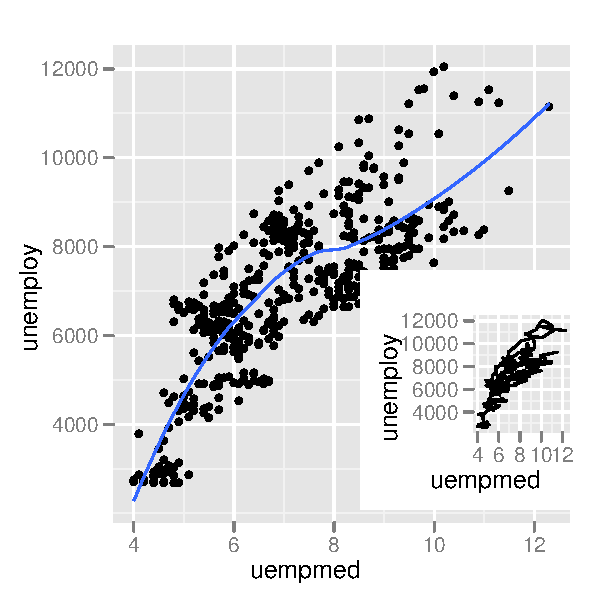
\includegraphics[width=0.5\textwidth]{polishing-subplot-1}
    \label{fig:subplot-1}
  }%
  \subfigure[Subplot tweaked for better display.]{
    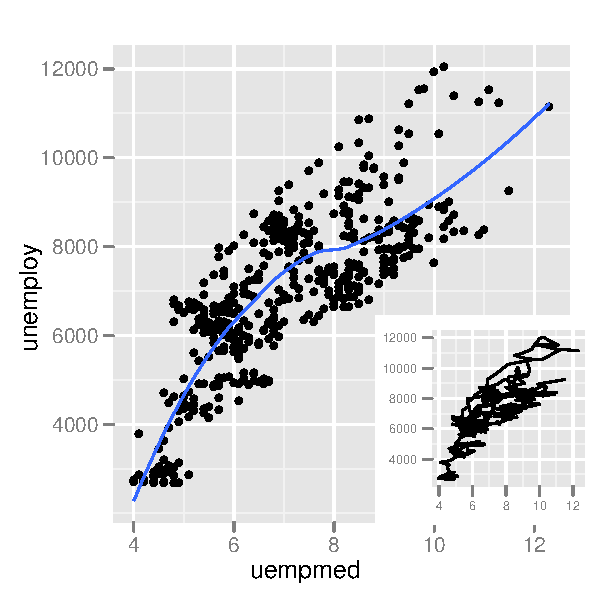
\includegraphics[width=0.5\textwidth]{polishing-subplot-2}
    \label{fig:subplot-2}
  }
  \caption{}
  \label{fig:subplot}
\end{figure}

By default, {\tt ggplot} always clears the screen and draws to the entire device.  You customise this in two ways. One way is to setup a viewport and push it on to the display, then draw the plot with {\tt newpage=FALSE}. {\tt pushViewport} adds the viewport to the list of viewports on the display.   Afterwards, {\tt upViewport} returns you to the viewport for the entire page, preparing you for the next set of output.

\subsection{Rectangular grids} 

A more complicated scenario is when you want to arrange a number of plots in a rectangular grid. Of course you could use the above technique to do so, but doing all the calculations by hand is cumbersome. The \f{grid.layout} function is a useful alternative, as it allows you to set up a regular grid of viewports with arbitrary heights and widths. You still need to create each viewport, but instead of explicitly specifying the position and size, you can specify the row and column of the layout.

% LISTING
% 
% vplayout <- function(x, y) 
%   viewport(layout.pos.row = x, layout.pos.col = y)
% grid.newpage()
% pushViewport(viewport(layout = grid.layout(2, 2)))
% 
% print(a, vp = vplayout(1, 1:2))
% print(b, vp = vplayout(2, 1))
% print(c, vp = vplayout(2, 2))
\input{_include/39720db87472ad6369ea76cd35ccac1b.tex}
% END

By default \f{grid.layout} creates makes each cell the same size, but you can use the \code{widths} and \code{heights} arguments to make them different sizes.

Note that since \f{ggsave} saves a single \ggplot plot to disk, it will not work with more complicated layouts.

\ifwhole
\else
  \bibliography{/Users/hadley/documents/phd/references}
  \end{document}
\fi

\chapter{Manipulating data}\label{cha:data}

So far this book has assumed you have your data in a nicely structured
data frame ready to feed to \texttt{ggplot()} or \texttt{qplot()}. If
this is not the case, then you'll need to do some transformation.

In \hyperref[sec:plyr]{an introduction to plyr}, you will learn how to
use the \textbf{plyr} package to reproduce the statistical
transformations performed by the layers, and then in
\hyperref[sec:melting]{converting data from wide to long} you will learn
a little about `molten' (or long) data, which is useful for time series
and parallel coordinates plots, among others.
\hyperref[sec:methods]{\texttt{ggplot()} methods} shows you how to write
methods that let you plot objects other than data frames, and
demonstrates how \texttt{ggplot} can be used to re-create a more
flexible version of the built in linear-model diagnostics.

Data cleaning, manipulation and transformation is a big topic and this
chapter only scratches the surface of topics closely related to
\texttt{ggplot}. I recommend the following references which go into
considerably more depth on this topic:

\begin{itemize}
\itemsep1pt\parskip0pt\parsep0pt
\item
  \emph{Data Manipulation with R}, by Phil Spector. Published by
  Springer, 2008.
\item
  ``plyr: divide and conquer for data analysis'', Hadley Wickham.
  Available from \url{http://had.co.nz/plyr}. This is a full description
  of the package used in \hyperref[sec:plyr]{an introduction to plyr}.
\item
  ``Reshaping data with the reshape package'', Hadley Wickham.
  \emph{Journal of Statistical Software}, 21(12), 2007.
  \url{http://www.jstatsoft.org/v21/i12/}. This describes the complement
  of the melt function used in \hyperref[sec:melting]{converting data
  from wide to long}, which can be used like pivot tables to create a
  wide range of data summaries and rearrangements.
\end{itemize}

\hyperdef{}{sec:plyr}{\section{An introduction to plyr}\label{sec:plyr}}

With faceting, \texttt{ggplot} makes it very easy to create identical
plots for different subsets of your data. \index{Package!plyr} This
section introduces \texttt{ddply()} from the \textbf{plyr} package, a
function that makes it easy to do the same thing for numerical
summaries. \textbf{plyr} provides a comprehensive suite of tools for
breaking up complicated data structures into pieces, processing each
piece and then joining the results back together. The \textbf{plyr}
package as a whole provides tools for breaking and combining lists,
arrays and data frames. Here we will focus on the \texttt{ddply()}
function which breaks up a data frame into subsets based on row values,
applies a function to each subset and then joins the results back into a
data frame. The basic syntax is
\texttt{ddply(.data, .variables, .fun, ...)}, where \indexf{ddply}

\begin{itemize}
\itemsep1pt\parskip0pt\parsep0pt
\item
  \texttt{.data} is the dataset to break up (e.g., the data that you are
  plotting).
\item
  \texttt{.variables} is a description of the grouping variables used to
  break up the dataset. This is written like \texttt{.(var1, var2)}, and
  to match the plot should contain all the grouping and faceting
  variables that you've used in the plot.
\item
  \texttt{.fun} is the summary function you want to use. The function
  can return a vector or data frame. The result does not need to contain
  the grouping variables: these will be added on automatically if
  they're needed. The result can be a much reduced aggregated dataset
  (maybe even one number), or the original data modified or expanded in
  some way.
\end{itemize}

More information and examples are available in the documentation,
\texttt{?ddply}, and on the package website,
\url{http://had.co.nz/plyr}. The following examples show a few useful
summary functions that solve common data manipulation problems.

\begin{itemize}
\itemsep1pt\parskip0pt\parsep0pt
\item
  Using \texttt{subset()} allows you to select the top (or bottom) n (or
  x\%) of observations in each group, or observations above (or below)
  some group-specific threshold: \indexf{subset}
\end{itemize}

\begin{Shaded}
\begin{Highlighting}[]
\CommentTok{# Select the smallest diamond in each colour}
\KeywordTok{ddply}\NormalTok{(diamonds, .(color), subset, carat ==}\StringTok{ }\KeywordTok{min}\NormalTok{(carat))}

\CommentTok{# Select the two smallest diamonds}
\KeywordTok{ddply}\NormalTok{(diamonds, .(color), subset, }\KeywordTok{order}\NormalTok{(carat) <=}\StringTok{ }\DecValTok{2}\NormalTok{)}

\CommentTok{# Select the 1% largest diamonds in each group}
\KeywordTok{ddply}\NormalTok{(diamonds, .(color), subset, carat >}\StringTok{ }
\StringTok{        }\KeywordTok{quantile}\NormalTok{(carat, }\FloatTok{0.99}\NormalTok{))}

\CommentTok{# Select all diamonds bigger than the group average}
\KeywordTok{ddply}\NormalTok{(diamonds, .(color), subset, price >}\StringTok{ }\KeywordTok{mean}\NormalTok{(price))}
\end{Highlighting}
\end{Shaded}

\begin{itemize}
\itemsep1pt\parskip0pt\parsep0pt
\item
  Using \texttt{transform()} allows you to perform group-wise
  transformations with very little work. This is particularly useful if
  you want to add new variables that are calculated on a per-group
  level, such as a per-group standardisation.
  \hyperref[sub:time-series]{Multiple time series} shows another use of
  this technique for standardising time series to a common scale.
  \index{Transformation!group-wise} \indexf{transform}
\end{itemize}

\begin{Shaded}
\begin{Highlighting}[]
\CommentTok{# Within each colour, scale price to mean 0 and variance 1}
\KeywordTok{ddply}\NormalTok{(diamonds, .(color), transform, }\DataTypeTok{price =} \KeywordTok{scale}\NormalTok{(price))}

\CommentTok{# Subtract off group mean}
\KeywordTok{ddply}\NormalTok{(diamonds, .(color), transform, }
      \DataTypeTok{price =} \NormalTok{price -}\StringTok{ }\KeywordTok{mean}\NormalTok{(price))}
\end{Highlighting}
\end{Shaded}

\begin{itemize}
\itemsep1pt\parskip0pt\parsep0pt
\item
  If you want to apply a function to every column in the data frame, you
  might find the \texttt{colwise()} function handy. This function
  converts a function that operates on vectors to a function that
  operates column-wise on data frames. This is rather different than
  most functions: instead of returning a vector of numbers,
  \texttt{colwise()} returns a new function. The following example
  creates a function to count the number of missing values in a vector
  and then shows how we can use \texttt{colwise()} to apply it to every
  column in a data frame. \index{Transformation!column-wise}
  \indexf{colwise}
\end{itemize}

\begin{Shaded}
\begin{Highlighting}[]
\NormalTok{nmissing <-}\StringTok{ }\NormalTok{function(x) }\KeywordTok{sum}\NormalTok{(}\KeywordTok{is.na}\NormalTok{(x))}
\KeywordTok{nmissing}\NormalTok{(msleep$name)}
\CommentTok{#> [1] 0}
\KeywordTok{nmissing}\NormalTok{(msleep$brainwt)}
\CommentTok{#> [1] 27}

\NormalTok{nmissing_df <-}\StringTok{ }\KeywordTok{colwise}\NormalTok{(nmissing)}
\KeywordTok{nmissing_df}\NormalTok{(msleep)}
\CommentTok{#>   name genus vore order conservation sleep_total sleep_rem}
\CommentTok{#> 1    0     0    7     0           29           0        22}
\CommentTok{#>   sleep_cycle awake brainwt bodywt}
\CommentTok{#> 1          51     0      27      0}
\CommentTok{# This is shorthand for the previous two steps}
\KeywordTok{colwise}\NormalTok{(nmissing)(msleep)}
\CommentTok{#>   name genus vore order conservation sleep_total sleep_rem}
\CommentTok{#> 1    0     0    7     0           29           0        22}
\CommentTok{#>   sleep_cycle awake brainwt bodywt}
\CommentTok{#> 1          51     0      27      0}
\end{Highlighting}
\end{Shaded}

The specialised version \texttt{numcolwise()} does the same thing, but
works only with numeric columns. For example,
\texttt{numcolwise(median)} will calculate a median for every numeric
column, or \texttt{numcolwise(quantile)} will calculate quantiles for
every numeric column. Similarly, \texttt{catcolwise()} only works with
categorical columns. \indexf{numcolwise} \indexf{catcolwise}

\begin{Shaded}
\begin{Highlighting}[]
\NormalTok{msleep2 <-}\StringTok{ }\NormalTok{msleep[, -}\DecValTok{6}\NormalTok{] }\CommentTok{# Remove a column to save space}
\KeywordTok{numcolwise}\NormalTok{(median)(msleep2, }\DataTypeTok{na.rm =} \NormalTok{T)}
\CommentTok{#>   sleep_rem sleep_cycle awake brainwt bodywt}
\CommentTok{#> 1       1.5        0.33    14   0.012    1.7}
\KeywordTok{numcolwise}\NormalTok{(quantile)(msleep2, }\DataTypeTok{na.rm =} \NormalTok{T)}
\CommentTok{#>   sleep_rem sleep_cycle awake brainwt  bodywt}
\CommentTok{#> 1       0.1        0.12   4.1 0.00014 5.0e-03}
\CommentTok{#> 2       0.9        0.18  10.2 0.00290 1.7e-01}
\CommentTok{#> 3       1.5        0.33  13.9 0.01240 1.7e+00}
\CommentTok{#> 4       2.4        0.58  16.1 0.12550 4.2e+01}
\CommentTok{#> 5       6.6        1.50  22.1 5.71200 6.7e+03}
\KeywordTok{numcolwise}\NormalTok{(quantile)(msleep2, }\DataTypeTok{probs =} \KeywordTok{c}\NormalTok{(}\FloatTok{0.25}\NormalTok{, }\FloatTok{0.75}\NormalTok{), }
                     \DataTypeTok{na.rm =} \NormalTok{T)}
\CommentTok{#>   sleep_rem sleep_cycle awake brainwt bodywt}
\CommentTok{#> 1       0.9        0.18    10  0.0029   0.17}
\CommentTok{#> 2       2.4        0.58    16  0.1255  41.75}
\end{Highlighting}
\end{Shaded}

Combined with \texttt{ddply()}, this makes it easy to produce per-group
summaries: \index{Summary!group-wise}

\begin{Shaded}
\begin{Highlighting}[]
\KeywordTok{ddply}\NormalTok{(msleep2, .(vore), }\KeywordTok{numcolwise}\NormalTok{(median), }\DataTypeTok{na.rm =} \NormalTok{T)}
\CommentTok{#>      vore sleep_rem sleep_cycle awake brainwt bodywt}
\CommentTok{#> 1   carni      1.95        0.38  13.6  0.0445 20.490}
\CommentTok{#> 2   herbi      0.95        0.22  13.7  0.0123  1.225}
\CommentTok{#> 3 insecti      3.00        0.17   5.9  0.0012  0.075}
\CommentTok{#> 4    omni      1.85        0.50  14.1  0.0066  0.950}
\CommentTok{#> 5    <NA>      2.00        0.18  13.4  0.0030  0.122}
\KeywordTok{ddply}\NormalTok{(msleep2, .(vore), }\KeywordTok{numcolwise}\NormalTok{(mean), }\DataTypeTok{na.rm =} \NormalTok{T)}
\CommentTok{#>      vore sleep_rem sleep_cycle awake brainwt bodywt}
\CommentTok{#> 1   carni       2.3        0.37  13.6  0.0793  90.75}
\CommentTok{#> 2   herbi       1.4        0.42  14.5  0.6216 366.88}
\CommentTok{#> 3 insecti       3.5        0.16   9.1  0.0215  12.92}
\CommentTok{#> 4    omni       2.0        0.59  13.1  0.1457  12.72}
\CommentTok{#> 5    <NA>       1.9        0.18  13.8  0.0076   0.86}
\end{Highlighting}
\end{Shaded}

\begin{itemize}
\itemsep1pt\parskip0pt\parsep0pt
\item
  If none of the previous shortcuts is appropriate, make your own
  summary function which takes a data frame as input and returns an
  appropriately summarised data frame as output. The following function
  calculates the rank correlation of price and carat and compares it to
  the regular correlation of the logged values.
\end{itemize}

\begin{Shaded}
\begin{Highlighting}[]
\NormalTok{my_summary <-}\StringTok{ }\NormalTok{function(df) \{}
  \KeywordTok{with}\NormalTok{(df, }\KeywordTok{data.frame}\NormalTok{(}
    \DataTypeTok{pc_cor =} \KeywordTok{cor}\NormalTok{(price, carat, }\DataTypeTok{method =} \StringTok{"spearman"}\NormalTok{),}
    \DataTypeTok{lpc_cor =} \KeywordTok{cor}\NormalTok{(}\KeywordTok{log}\NormalTok{(price), }\KeywordTok{log}\NormalTok{(carat))}
    \NormalTok{))}
\NormalTok{\}}
\KeywordTok{ddply}\NormalTok{(diamonds, .(cut), my_summary)}
\CommentTok{#>         cut pc_cor lpc_cor}
\CommentTok{#> 1      Fair   0.91    0.91}
\CommentTok{#> 2      Good   0.96    0.97}
\CommentTok{#> 3 Very Good   0.97    0.97}
\CommentTok{#> 4   Premium   0.96    0.97}
\CommentTok{#> 5     Ideal   0.95    0.97}
\KeywordTok{ddply}\NormalTok{(diamonds, .(color), my_summary)}
\CommentTok{#>   color pc_cor lpc_cor}
\CommentTok{#> 1     D   0.96    0.96}
\CommentTok{#> 2     E   0.96    0.96}
\CommentTok{#> 3     F   0.96    0.96}
\CommentTok{#> 4     G   0.96    0.97}
\CommentTok{#> 5     H   0.97    0.98}
\CommentTok{#> 6     I   0.98    0.99}
\CommentTok{#> 7     J   0.98    0.99}
\end{Highlighting}
\end{Shaded}

Note how our summary function did not need to output the group
variables. This makes it much easier to aggregate over different groups.

The common pattern of all these problems is that they are easy to solve
if we have the right subset. Often the solution for a single case might
be a single line of code. The difficulty comes when we want to apply the
function to multiple subsets and then correctly join back up the
results. This may take a lot of code, especially if you want to preserve
group labels. \texttt{ddply()} takes care of all this for you.

The following case study shows how you can use \textbf{plyr} to
reproduce the statistical summaries produced by \texttt{ggplot}. This is
useful if you want to save them to disk or apply them to other datasets.
It's also useful to be able to check that \texttt{ggplot} is doing
exactly what you think!

\subsection{Fitting multiple models}\label{sub:multiple-models}

In this section, we'll work through the process of generating the
smoothed data produced by \texttt{stat\_smooth()}. This process will be
the same for any other statistic, and should allow you to produce more
complex summaries that \texttt{ggplot} can't produce by itself.
Figure\textasciitilde{}\ref{fig:smooth} shows the group-wise smoothes
produced by the following code. \index{Model!fitting multiple models}
\indexf{stat_smooth}

\begin{Shaded}
\begin{Highlighting}[]
\KeywordTok{qplot}\NormalTok{(carat, price, }\DataTypeTok{data =} \NormalTok{diamonds, }\DataTypeTok{geom =} \StringTok{"smooth"}\NormalTok{, }
  \DataTypeTok{colour =} \NormalTok{color)}
\NormalTok{dense <-}\StringTok{ }\KeywordTok{subset}\NormalTok{(diamonds, carat <}\StringTok{ }\DecValTok{2}\NormalTok{)}
\KeywordTok{qplot}\NormalTok{(carat, price, }\DataTypeTok{data =} \NormalTok{dense, }\DataTypeTok{geom =} \StringTok{"smooth"}\NormalTok{, }
  \DataTypeTok{colour =} \NormalTok{color,  }\DataTypeTok{fullrange =} \OtherTok{TRUE}\NormalTok{)}
\end{Highlighting}
\end{Shaded}

\begin{figure}
\includegraphics[width=0.49\linewidth]{figures/datasmooth-1} \includegraphics[width=0.49\linewidth]{figures/datasmooth-2} \caption{A plot showing the smoothed trends for price vs. carat for each colour of diamonds. With the full range of carats (left), the standard errors balloon after around two carats because there are relatively few diamonds of that size. Restricting attention to diamonds of less than two carats (right) focuses on the region where we have plenty of data.\label{fig:smooth}}
\end{figure}

How can we re-create this by hand? First we read the
\texttt{stat\_smooth()} documentation to determine what the model is:
for large data it's \texttt{gam(y \textasciitilde{} s(x, bs = "cs"))}.
To get the same output as \texttt{stat\_smooth()}, we need to fit the
model, then predict it on an evenly spaced grid of points. This task is
performed by the \texttt{smooth()} function in the following code. Once
we have written this function it is straightforward to apply it to each
diamond colour using \texttt{ddply()}. \index{Package!mgcv}

Figure\textasciitilde{}\ref{fig:smooth-by-hand} shows the results of
this work, which are identical to what we got with \texttt{ggplot} doing
all the work.

\begin{Shaded}
\begin{Highlighting}[]
\KeywordTok{library}\NormalTok{(mgcv)}
\NormalTok{smooth <-}\StringTok{ }\NormalTok{function(df) \{}
  \NormalTok{mod <-}\StringTok{ }\KeywordTok{gam}\NormalTok{(price ~}\StringTok{ }\KeywordTok{s}\NormalTok{(carat, }\DataTypeTok{bs =} \StringTok{"cs"}\NormalTok{), }\DataTypeTok{data =} \NormalTok{df)}
  \NormalTok{grid <-}\StringTok{ }\KeywordTok{data.frame}\NormalTok{(}\DataTypeTok{carat =} \KeywordTok{seq}\NormalTok{(}\FloatTok{0.2}\NormalTok{, }\DecValTok{2}\NormalTok{, }\DataTypeTok{length =} \DecValTok{50}\NormalTok{))}
  \NormalTok{pred <-}\StringTok{ }\KeywordTok{predict}\NormalTok{(mod, grid, }\DataTypeTok{se =} \NormalTok{T)}
  
  \NormalTok{grid$price <-}\StringTok{ }\NormalTok{pred$fit}
  \NormalTok{grid$se <-}\StringTok{ }\NormalTok{pred$se.fit}
  \NormalTok{grid}
\NormalTok{\}}
\NormalTok{smoothes <-}\StringTok{ }\KeywordTok{ddply}\NormalTok{(dense, .(color), smooth)}
\KeywordTok{qplot}\NormalTok{(carat, price, }\DataTypeTok{data =} \NormalTok{smoothes, }\DataTypeTok{colour =} \NormalTok{color, }
  \DataTypeTok{geom =} \StringTok{"line"}\NormalTok{)}
\KeywordTok{qplot}\NormalTok{(carat, price, }\DataTypeTok{data =} \NormalTok{smoothes, }\DataTypeTok{colour =} \NormalTok{color, }
  \DataTypeTok{geom =} \StringTok{"smooth"}\NormalTok{, }\DataTypeTok{ymax =} \NormalTok{price +}\StringTok{ }\DecValTok{2} \NormalTok{*}\StringTok{ }\NormalTok{se, }\DataTypeTok{ymin =} \NormalTok{price -}\StringTok{ }\DecValTok{2} \NormalTok{*}\StringTok{ }\NormalTok{se)}
\end{Highlighting}
\end{Shaded}

\begin{figure}
\includegraphics[width=0.49\linewidth]{figures/datasmooth-by-hand-1} \includegraphics[width=0.49\linewidth]{figures/datasmooth-by-hand-2} \caption{Figure~\ref{fig:smooth} with all statistical calculations performed by hand.  The predicted values (left), and with standard errors (right).\label{fig:smooth-by-hand}}
\end{figure}

Doing the summary by hand gives you much more flexibility to fit models
where the grouping factor is explicitly included as a covariate. For
example, the following model models price as a non-linear function of
carat, plus a constant term for each colour. It's not a very good model
as it predicts negative prices for small, poor-quality diamonds, but
it's a starting point for a better model.

\begin{Shaded}
\begin{Highlighting}[]
\NormalTok{>}\StringTok{ }\NormalTok{mod <-}\StringTok{ }\KeywordTok{gam}\NormalTok{(price ~}\StringTok{ }\KeywordTok{s}\NormalTok{(carat, }\DataTypeTok{bs =} \StringTok{"cs"}\NormalTok{) +}\StringTok{ }\NormalTok{color, }\DataTypeTok{data =} \NormalTok{dense)}
\NormalTok{>}\StringTok{ }\NormalTok{grid <-}\StringTok{ }\KeywordTok{with}\NormalTok{(diamonds, }\KeywordTok{expand.grid}\NormalTok{(}
\NormalTok{+}\StringTok{   }\DataTypeTok{carat =} \KeywordTok{seq}\NormalTok{(}\FloatTok{0.2}\NormalTok{, }\DecValTok{2}\NormalTok{, }\DataTypeTok{length =} \DecValTok{50}\NormalTok{),}
\NormalTok{+}\StringTok{   }\DataTypeTok{color =} \KeywordTok{levels}\NormalTok{(color)}
\NormalTok{+}\StringTok{ }\NormalTok{))}
\NormalTok{>}\StringTok{ }\NormalTok{grid$pred <-}\StringTok{ }\KeywordTok{predict}\NormalTok{(mod, grid)}
\NormalTok{>}\StringTok{ }\KeywordTok{qplot}\NormalTok{(carat, pred, }\DataTypeTok{data =} \NormalTok{grid, }\DataTypeTok{colour =} \NormalTok{color, }\DataTypeTok{geom =} \StringTok{"line"}\NormalTok{)}
\end{Highlighting}
\end{Shaded}

\includegraphics[width=0.49\linewidth]{figures/datagam-1}

See also \hyperref[sub:different-aesthetics]{varying aesthetics and
data} and \hyperref[sec:uncertainty]{revealing uncertainty} for other
ways of combining models and data.

\hyperdef{}{sec:melting}{\section{Converting data from wide to
long}\label{sec:melting}}

In \texttt{ggplot} graphics, groups are defined by rows, not by columns.
This makes it easy to draw a line for each group defined by the value of
a variable (or set of variables) but difficult to draw a separate line
for each variable. In this section you will learn how to transform your
data to a form in which you can draw a line for each variable. This
transformation converts from `wide' data to `long' data, where each
variable now occupies its own set of rows. \index{Data!wide-to-long}
\index{Converting data!from wide to long}

To perform this transformation we will use the \texttt{melt()} function
from the \textbf{reshape} package (Wickham 2007). Reshape also provides
the \texttt{cast()} function to flexibly reshape and aggregate data,
which you may want to read about yourself.
Table\textasciitilde{}\ref{tbl:melt} gives an example. The
\texttt{melt()} function has three arguments: \index{Package!reshape}
\indexf{melt}

\begin{itemize}
\itemsep1pt\parskip0pt\parsep0pt
\item
  \texttt{data}: the data frame you want to convert to long form.
\item
  \texttt{id.vars}: Identifier (id) variables identify the unit that
  measurements take place on. Id variables are usually discrete, and are
  typically fixed by design. In \texttt{anova()} notation (\(Y_{ijk}\)),
  id variables are the indices on the variables (\(i, j, k\)); in
  database notation, id variables are a composite primary key.
\item
  \texttt{measure.vars}: Measured variables represent what is measured
  on that unit (\(Y\)). These will be the variables that you want to
  display simultaneously on the plot.
\end{itemize}

If you're familiar with Wilkinson's grammar of graphics, you might
wonder why there is no equivalent to the algebra. There is no equivalent
to the algebra within \texttt{ggplot} itself because there are many
other facilities for transforming data in R, and it is in line with the
\texttt{ggplot} philosophy of keeping data transformation and
visualisation as separate as possible.

\begin{table}[ht]
\centering
\begin{tabular}{rlr}
  \hline
date & variable & value \\ 
  \hline
-916.00 & pce & 507.80 \\ 
  -885.00 & pce & 510.90 \\ 
  -854.00 & pce & 516.70 \\ 
  -824.00 & pce & 513.30 \\ 
  -793.00 & pce & 518.50 \\ 
  -763.00 & pce & 526.20 \\ 
   \hline
\end{tabular}
\caption{Economics data in wide, left, and long, right, formats. The data stored in each table is equivalent, just the arrangement is different. It it easy to use the wider format with \texttt{ggplot} to produce a line for each variable.} 
\label{melt}
\end{table}

The following sections explore two important uses of molten data in more
detail: plotting multiple time series and creating parallel coordinate
plots. You will also see how to use \texttt{ddply()} to rescale the
variables, and learn about the features of \texttt{ggplot} that are most
useful in conjunction with this sort of data.

\hyperdef{}{sub:time-series}{\subsection{Multiple time
series}\label{sub:time-series}}

Take the \texttt{economics} dataset. It contains information about
monthly economic data like the number of people unemployed
(\texttt{unemploy}) and the median length of unemployment
(\texttt{uempmed}). We might expect these two variables to be related.
Each of these variables is stored in a column, which makes it easy to
compare them with a scatterplot, and draw individual time series, as
shown in Figure\textasciitilde{}\ref{fig:series-wide}. But what if we
want to see the time series simultaneously?
\index{Time series!multivariate} \indexf{geom_line}

\begin{Shaded}
\begin{Highlighting}[]
\KeywordTok{qplot}\NormalTok{(date, uempmed, }\DataTypeTok{data =} \NormalTok{economics, }\DataTypeTok{geom =} \StringTok{"line"}\NormalTok{)}
\KeywordTok{qplot}\NormalTok{(date, unemploy, }\DataTypeTok{data =} \NormalTok{economics, }\DataTypeTok{geom =} \StringTok{"line"}\NormalTok{)}
\KeywordTok{qplot}\NormalTok{(unemploy, uempmed, }\DataTypeTok{data =} \NormalTok{economics) +}\StringTok{ }\KeywordTok{geom_smooth}\NormalTok{()}
\end{Highlighting}
\end{Shaded}

\begin{figure}
\includegraphics[width=0.32\linewidth]{figures/dataseries-wide-1} \includegraphics[width=0.32\linewidth]{figures/dataseries-wide-2} \includegraphics[width=0.32\linewidth]{figures/dataseries-wide-3} \caption{When the economics dataset is stored in wide format, it is easy to create separate time series plots for each variable (left and centre), and easy to create scatterplots comparing them (right).\label{fig:series-wide}}
\end{figure}

One way is to build up the plot with a different layer for each
variable, as you saw in \hyperref[sub:scale-manual]{the manual discrete
scale}. However, this quickly becomes tedious when you have many
variables, and a better alternative is to melt the data into a long
format and then visualise that. In the molten data the time series have
their value stored in the \texttt{value} variable and we can distinguish
between them with the \texttt{variable} variable. The code below shows
these two alternatives. The plots they produce are very similar, and are
shown in Figure\textasciitilde{}\ref{fig:series-methods}.

\begin{Shaded}
\begin{Highlighting}[]
\KeywordTok{ggplot}\NormalTok{(economics, }\KeywordTok{aes}\NormalTok{(date)) +}\StringTok{ }
\StringTok{  }\KeywordTok{geom_line}\NormalTok{(}\KeywordTok{aes}\NormalTok{(}\DataTypeTok{y =} \NormalTok{unemploy, }\DataTypeTok{colour =} \StringTok{"unemploy"}\NormalTok{)) +}\StringTok{ }
\StringTok{  }\KeywordTok{geom_line}\NormalTok{(}\KeywordTok{aes}\NormalTok{(}\DataTypeTok{y =} \NormalTok{uempmed, }\DataTypeTok{colour =} \StringTok{"uempmed"}\NormalTok{)) +}\StringTok{ }
\StringTok{  }\KeywordTok{scale_colour_hue}\NormalTok{(}\StringTok{"variable"}\NormalTok{)}

\NormalTok{emp <-}\StringTok{ }\NormalTok{tidyr::}\KeywordTok{gather}\NormalTok{(economics, variable, value, uempmed, unemploy)}
\KeywordTok{qplot}\NormalTok{(date, value, }\DataTypeTok{data =} \NormalTok{emp, }\DataTypeTok{geom =} \StringTok{"line"}\NormalTok{, }\DataTypeTok{colour =} \NormalTok{variable)}
\end{Highlighting}
\end{Shaded}

\begin{figure}
\includegraphics[width=0.49\linewidth]{figures/dataseries-methods-1} \includegraphics[width=0.49\linewidth]{figures/dataseries-methods-2} \caption{The two methods of displaying both series on a single plot produce identical plots, but using long data is much easier when you have many variables.  The series have radically different scales, so we only see the pattern in the \texttt{unemploy} variable. You might not even notice \texttt{uempmed} unless you're paying close attention: it's the line at the bottom of the plot.\label{fig:series-methods}}
\end{figure}

There is a problem with these plots: the two variables have radically
different scales, and so the series for \texttt{uempmed} appears as a
flat line at the bottom of the plot. There is no way to produce a plot
with two axes in \texttt{ggplot} because this type of plot is
fundamentally misleading. Instead there are two perceptually
well-founded alternatives: rescale the variables to have a common range,
or use faceting with free scales. These alternatives are created with
the code below and are shown in
Figure\textasciitilde{}\ref{fig:series-scaling}. \index{Axis!multiple}

\begin{Shaded}
\begin{Highlighting}[]
\NormalTok{range01 <-}\StringTok{ }\NormalTok{function(x) \{}
  \NormalTok{rng <-}\StringTok{ }\KeywordTok{range}\NormalTok{(x, }\DataTypeTok{na.rm =} \OtherTok{TRUE}\NormalTok{)}
  \NormalTok{(x -}\StringTok{ }\NormalTok{rng[}\DecValTok{1}\NormalTok{]) /}\StringTok{ }\KeywordTok{diff}\NormalTok{(rng)}
\NormalTok{\}}
\NormalTok{emp2 <-}\StringTok{ }\KeywordTok{ddply}\NormalTok{(emp, .(variable), transform, }\DataTypeTok{value =} \KeywordTok{range01}\NormalTok{(value))}
\KeywordTok{qplot}\NormalTok{(date, value, }\DataTypeTok{data =} \NormalTok{emp2, }\DataTypeTok{geom =} \StringTok{"line"}\NormalTok{, }
  \DataTypeTok{colour =} \NormalTok{variable, }\DataTypeTok{linetype =} \NormalTok{variable)}
\KeywordTok{qplot}\NormalTok{(date, value, }\DataTypeTok{data =} \NormalTok{emp, }\DataTypeTok{geom =} \StringTok{"line"}\NormalTok{) +}\StringTok{ }
\StringTok{  }\KeywordTok{facet_grid}\NormalTok{(variable ~}\StringTok{ }\NormalTok{., }\DataTypeTok{scales =} \StringTok{"free_y"}\NormalTok{)}
\end{Highlighting}
\end{Shaded}

\begin{figure}
\includegraphics[width=0.49\linewidth]{figures/dataseries-scaling-1} \includegraphics[width=0.49\linewidth]{figures/dataseries-scaling-2} \caption{When the series have very different scales we have two alternatives: left, rescale the variables to a common scale, or right, display the variables on separate facets and using free scales.\label{fig:series-scaling}}
\end{figure}

\subsection{Parallel coordinates plot}\label{sub:molten-data}

In a similar manner, we can use molten data to create a parallel
coordinates plot (Inselberg 1985,wegman:1990), which has the `variable'
variable on the x axis and value on the y axis. We need a new variable
to record the row that each observation came from, which is used as a
grouping variable for the lines (so we get one line per observation).
The easiest value to use for this is the data frame \texttt{rownames},
and we give it an unusual name \texttt{.row}, so we don't squash any of
the existing variables. Once we have the data in this form, creating a
parallel coordinates plot is easy. \index{Parallel coordinates plot}

The following code does exactly that for the ratings of 840 movies with
over 10,000 votes. This dataset has a moderate number of variables (10)
and many cases, and will allow us to experiment with a common technique
for dealing with large data in parallel coordinates plots: transparency
and clustering. Each variable gives the proportion of votes given to
each rating between 0 (very bad) and 10 (very good). Since this data is
already on a common scale we don't need to rescale it, but in general,
we would need to use the technique from the previous section to ensure
the variables are comparable. This is particularly important if we are
going to use other multidimensional techniques to analyse the data.
\index{Rescaling}

\begin{Shaded}
\begin{Highlighting}[]
\NormalTok{popular <-}\StringTok{ }\KeywordTok{subset}\NormalTok{(movies, votes >}\StringTok{ }\FloatTok{1e4}\NormalTok{)}
\NormalTok{ratings <-}\StringTok{ }\NormalTok{popular[, }\DecValTok{7}\NormalTok{:}\DecValTok{16}\NormalTok{]}
\NormalTok{ratings$.row <-}\StringTok{ }\KeywordTok{rownames}\NormalTok{(ratings)}
\NormalTok{molten <-}\StringTok{ }\NormalTok{tidyr::}\KeywordTok{gather}\NormalTok{(ratings, variable, value, -.row)}
\end{Highlighting}
\end{Shaded}

Once the data is in this form, creating a parallel coordinates plot is
easy. All we need is a line plot with \texttt{variable} on the x axis,
\texttt{value} on the y axis and the lines grouped by \texttt{.row}.
This data needs a few tweaks to the default because the values are
highly discrete. In the following code, we experiment with jittering and
alpha blending to better display where the bulk of the movies lie. The
results are shown in Figure\textasciitilde{}\ref{fig:pcp}. Most are
rated as sevens or eights by around 25\% of voters, with a few
exceptional movies getting 35\% of more perfect 10s. However, the large
number of lines makes it difficult to distinguish individual movies and
it's hard to draw firm conclusions. \indexf{geom_line}

\begin{Shaded}
\begin{Highlighting}[]
\NormalTok{pcp <-}\StringTok{ }\KeywordTok{ggplot}\NormalTok{(molten, }\KeywordTok{aes}\NormalTok{(variable, value, }\DataTypeTok{group =} \NormalTok{.row))}
\NormalTok{pcp +}\StringTok{ }\KeywordTok{geom_line}\NormalTok{()}
\NormalTok{pcp +}\StringTok{ }\KeywordTok{geom_line}\NormalTok{(}\DataTypeTok{alpha =} \DecValTok{1} \NormalTok{/}\StringTok{ }\DecValTok{20}\NormalTok{)}
\NormalTok{jit <-}\StringTok{ }\KeywordTok{position_jitter}\NormalTok{(}\DataTypeTok{width =} \FloatTok{0.25}\NormalTok{, }\DataTypeTok{height =} \FloatTok{2.5}\NormalTok{)}
\NormalTok{pcp +}\StringTok{ }\KeywordTok{geom_line}\NormalTok{(}\DataTypeTok{position =} \NormalTok{jit)}
\NormalTok{pcp +}\StringTok{ }\KeywordTok{geom_line}\NormalTok{(}\DataTypeTok{alpha =} \DecValTok{1} \NormalTok{/}\StringTok{ }\DecValTok{20}\NormalTok{, }\DataTypeTok{position =} \NormalTok{jit)}
\end{Highlighting}
\end{Shaded}

\begin{figure}
\includegraphics[width=0.49\linewidth]{figures/datapcp-1} \includegraphics[width=0.49\linewidth]{figures/datapcp-2} \includegraphics[width=0.49\linewidth]{figures/datapcp-3} \includegraphics[width=0.49\linewidth]{figures/datapcp-4} \caption{Variants on the parallel coordinates plot to better display the patterns in this highly discrete data.  To improve the default pcp (top left) we experiment with alpha blending (top right), jittering (bottom left) and then both together (bottom right).\label{fig:pcp}}
\end{figure}

To make the patterns more clear we will cluster the movies into groups
of similar rating patterns. The following code uses kmeans clustering
(Hartigan and Wong 1979) to produce six groups of similar movies. To
make the clusters a little more interpretable, they are relabelled so
that cluster 1 has the lowest average rating and cluster six the
highest. \index{Clustering}

\begin{Shaded}
\begin{Highlighting}[]
\NormalTok{cl <-}\StringTok{ }\KeywordTok{kmeans}\NormalTok{(ratings[}\DecValTok{1}\NormalTok{:}\DecValTok{10}\NormalTok{], }\DecValTok{6}\NormalTok{)}
\NormalTok{ratings$cluster <-}\StringTok{ }\KeywordTok{reorder}\NormalTok{(}\KeywordTok{factor}\NormalTok{(cl$cluster), popular$rating)}
\KeywordTok{levels}\NormalTok{(ratings$cluster) <-}\StringTok{ }\KeywordTok{seq_along}\NormalTok{(}\KeywordTok{levels}\NormalTok{(ratings$cluster))}
\NormalTok{molten <-}\StringTok{ }\NormalTok{tidyr::}\KeywordTok{gather}\NormalTok{(ratings, variable, value, r1:r10)}
\end{Highlighting}
\end{Shaded}

There are many different ways that we can visualise the result of this
clustering. One popular method is shown in
Figure\textasciitilde{}\ref{fig:pcp-colour} where line colour is mapped
to group membership. This plot is supplemented with a plot that just
shows averages for each group. These plots are both straightforward to
create, as shown in the following code.

\begin{Shaded}
\begin{Highlighting}[]
\NormalTok{pcp_cl <-}\StringTok{ }\KeywordTok{ggplot}\NormalTok{(molten, }
  \KeywordTok{aes}\NormalTok{(variable, value, }\DataTypeTok{group =} \NormalTok{.row, }\DataTypeTok{colour =} \NormalTok{cluster)) }
\NormalTok{pcp_cl +}\StringTok{ }\KeywordTok{geom_line}\NormalTok{(}\DataTypeTok{position =} \NormalTok{jit, }\DataTypeTok{alpha =} \DecValTok{1}\NormalTok{/}\DecValTok{5}\NormalTok{)}
\NormalTok{pcp_cl +}\StringTok{ }\KeywordTok{stat_summary}\NormalTok{(}\KeywordTok{aes}\NormalTok{(}\DataTypeTok{group =} \NormalTok{cluster), }\DataTypeTok{fun.y =} \NormalTok{mean, }
  \DataTypeTok{geom =} \StringTok{"line"}\NormalTok{)}
\end{Highlighting}
\end{Shaded}

\begin{figure}
\includegraphics[width=0.49\linewidth]{figures/datapcp-colour-1} \includegraphics[width=0.49\linewidth]{figures/datapcp-colour-2} \caption{Displaying cluster membership on a parallel coordinates plot. (Left) Individual movies coloured by group membership and (right) group means.\label{fig:pcp-colour}}
\end{figure}

These plots are good for showing the differences between groups, but
they don't tell us a lot about whether we've done a good job clustering
the data. Figure\textasciitilde{}\ref{fig:pcp-facet} uses faceting to
display each group in its own panel. This plot highlights the variation
within many of the groups, suggesting that perhaps more clusters would
be appropriate.

\begin{Shaded}
\begin{Highlighting}[]
\NormalTok{pcp_cl +}\StringTok{ }\KeywordTok{geom_line}\NormalTok{(}\DataTypeTok{position =} \NormalTok{jit, }\DataTypeTok{alpha =} \DecValTok{1}\NormalTok{/}\DecValTok{5}\NormalTok{) +}
\StringTok{  }\KeywordTok{facet_wrap}\NormalTok{(~}\StringTok{ }\NormalTok{cluster)}
\end{Highlighting}
\end{Shaded}

\begin{figure}
\includegraphics[width=\linewidth]{figures/datapcp-facet-1} \caption{Faceting allows us to display each group in its own panel, highlighting the fact that there seems to be considerable variation within each group, and suggesting that we need more groups in our clustering.\label{fig:pcp-facet}}
\end{figure}

\hyperdef{}{sec:methods}{\section{\texttt{ggplot()}
methods}\label{sec:methods}}

\texttt{ggplot()} is a generic function, with different methods for
different types of data. The most common input, and what we have used
until now, is a data frame. As with base and lattice graphics, it is
possible to extend \texttt{ggplot()} to work with other types of data.
However, the way this works with \texttt{ggplot} is fundamentally
different: \texttt{ggplot()} will not give you a complete plot, but
instead will give you the tools you need to make any plot you desire.
\index{ggplot!methods}

This process is mediated by the \texttt{fortify()} method, which takes
an object, and optional data frame, and creates a version of the object
in a form suitable for plotting with \texttt{ggplot}, i.e., as a data
frame. The name fortify comes from thinking about combining a model with
its data: the model fortifies the data, and the data fortifies the
model, and the result can be used to simultaneously visualise the model
and the data. An example will make this concrete, as you will see when
we describe the fortify method for linear models. \index{Fortify}
\indexf{fortify}

This section describes how the \texttt{fortify()} method works, and how
you can create new methods that are aligned with the \texttt{ggplot}
philosophy. The most important philosophical consideration is that data
transformation and display should be kept as separate as possible. This
maximises reusability, as you are no longer trapped into the single
display that the author envisaged.

These different types of input also work with \texttt{qplot()}: remember
that \texttt{qplot()} is just a thin wrapper around \texttt{ggplot()}.

\subsection{Linear models}

Currently, \texttt{ggplot} provides only one fortify method, for linear
models. Here we'll show how this method works, and how you can use it to
create tailored plots for better understanding your data and models.
Figure\textasciitilde{}\ref{fig:plot-lm} shows the output of
\texttt{plot.lm()} for a simple model. The graphics are a set of
pre-chosen model summary plots. These are useful for particular
problems, but are completely inflexible: there is no way to modify them
apart from opening up the source code for \texttt{plot.lm()} and
modifying it. This is hard because the data transformation and display
are inextricably entangled, making the code difficult to understand.
\index{Model!diagnostics} \index{Model!linear} \index{Linear models}
\indexf{fortify.lm}

\begin{Shaded}
\begin{Highlighting}[]
\NormalTok{mod <-}\StringTok{ }\KeywordTok{lm}\NormalTok{(cty ~}\StringTok{ }\NormalTok{displ, }\DataTypeTok{data =} \NormalTok{mpg)}
\KeywordTok{plot}\NormalTok{(mod)}
\end{Highlighting}
\end{Shaded}

\begin{figure}
\includegraphics[width=0.4\linewidth]{figures/dataplot-lm-1} \includegraphics[width=0.4\linewidth]{figures/dataplot-lm-2} \includegraphics[width=0.4\linewidth]{figures/dataplot-lm-3} \includegraphics[width=0.4\linewidth]{figures/dataplot-lm-4} \caption{The output from \texttt{plot.lm()} for a simple model.\label{fig:plot-lm}}
\end{figure}

The \texttt{ggplot} approach completely separates data transformation
and display. The \texttt{fortify()} method does the transformation, and
then we use \texttt{ggplot} as usual to create the display that we want.
Currently \texttt{fortify()} adds the variables listed in
Table\textasciitilde{}\ref{tbl:fortify-vars} to the original dataset.
These are basically all the variables that \texttt{plot.lm()} creates in
order to produce its summary plots. The variables have a leading
\texttt{.} (full stop) in their names, so there is little risk that they
will clobber variables already in the dataset.

\begin{table}
  \centering
  \begin{tabular}{lp{2.5in}}
    \toprule
    Variable & Description \\
    \midrule
    \code{.cooksd}   & Cook's distances \\
    \code{.fitted}   & Fitted values \\
    \code{.hat}      & Diagonal of the hat matrix \\
    \code{.resid}    & Residuals \\
    \code{.sigma}    & Estimate of residual standard deviation when corresponding observation is dropped from model \\
    \code{.stdresid} & Standardised residuals \\
    \bottomrule
  \end{tabular}
  \caption{The diagnostic variables that \texttt{fortify.lm} assembles and adds to the model data.}
  \label{tbl:fortify-vars}
\end{table}

To demonstrate these techniques, we're going to fit the very simple
model with code below, which also creates the plot in
Figure\textasciitilde{}\ref{fig:fortify-mod}. This model clearly doesn't
fit the data well, so we should be able to use model diagnostics to
figure out how to improve it. A sample of the output from fortifying
this model is shown in Table\textasciitilde{}\ref{tbl:fortify-out}.
Because we didn't supply the original data frame, it contains the two
variables used in the model as well as the six diagnostic variables.
It's easy to see exactly what data our plot will be working with and we
could easily add more variables if we wanted.

\begin{Shaded}
\begin{Highlighting}[]
\KeywordTok{qplot}\NormalTok{(displ, cty, }\DataTypeTok{data =} \NormalTok{mpg) +}\StringTok{ }\KeywordTok{geom_smooth}\NormalTok{(}\DataTypeTok{method =} \StringTok{"lm"}\NormalTok{)}
\NormalTok{mpgmod <-}\StringTok{ }\KeywordTok{lm}\NormalTok{(cty ~}\StringTok{ }\NormalTok{displ, }\DataTypeTok{data =} \NormalTok{mpg)}
\end{Highlighting}
\end{Shaded}

\begin{figure}
\includegraphics[width=0.49\linewidth]{figures/datafortify-mod-1} \caption{A simple linear model that doesn't fit the data very well.\label{fig:fortify-mod}}
\end{figure}

With a fortified dataset in hand we can easily re-create the plots
produced by \texttt{plot.lm()}, and even better, we can adapt them to
our needs. The example below shows how we can re-create and then extend
the first plot produced by \texttt{plot.lm()}. Once we have the basic
plot we can easily enhance it: use standardised residuals instead of raw
residuals, or make size proportional to Cook's distance. The results are
shown in Figure\textasciitilde{}\ref{fig:fortify-fr}.

\begin{Shaded}
\begin{Highlighting}[]
\NormalTok{mod <-}\StringTok{ }\KeywordTok{lm}\NormalTok{(cty ~}\StringTok{ }\NormalTok{displ, }\DataTypeTok{data =} \NormalTok{mpg)}
\NormalTok{basic <-}\StringTok{ }\KeywordTok{ggplot}\NormalTok{(mod, }\KeywordTok{aes}\NormalTok{(.fitted, .resid)) +}
\StringTok{  }\KeywordTok{geom_hline}\NormalTok{(}\DataTypeTok{yintercept =} \DecValTok{0}\NormalTok{, }\DataTypeTok{colour =} \StringTok{"grey50"}\NormalTok{, }\DataTypeTok{size =} \FloatTok{0.5}\NormalTok{) +}\StringTok{ }
\StringTok{  }\KeywordTok{geom_point}\NormalTok{() +}\StringTok{ }
\StringTok{  }\KeywordTok{geom_smooth}\NormalTok{(}\DataTypeTok{size =} \FloatTok{0.5}\NormalTok{, }\DataTypeTok{se =} \NormalTok{F)}
\NormalTok{basic}
\NormalTok{basic +}\StringTok{ }\KeywordTok{aes}\NormalTok{(}\DataTypeTok{y =} \NormalTok{.stdresid)}
\NormalTok{basic +}\StringTok{ }\KeywordTok{aes}\NormalTok{(}\DataTypeTok{size =} \NormalTok{.cooksd) +}\StringTok{ }\KeywordTok{scale_size_area}\NormalTok{(}\StringTok{"Cook's distance"}\NormalTok{)}
\end{Highlighting}
\end{Shaded}

\begin{figure}
\includegraphics[width=0.32\linewidth]{figures/datafortify-fr-1} \includegraphics[width=0.32\linewidth]{figures/datafortify-fr-2} \includegraphics[width=0.32\linewidth]{figures/datafortify-fr-3} \caption{(Left) Basic fitted values-residual plot. (Middle) With standardised residuals. (Right) With size proportional to Cook's distance. It is easy to modify the basic plots when we have access to all of the data.\label{fig:fortify-fr}}
\end{figure}

Additionally, we can fortify the whole dataset and add to the plot
variables that are in the original data but not in the model. This helps
us to understand what variables are useful to improve the model.
Figure\textasciitilde{}\ref{fig:fortify-full} colours the residuals by
the number of cylinders, and suggests that this variable would be good
to add to the model: within each cylinder group, the pattern is close to
linear.

\begin{Shaded}
\begin{Highlighting}[]
\NormalTok{full <-}\StringTok{ }\NormalTok{basic %+%}\StringTok{ }\KeywordTok{fortify}\NormalTok{(mod, mpg)}
\NormalTok{full +}\StringTok{ }\KeywordTok{aes}\NormalTok{(}\DataTypeTok{colour =} \KeywordTok{factor}\NormalTok{(cyl))}
\NormalTok{full +}\StringTok{ }\KeywordTok{aes}\NormalTok{(displ, }\DataTypeTok{colour =} \KeywordTok{factor}\NormalTok{(cyl))}
\end{Highlighting}
\end{Shaded}

\begin{figure}
\includegraphics[width=0.49\linewidth]{figures/datafortify-full-1} \includegraphics[width=0.49\linewidth]{figures/datafortify-full-2} \caption{Adding variables from the original data can be enlightening. Here when we add the number of cylinders we see that instead of a curvi-linear relationship between displacement and city mpg, it is essentially linear, conditional on the number of cylinders.\label{fig:fortify-full}}
\end{figure}

\subsection{Writing your own}

To write your own \texttt{fortify()} method, you will need to think
about what variables are most useful for model diagnosis, and how they
should be returned to the user. The method for linear models adds them
on to the original data frame, but this might not be the best approach
in other circumstances, and you may instead want to return a list of
data frames giving information at different levels of aggregation.

You can also use \texttt{fortify()} with non-model functions. The
following example shows how we could write a \texttt{fortify()} method
to make it easier to add images to your plots. The \textbf{EBImage} from
bioconductor is used to get the image into R, and then the fortify
method converts it into a form (a data frame) that \texttt{ggplot} can
render. Should you even need a picture of me on your plot, the following
code will allow you to do so. \indexf{fortify.Image}

\begin{Shaded}
\begin{Highlighting}[]
\CommentTok{# This example can and should be improved. }
\CommentTok{# I'm not sure that fortifying an image is a great example anymore }
\CommentTok{# since we have annotation_custom:}
\KeywordTok{library}\NormalTok{(}\StringTok{"jpeg"}\NormalTok{)}
\NormalTok{tmp <-}\StringTok{ }\KeywordTok{tempfile}\NormalTok{()}
\KeywordTok{download.file}\NormalTok{(}\StringTok{"http://had.co.nz/me.jpg"}\NormalTok{, tmp)}
\NormalTok{jpeg <-}\StringTok{ }\KeywordTok{readJPEG}\NormalTok{(tmp)}
\NormalTok{g <-}\StringTok{ }\KeywordTok{rasterGrob}\NormalTok{(jpeg, }\DataTypeTok{interpolate=}\OtherTok{TRUE}\NormalTok{)}
\KeywordTok{qplot}\NormalTok{(}\DecValTok{1}\NormalTok{:}\DecValTok{10}\NormalTok{, }\DecValTok{1}\NormalTok{:}\DecValTok{10}\NormalTok{, }\DataTypeTok{geom =} \StringTok{"blank"}\NormalTok{) +}\StringTok{ }
\StringTok{  }\KeywordTok{annotation_custom}\NormalTok{(g)}
\end{Highlighting}
\end{Shaded}

This approach cleanly separates the display of the data from its
production, and dramatically improves reuse. However, it does not
provide any conveniently pre-packaged functions. If you want to create a
diagnostic plot for a linear model you have to assemble all the pieces
yourself. Once you have the basic structure in place, so that people can
always dig back down and alter the individual pieces, you can write a
function that joins all the components together in a useful way. See
\hyperref[sec:functions]{plot functions} for some pointers on how to do
this.

Hartigan, J. A., and M. A. Wong. 1979. ``A K-Means Clustering
Algorithm.'' \emph{Applied Statistics} 28: 100--108.

Inselberg, A. 1985. ``The Plane with Parallel Coordinates.'' \emph{The
Visual Computer} 1: 69--91.

Wickham, Hadley. 2007. ``Reshaping Data with the Reshape Package.''
\emph{Journal of Statistical Software} 21 (12).
\url{http://www.jstatsoft.org/v21/i12/paper}.

\chapter{Reducing duplication}\label{cha:duplication}

\section{Introduction}

A major requirement of a good data analysis is flexibility. If the data
changes, or you discover something that makes you rethink your basic
assumptions, you need to be able to easily change many plots at once.
The main inhibitor of flexibility is duplication. If you have the same
plotting statement repeated over and over again, you have to make the
same change in many different places. Often just the thought of making
all those changes is exhausting!

This chapter describes three ways of reducing duplication. In
\hyperref[sec:iteration]{iteration}, you will learn how to iteratively
modify the previous plot, allowing you to build on top of your previous
work without having to retype a lot of code.
\hyperref[sec:templates]{Plot templates} will show you how to produce
plot `templates' that encapsulate repeated components that are defined
once and used in many different places. Finally,
\hyperref[sec:functions]{plot functions} talks about how to create
functions that create or modify plots. \index{Duplication!reducing}
\index{Reducing duplication}

\hyperdef{}{sec:iteration}{\section{Iteration}\label{sec:iteration}}

Whenever you create or modify a plot, \texttt{ggplot} saves a copy of
the result so you can refer to it in later expressions. You can access
this plot with \texttt{last\_plot()}. This is useful in interactive work
as you can start with a basic plot and then iteratively add layers and
tweak the scales until you get to the final result. The following code
demonstrates iteratively zooming in on a plot to find a region of
interest, and then adding a layer which highlights something interesting
that we have found: very few diamonds have equal x and y dimensions. The
plots are shown in Figure\textasciitilde{}\ref{fig:iterate-limits}.
\index{Iteration} \indexf{last_plot} \index{Duplication!iteration}

\begin{Shaded}
\begin{Highlighting}[]
\KeywordTok{qplot}\NormalTok{(x, y, }\DataTypeTok{data =} \NormalTok{diamonds, }\DataTypeTok{na.rm =} \OtherTok{TRUE}\NormalTok{)}
\KeywordTok{last_plot}\NormalTok{() +}\StringTok{ }\KeywordTok{xlim}\NormalTok{(}\DecValTok{3}\NormalTok{, }\DecValTok{11}\NormalTok{) +}\StringTok{ }\KeywordTok{ylim}\NormalTok{(}\DecValTok{3}\NormalTok{, }\DecValTok{11}\NormalTok{)}
\KeywordTok{last_plot}\NormalTok{() +}\StringTok{ }\KeywordTok{xlim}\NormalTok{(}\DecValTok{4}\NormalTok{, }\DecValTok{10}\NormalTok{) +}\StringTok{ }\KeywordTok{ylim}\NormalTok{(}\DecValTok{4}\NormalTok{, }\DecValTok{10}\NormalTok{)}
\KeywordTok{last_plot}\NormalTok{() +}\StringTok{ }\KeywordTok{xlim}\NormalTok{(}\DecValTok{4}\NormalTok{, }\DecValTok{5}\NormalTok{) +}\StringTok{ }\KeywordTok{ylim}\NormalTok{(}\DecValTok{4}\NormalTok{, }\DecValTok{5}\NormalTok{)}
\KeywordTok{last_plot}\NormalTok{() +}\StringTok{ }\KeywordTok{xlim}\NormalTok{(}\DecValTok{4}\NormalTok{, }\FloatTok{4.5}\NormalTok{) +}\StringTok{ }\KeywordTok{ylim}\NormalTok{(}\DecValTok{4}\NormalTok{, }\FloatTok{4.5}\NormalTok{)}
\KeywordTok{last_plot}\NormalTok{() +}\StringTok{ }\KeywordTok{geom_abline}\NormalTok{(}\DataTypeTok{colour =} \StringTok{"red"}\NormalTok{)}
\end{Highlighting}
\end{Shaded}

\begin{figure}
\includegraphics[width=0.32\linewidth]{figures/duplicationiterate-limits-1} \includegraphics[width=0.32\linewidth]{figures/duplicationiterate-limits-2} \includegraphics[width=0.32\linewidth]{figures/duplicationiterate-limits-3} \includegraphics[width=0.32\linewidth]{figures/duplicationiterate-limits-4} \includegraphics[width=0.32\linewidth]{figures/duplicationiterate-limits-5} \includegraphics[width=0.32\linewidth]{figures/duplicationiterate-limits-6} \caption{When 'zooming' in on the plot, it's useful to use \texttt{last\_plot()} iteratively to quickly find the best view. The final plot adds a line with slope 1 and intercept 0, confirming it is the square diamonds that are missing.\label{fig:iterate-limits}}
\end{figure}

Once you have tweaked the plot to your liking, it's a good idea to go
back and create a single expression that generates your final plot. This
is important as when you come back to the plot, you'll be able to
re-create the plot quickly, without having to step through your original
process. You many want to add a comment to your code to indicate exactly
why you chose that final plot. This is good practice in general for R
code: after experimenting interactively, you always want to create a
source file that re-creates your analysis. The following code shows the
final plot after our interactive modifications above.

\begin{Shaded}
\begin{Highlighting}[]
\KeywordTok{qplot}\NormalTok{(x, y, }\DataTypeTok{data =} \NormalTok{diamonds, }\DataTypeTok{na.rm =} \NormalTok{T) +}\StringTok{ }
\StringTok{  }\KeywordTok{geom_abline}\NormalTok{(}\DataTypeTok{colour =} \StringTok{"red"}\NormalTok{) +}
\StringTok{  }\KeywordTok{xlim}\NormalTok{(}\DecValTok{4}\NormalTok{, }\FloatTok{4.5}\NormalTok{) +}\StringTok{ }\KeywordTok{ylim}\NormalTok{(}\DecValTok{4}\NormalTok{, }\FloatTok{4.5}\NormalTok{)}
\end{Highlighting}
\end{Shaded}

\hyperdef{}{sec:templates}{\section{Plot
templates}\label{sec:templates}}

Each component of a \texttt{ggplot} plot is its own object and can be
created, stored and applied independently to a plot. This makes it
possible to create reusable components that can automate common tasks
and helps to offset the cost of typing the long function names. The
following example creates some colour scales and then applies them to
plots. The results are shown in
Figure\textasciitilde{}\ref{fig:gradient-rb}. \index{Templates}
\index{Duplication!templates}

\begin{Shaded}
\begin{Highlighting}[]
\NormalTok{gradient_rb <-}\StringTok{ }\KeywordTok{scale_colour_gradient}\NormalTok{(}\DataTypeTok{low =} \StringTok{"red"}\NormalTok{, }\DataTypeTok{high =} \StringTok{"blue"}\NormalTok{)}
\KeywordTok{qplot}\NormalTok{(cty, hwy, }\DataTypeTok{data =} \NormalTok{mpg, }\DataTypeTok{colour =} \NormalTok{displ) +}\StringTok{ }\NormalTok{gradient_rb}
\KeywordTok{qplot}\NormalTok{(bodywt, brainwt, }\DataTypeTok{data =} \NormalTok{msleep, }\DataTypeTok{colour =} \NormalTok{awake, }\DataTypeTok{log=}\StringTok{"xy"}\NormalTok{) +}
\StringTok{  }\NormalTok{gradient_rb}
\end{Highlighting}
\end{Shaded}

\begin{figure}
\includegraphics[width=0.49\linewidth]{figures/duplicationgradient-rb-1} \includegraphics[width=0.49\linewidth]{figures/duplicationgradient-rb-2} \caption{Saving a scale to a variable makes it easy to apply exactly the same scale to multiple plots.  You can do the same thing with layers and facets too.\label{fig:gradient-rb}}
\end{figure}

As well as saving single objects, you can also save vectors of
\texttt{ggplot} components. Adding a vector of components to a plot is
equivalent to adding each component of the vector in turn. The following
example creates two continuous scales that can be used to turn off the
display of axis labels and ticks. You only need to create these objects
once and you can apply them to many different plots, as shown in the
code below and Figure\textasciitilde{}\ref{fig:quiet}.
\index{Layers!reusing}

\begin{Shaded}
\begin{Highlighting}[]
\NormalTok{xquiet <-}\StringTok{ }\KeywordTok{scale_x_continuous}\NormalTok{(}\DataTypeTok{breaks =} \OtherTok{NULL}\NormalTok{)}
\NormalTok{yquiet <-}\StringTok{ }\KeywordTok{scale_y_continuous}\NormalTok{(}\DataTypeTok{breaks =} \OtherTok{NULL}\NormalTok{)}

\KeywordTok{qplot}\NormalTok{(mpg, wt, }\DataTypeTok{data =} \NormalTok{mtcars) +}\StringTok{ }\NormalTok{xquiet }
\KeywordTok{qplot}\NormalTok{(displ, cty, }\DataTypeTok{data =} \NormalTok{mpg) +}\StringTok{ }\NormalTok{xquiet +}\StringTok{ }\NormalTok{yquiet }
\end{Highlighting}
\end{Shaded}

\begin{figure}
\includegraphics[width=0.49\linewidth]{figures/duplicationquiet-1} \includegraphics[width=0.49\linewidth]{figures/duplicationquiet-2} \caption{Using 'quiet' x and y scales removes the labels and hides ticks and gridlines.\label{fig:quiet}}
\end{figure}

Similarly, it's easy to write simple functions that change the defaults
of a layer. For example, if you wanted to create a function that added
linear models to a plot, you could create a function like the one below.
The results are shown in Figure\textasciitilde{}\ref{fig:geom-lm}.

\begin{Shaded}
\begin{Highlighting}[]
\NormalTok{geom_lm <-}\StringTok{ }\NormalTok{function(}\DataTypeTok{formula =} \NormalTok{y ~}\StringTok{ }\NormalTok{x) \{}
  \KeywordTok{geom_smooth}\NormalTok{(}\DataTypeTok{formula =} \NormalTok{formula, }\DataTypeTok{se =} \OtherTok{FALSE}\NormalTok{, }\DataTypeTok{method =} \StringTok{"lm"}\NormalTok{)}
\NormalTok{\}}
\KeywordTok{qplot}\NormalTok{(mpg, wt, }\DataTypeTok{data =} \NormalTok{mtcars) +}\StringTok{ }\KeywordTok{geom_lm}\NormalTok{()}
\KeywordTok{library}\NormalTok{(}\StringTok{"splines"}\NormalTok{)}
\KeywordTok{qplot}\NormalTok{(mpg, wt, }\DataTypeTok{data =} \NormalTok{mtcars) +}\StringTok{ }\KeywordTok{geom_lm}\NormalTok{(y ~}\StringTok{ }\KeywordTok{ns}\NormalTok{(x, }\DecValTok{3}\NormalTok{))}
\end{Highlighting}
\end{Shaded}

\begin{figure}
\includegraphics[width=0.49\linewidth]{figures/duplicationgeom-lm-1} \includegraphics[width=0.49\linewidth]{figures/duplicationgeom-lm-2} \caption{Creating a custom geom function saves typing when creating plots with similar (but not the same) components.\label{fig:geom-lm}}
\end{figure}

Depending on how complicated your function is, it might even return
multiple components in a vector. You can build up arbitrarily complex
plots this way, reducing duplication wherever you find it. If you want
to create a plot that combines together many different components in a
pre-specified way, you might need to write a function that produces the
entire plot. This is described in the next section.

\hyperdef{}{sec:functions}{\section{Plot
functions}\label{sec:functions}}

If you are using the same basic plot again and again with different
datasets or different parameters, it may be worthwhile to wrap up all
the different options into a single function. Maybe you need to perform
some data restructuring or transformation, or need to combine the data
with a predefined model. In that case you will need to write a function
that produces \texttt{ggplot} plots. It's hard to give advice on how to
go about this because there are so many different possible scenarios,
but this section aims to point out some important things to think about.
\index{Duplication!functions} \index{Functions that create plots}

\begin{itemize}
\itemsep1pt\parskip0pt\parsep0pt
\item
  Since you're creating the plot within the environment of a function,
  you need to be extra careful about supplying the data to
  \texttt{ggplot()} as a data frame, and you need to double check that
  you haven't accidentally referred to any function local variables in
  your aesthetic mappings.
\item
  If you want to allow the user to provide their own variables for
  aesthetic mappings, I'd suggest using \texttt{aes\_string()}. This
  function works just like \texttt{aes}, but uses strings rather than
  unevaluated expressions. \texttt{aes\_string("cty", colour = "hwy")}
  is equivalent to \texttt{aes(cty, colour = hwy)}. Strings are much
  easier to work with than expressions.
  \index{Mappings!creating programmatically} \indexf{aes_string}
\item
  As mentioned in \hyperref[cha:data]{data}, you want to separate your
  plotting code into a function that does any data transformations and
  manipulations and a function that creates the plot. Generally, your
  plotting function should do no data manipulation, just create a plot.
  The following example shows one way to create parallel coordinate plot
  function, wrapping up the code used in
  \hyperref[sub:molten-data]{parallel coordinates plot}.
  \index{Parallel coordinates plot}
\end{itemize}

\begin{Shaded}
\begin{Highlighting}[]
\NormalTok{>}\StringTok{ }\NormalTok{rescale01 <-}\StringTok{ }\NormalTok{function(x) \{}
\NormalTok{+}\StringTok{   }\NormalTok{rng <-}\StringTok{ }\KeywordTok{range}\NormalTok{(x, }\DataTypeTok{na.rm =} \OtherTok{TRUE}\NormalTok{)}
\NormalTok{+}\StringTok{   }\NormalTok{(x -}\StringTok{ }\NormalTok{rng[}\DecValTok{1}\NormalTok{]) /}\StringTok{ }\NormalTok{(rng[}\DecValTok{2}\NormalTok{] -}\StringTok{ }\NormalTok{rng[}\DecValTok{1}\NormalTok{])}
\NormalTok{+}\StringTok{ }\NormalTok{\}}
\NormalTok{>}\StringTok{ }\NormalTok{pcp_data <-}\StringTok{ }\NormalTok{function(df) \{}
\NormalTok{+}\StringTok{   }\NormalTok{numeric <-}\StringTok{ }\KeywordTok{sapply}\NormalTok{(df, is.numeric)}
\NormalTok{+}\StringTok{   }\CommentTok{# Rescale numeric columns}
\NormalTok{+}\StringTok{   }\NormalTok{df[numeric] <-}\StringTok{ }\KeywordTok{lapply}\NormalTok{(df[numeric], rescale01)}
\NormalTok{+}\StringTok{   }\CommentTok{# Add row identified}
\NormalTok{+}\StringTok{   }\NormalTok{df$.row <-}\StringTok{ }\KeywordTok{rownames}\NormalTok{(df)}
\NormalTok{+}\StringTok{   }\CommentTok{# Treat numerics as value (aka measure) variables }
\NormalTok{+}\StringTok{   }\NormalTok{dfg <-}\StringTok{ }\NormalTok{tidyr::}\KeywordTok{gather_}\NormalTok{(df, }\StringTok{"variable"}\NormalTok{, }\StringTok{"value"}\NormalTok{, }\KeywordTok{names}\NormalTok{(df)[numeric])}
\NormalTok{+}\StringTok{   }\CommentTok{# Add pcp to class of the data frame}
\NormalTok{+}\StringTok{   }\KeywordTok{class}\NormalTok{(dfg) <-}\StringTok{ }\KeywordTok{c}\NormalTok{(}\StringTok{"pcp"}\NormalTok{, }\KeywordTok{class}\NormalTok{(dfg))}
\NormalTok{+}\StringTok{   }\NormalTok{dfg}
\NormalTok{+}\StringTok{ }\NormalTok{\}}
\NormalTok{>}\StringTok{ }\NormalTok{pcp <-}\StringTok{ }\NormalTok{function(df, ...) \{}
\NormalTok{+}\StringTok{   }\NormalTok{df <-}\StringTok{ }\KeywordTok{pcp_data}\NormalTok{(df)}
\NormalTok{+}\StringTok{   }\KeywordTok{ggplot}\NormalTok{(df, }\KeywordTok{aes}\NormalTok{(variable, value)) +}\StringTok{ }\KeywordTok{geom_line}\NormalTok{(}\KeywordTok{aes}\NormalTok{(}\DataTypeTok{group =} \NormalTok{.row))}
\NormalTok{+}\StringTok{ }\NormalTok{\}}
\NormalTok{>}\StringTok{ }\KeywordTok{pcp}\NormalTok{(mpg)}
\end{Highlighting}
\end{Shaded}

\includegraphics[width=0.75\linewidth]{figures/duplicationpcp_data-1}

\begin{Shaded}
\begin{Highlighting}[]
\NormalTok{>}\StringTok{ }\KeywordTok{pcp}\NormalTok{(mpg) +}\StringTok{ }\KeywordTok{aes}\NormalTok{(}\DataTypeTok{colour =} \NormalTok{drv)}
\end{Highlighting}
\end{Shaded}

\includegraphics[width=0.75\linewidth]{figures/duplicationpcp_data-2}

The best example of this technique is \texttt{qplot()}, and if you're
interesting in writing your own functions I strongly recommend you have
a look at the source code for this function and step through it line by
line to see how it works. If you've made your way this far through the
book you should have a pretty good grasp of all the \texttt{ggplot}
related code: most of the complexity is R tricks to correctly interpret
all of the possible plot types.

\appendix
\appendixpage
\index{Appendices}
\providecommand{\setflag}{\newif \ifwhole \wholefalse}
\setflag
\ifwhole\else

% Typography and geometry ----------------------------------------------------
\documentclass[letterpaper]{scrbook}
\usepackage[inner=3cm,top=2.5cm,outer=3.5cm]{geometry}

\renewcommand\familydefault{bch}
\usepackage[utf8]{inputenc}
\usepackage{microtype}
\usepackage[small]{caption}
\usepackage[small]{titlesec}
\raggedbottom

% Graphics -------------------------------------------------------------------
\usepackage[pdftex]{graphicx}
\graphicspath{{_include/}}
\DeclareGraphicsExtensions{.png,.pdf}

% Code formatting ------------------------------------------------------------
\usepackage{fancyvrb}
\usepackage{courier}
\usepackage{listings}
\usepackage{color}
\usepackage{alltt}


\definecolor{comment}{rgb}{0.60, 0.60, 0.53}
\definecolor{background}{rgb}{0.97, 0.97, 1.00}
\definecolor{string}{rgb}{0.863, 0.066, 0.266}
\definecolor{number}{rgb}{0.0, 0.6, 0.6}
\definecolor{variable}{rgb}{0.00, 0.52, 0.70}
\lstset{
  basicstyle=\ttfamily,
  keywordstyle=\bfseries, 
  identifierstyle=,  
  commentstyle=\color{comment} \emph,
  stringstyle=\color{string},
  showstringspaces=false,
  columns = fullflexible,
  backgroundcolor=\color{background},
  mathescape = true,
  escapeinside=&&,
  fancyvrb
}
\newcommand{\code}[1]{\lstinline!#1!}



% Links ----------------------------------------------------------------------

\usepackage{hyperref}
\definecolor{slateblue}{rgb}{0.07,0.07,0.488}
\hypersetup{colorlinks=true,linkcolor=slateblue,anchorcolor=slateblue,citecolor=slateblue,filecolor=slateblue,urlcolor=slateblue,bookmarksnumbered=true,pdfview=FitB}
\usepackage{url}

% Tables ---------------------------------------------------------------------
\usepackage{longtable}
\usepackage{booktabs}

% Miscellaneous --------------------------------------------------------------
\usepackage{pdfsync}
\usepackage{appendix}

\usepackage[round,sort&compress,sectionbib]{natbib}
\bibliographystyle{plainnat}


\title{ggplot2}
\author{Hadley Wickham}

\begin{document}
\fi

\addcontentsline{toc}{part}{Appendices}
\chapter{Translating between different syntaxes}
\label{cha:translating}

\section{Introduction}

\ggplot does not exist in isolation, but is part of long history of graphical tools in R and elsewhere.  This chapter describes how to convert between \ggplot commands and other plotting systems:

\begin{itemize}
  \item Within \ggplot, between the \f{qplot} and \f{ggplot} syntaxes, \secref{sec:qplot-ggplot}
  
  \item From base graphics, \secref{translate-base}.

  \item From lattice graphics, \secref{translate-lattice}.
  
  \item From \sc{gpl}, \secref{translate-gpl}.
\end{itemize} 

Each section gives a general outline on how to convert between the difference types, followed by a number of examples.

\section{Translating between qplot and ggplot}
\label{sec:qplot-ggplot}

Within \ggplot, there are two basic methods to create plots, with \f{qplot} and \f{ggplot}.  \f{qplot} is designed primarily for interactive use: it makes a number of assumptions that speed most cases, but when designing multi-layered plots with different data sources it can get in the way.  This section describes what those defaults are, and how they map to the fuller 
\f{ggplot} syntax.  

By default, \f{qplot} assumes that you want a scatterplot, i.e.\ you want to use \f{geom_point}.

\begin{alltt}
qplot(x, y, data = data)
ggplot(data, aes(x, y)) + geom_point()
\end{alltt}

\subsection{Aesthetics}

If you map additional aesthetics, these will be added to the defaults.  With \f{qplot} there is no way to use different aesthetic mappings (or data) in different layers.

\begin{alltt}
qplot(x, y, data = data, shape = shape, colour = colour)
ggplot(data, aes(x, y, shape = shape, colour = colour)) + geom_point()
\end{alltt}

Aesthetic parameters in \f{qplot} always try and map the aesthetic to a variable.  If the argument is not a variable but a value, effectively a new column is added to the original dataset with that value.  To set an aesthetic to a value and override the default appearance, you surround the value with \f{I} in \f{qplot}, or pass it as a parameter to the layer.  Section~\ref{sec:setting-mapping} expands on the differences between setting and mapping.

\begin{alltt}
qplot(x, y, data = data, colour = I("red"))
ggplot(data, aes(x, y)) + geom_point(colour = "red")
\end{alltt}

\subsection{Layers}

Changing the geom parameter changes the geom added to the plot:

\begin{alltt}
qplot(x, y, data = data, geom = "line")
ggplot(data, aes(x, y)) + geom_line()
\end{alltt}

If a vector of multiple geom names is supplied to the geom argument, each geom will be added in turn:

\begin{alltt}
qplot(x, y, data = data, geom = c("point", "smooth"))
ggplot(data, aes(x, y)) + geom_point() + geom_smooth()
\end{alltt}

Unlike the rest of \ggplot, stats and geoms are independent:

\begin{alltt}
qplot(x, y, data = data, stat = "bin")
ggplot(data, aes(x, y)) + geom_point(stat = "bin")  
\end{alltt}

Any layer parameters will be passed on to all layers.  Most layers will ignore parameters that they don't need.

\begin{alltt}
qplot(x, y, data = data, geom = c("point", "smooth"), method = "lm")
ggplot(data, aes(x, y)) + 
  geom_point(method = "lm") + geom_smooth(method = "lm")
\end{alltt}

\subsection{Scales and axes}

You can control basic properties of the x and y scales with the \code{xlim}, \code{ylim}, \code{xlab} and \code{ylab} arguments:

\begin{alltt}
qplot(x, y, data = data, xlim = c(1, 5), xlab = "my label")
ggplot(data, aes(x, y)) + geom_point() + 
  scale_x_continuous("my label", limits = c(1, 5))

qplot(x, y, data = data, xlim = c(1, 5), ylim = c(10, 20))
ggplot(data, aes(x, y)) + geom_point() + 
  scale_x_continuous(limits = c(1, 5))
  scale_y_continuous(limits = c(10, 20))
\end{alltt}

Like \f{plot}, \f{qplot} has a convenient way of log transforming the axes.  There are many other possible transformations that are not accessible from within \f{qplot}, see Section~\ref{sec:transformers} for more details.

\begin{alltt}
qplot(x, y, data = data, log="xy")
ggplot(data, aes(x, y)) + geom_point() + scale_x_log10() + scale_y_log10()
\end{alltt}

\subsection{Plot options}

\f{qplot} recognise the same options as plot does, and converts them to their \ggplot equivalents.  Section~\ref{sec:plot_options} lists all possible plot options and their effects.

\begin{alltt}
qplot(x, y, data = data, main="title", asp = 1)
ggplot(data, aes(x, y)) + geom_point() + 
  opts(title = "title", aspect.ratio = 1)
\end{alltt}

\section{Base graphics}
\label{sec:translate-base}

There are two types of graphics functions in base graphics, those that draw complete graphics and those that add to existing graphics.  

\subsection{High-level plotting commands}

\f{qplot} has been designed to mimic \f{plot}, and can do the job of all other high-level plotting commands.  There are only two graph types from base graphics that can not be replicated with \ggplot: \f{filled.countour} and \f{persp}

\begin{alltt}
plot(x, y);  dotchart(x, y); stripchart(x, y)
qplot(x, y)

plot(x, y, type = "l")
qplot(x, y, geom = "line")

plot(x, y, type = "s")
qplot(x, y, geom = "step")

plot(x, y, type = "b")
qplot(x, y, geom = c("point", "line"))

boxplot(x, y)
qplot(x, y, geom = "boxplot")

hist(x)
qplot(x, geom = "histogram")

cdplot(x, y)
qplot(x, fill = y, geom = "density", position = "fill")

coplot(y ~ x | a + b)
qplot(x, y, facets = a ~ b)
\end{alltt}

Many of the geoms are parameterised differently to base graphics.  For example, \f{hist} is parameterised in terms of the number of bins, while \f{geom_histogram} is parmeterised in terms of the width of each bin.  

\begin{alltt}
hist(x, bins = 100)
qplot(x, geom = "histogram", binwidth = 1)
\end{alltt}

\f{qplot} often requires data in a slightly different format to the base graphics functions.  For example, the bar geom works with untabulated data, not tabulated data like \f{barplot}; the tile and contour geoms expect data in a data frame, not a matrix like \f{image} and \f{contour}.

\begin{alltt}
barplot(table(x))
qplot(x, geom = "bar")

barplot(x)
qplot(names(x), x, geom = "bar", stat = "identity")

image(x)
qplot(X1, X2, data = melt(x), geom = "tile", fill = value)

contour(x)
qplot(X1, X2, data = melt(x), geom = "contour", fill = value)
\end{alltt}

% fourfoldplot -> geom_bar(width=1) + coord_polar()
% pie -> geom_bar(width = 1) + coord_polar()
% stars -> geom_polygon() + coord_polar()

Generally, the base graphics function work with individual vectors, not data frames like \ggplot.  \f{qplot} will try and construct a data frame if one is not specified, but it is not always possible.  If you get strange errors, you may need to create the data frame yourself.

\begin{alltt}
with(df, plot(x, y))
qplot(x, y, data = df)
\end{alltt}

By default, \f{qplot} map values to aesthetics with a scale.  To override this behaviour and set aesthetics, overriding the defaults, you need to use \f{I}.

\begin{alltt}
plot(x, y, col = "red", cex = 1)
qplot(x, y, colour = I("red"), size = I(1))
\end{alltt}

matplot and groups

\subsection{Low-level drawing}

% lines -> geom_line
% rect -> geom_rect()
% rug -> geom_rug()
% points -> geom_point()
% polygon -> geom_polygon()
% segments -> geom_segment()
% text -> geom_text()
% lines(loess(x, y))  -> + geom_smooth()
% abline(lm(y ~ x)) -> + geom_smooth(method = "lm")
% lines(density(x))  -> + geom_density()
% curve -> geom_curve

\subsection{Legends, axes and grid lines} 

In \ggplot, the appearance of legends and axes are controlled by the scales.  In base graphics, legends are never displayed automatically, and gain more control over axes you typically do \code{xaxs = F} in the main plot call, and then add the axes yourself with \f{axis} or \f{Axis}.

\begin{itemize}
  \item \code{limits} controls the range of the axis or legend.
  \item \code{breaks} controls which labels appear on the axis or legend.
  \item \code{labels} controls the text of each label.
  \item \code{name} controls the axis or legend title.
\end{itemize}

Because the legend is derived automatically from the plot, there is much less you can do to control it than in base graphics.  Many of the aspects of its appearance can be changed with plot themes, Section~\ref{sec:themes}, while what is displayed in the legend is controlled by the scales, Section~\ref{sec:guides}.

The appearance of grid lines are controlled by the \code{grid.major} and \code{grid.minor} options, and there position by the breaks of the x and y scales.

\subsection{Colour palettes}

% rainbow -> scale_hue
% grays -> scale_grey

\subsection{Graphical parameters}

The majority of \code{par} settings have some analogue within the theme system, or in the defaults of the geoms and scales.  The appearance plot border drawn by \f{box} can be controlled in a similar way by the \code{panel.background} and \code{plot.background} theme elements.  Instead of using \f{title}, the plot title is set with the \code{title} option.


\subsection{Specialised graphics} 

Unlike \f{plot}, \f{qplot} doesn't know how to plot anything other than data frames: there is no equivalent to \code{plot(lm)}.  This is a deliberate design decision, to better force the separation between the functions that extract useful data from objects and the functions that plot that data.

% 
% mtext -> grid
% matplot -> melt
% identify, locator -> no equivalent yet
% coplot -> facet_grid
% 
% Changing titles: plot title, legend title, axis title

\section{Lattice graphics}
\label{sec:translate-lattice}
% 
% group -> categorical value on any aesthetic, or if no styling desired, group
% x | g1 * g2 -> facet_wrap(~ g1 + g2)
% scales = list(log = T) -> scale_x_log(), scale_y_log()
% scales = list(relation = "free") -> facet_grid()
% shingle -> no equivalent
% y1 + y2 -> melt
% panel -> + geom_point() + geom_line() ...
% aspect -> opts(aspect.ratio = 1)
% axs = i
% 
% 
% From Jim Holtman:
% 
% require(reshape)
% cases.melt <- melt(cases[, -ncol(cases)])
% 
% # plot cases/store/day on a box plot
% boxplot(value ~ X2, data=cases.melt, main="Cases Per Day Per Store")
% 
% -----------------------------------------------------------------------------------------
% 
% # partition by section and show the number of picks from each location
% x.m <- melt(table(Aisle, Quad, Section))
% 
% # add in the counts for each section
% col.l <- colorRampPalette(c('white', 'green', 'red'))(100)
% require(lattice)
% x.m$counts <- paste(x.m$Section, " (", ave(x.m$value, x.m$Section,
% FUN=sum), ")", sep="")
% print(levelplot(value ~ Aisle + Quad | counts, x.m, col.regions=col.l,
%    main="Visits Per Section Per Pick Slot (6 Days of Orders)"))

\section{GPL}
\label{sec:translate-gpl}

The Grammar of Graphics uses two specifications.  A concise format is used to caption figures, and a more detailed xml format stored on disk.  The following example of the concise format is adapted from \citet[][Figure 1.5, page 13]{wilkinson:2006}.

\begin{verbatim}
DATA: source("demographics")
DATA: longitude, latitude = map(source("World"))
TRANS: bd = max(birth - death, 0)
COORD: project.mercator()
ELEMENT: point(position(lon * lat), size(bf), color(color.red))
ELEMENT: polygon(position(longitude * latitude))
\end{verbatim}

This is relatively simple to adapt to the syntax of ggplot:

\begin{itemize}
  
  \item {\tt ggplot()} is used to specify the default data and default aesthetic mappings.  {\tt aes} is short for aesthetic mapping and specifies which variables in the data should be mapped to which aesthetic attributes.
  
  \item Data is provided as standard R data.frames existing in the global environment; it does not need to be explicitly loaded.  We also use a slightly different world data set, with columns lat and long.  This lets us use the same aesthetic mappings for both datasets. Layers can override the default data and aesthetic mappings provided by the plot. 
  
  \item We replace {\sf TRANS} with an explicit transformation by R code.

  \item {\sf ELEMENT}s are replaced with layers, which explicitly specify where the data comes from.  Each geom has a default statistic which is used to transform the data prior to plotting.  For the geoms in this example, the default statistic is the identity function.  Fixed aesthetics (the colour red in this example) are supplied as additional arguments to the layer, rather than as special constants.

  \item The {\sf SCALE} component has been omitted from this example (so that the defaults are used)In both the ggplot and GoG examples, scales are defined by default.  In ggplot you can override the defaults by adding a scale object, e.g. {\tt scale\_colour} or {\tt scale\_size}

  \item {\sf COORD} uses a slightly different format.  In general, most of the components specifications in ggplot are slightly different to those in GoG, in order to be more familiar to R users.

  \item Each component is added together with $+$ to create the final plot

\end{itemize}

This gives us:

\begin{verbatim}
demographics <- transform(demographics, bd = max(birth - death, 0))

ggplot(data = demographic, mapping = aes(x = lon, y = lat)) + 
layer(geom = "point", mapping = aes(size = bd), colour="red") +
layer(geom = "polygon", data = world) +
coord_map(projection = "mercator")
\end{verbatim}
\ifwhole
\else
  \bibliography{/Users/hadley/documents/phd/references}
  \end{document}
\fi
\chapter{Aesthetic specifications}\label{cha:specifications}

This appendix summarises the various formats that \textbf{grid} drawing
functions take. Most of this information is available scattered
throughout the R documentation. This appendix brings it all together in
one place. \index{Aesthetics!specifications}

\section{Colour}\label{sec:colourux5fspec}

Colours can be specified with: \index{Colour!specifying}

\begin{itemize}
\itemsep1pt\parskip0pt\parsep0pt
\item
  A \textbf{name}, e.g., \texttt{"red"}. The colours are displayed in
  Figure \ref{fig:colours}, and can be listed in more detail with
  \texttt{colours()}. The Stowers Institute provides a nice printable
  pdf that lists all colours:
  \url{http://research.stowers-institute.org/efg/R/Color/Chart/}.
\item
  An \textbf{rgb specification}, with a string of the form
  \texttt{"\#RRGGBB"} where each of the pairs \texttt{RR}, \texttt{GG},
  \texttt{BB} consists of two hexadecimal digits giving a value in the
  range \texttt{00} to \texttt{FF}. Colors can be made partially
  transparent with \texttt{alpha}, e.g., \texttt{alpha = 0.5}.
\item
  An \textbf{NA}, for a completely transparent colour.
\end{itemize}

The functions \texttt{rgb()}, \texttt{hsv()}, \texttt{hcl()} can be used
to create colours specified in different colour spaces.

\section{Line type}\label{sec:line-type-spec}

Line types can be specified with: \index{Line type!specifying}

\begin{itemize}
\itemsep1pt\parskip0pt\parsep0pt
\item
  An \textbf{integer} or \textbf{name}: 0=blank, 1=solid, 2=dashed,
  3=dotted, 4=dotdash, 5=longdash, 6=twodash), illustrated in Figure
  \ref{fig:linetype}. *b The lengths of on/off stretches of line. This
  is done with a string of an even number (up to eight) of hexadecimal
  digits which give the lengths in consecutive positions in the string.
  For example, the string \texttt{"33"} specifies three units on
  followed by three off and \texttt{"3313"} specifies three units on
  followed by three off followed by one on and finally three off.
\end{itemize}

The five standard dash-dot line types described above correspond to 44,
13, 134, 73 and 2262.

Note that \texttt{NA} is not a valid value for \texttt{lty}.

\section{Shape}\label{sec:shape-spec}

Shapes take four types of values: \index{Shape!specifying}

\begin{itemize}
\itemsep1pt\parskip0pt\parsep0pt
\item
  An \textbf{integer} in \([0, 25]\), illustrated in Figure
  \ref{fig:shape}.
\item
  A \textbf{single character}, to use that character as a plotting
  symbol.\\
\item
  A \texttt{.} to draw the smallest rectangle that is visible (i.e.,
  about one pixel).
\item
  An \texttt{NA}, to draw nothing.
\end{itemize}

While all symbols have a foreground colour, symbols 19--25 also take a
background colour (fill).

\section{Size}\label{sec:size}

Throughout \texttt{ggplot}, for text height, point size and line width,
size is specified in millimetres. \index{Size!specifying}

\section{Justification}\label{sec:justification-spec}

Justification of a string (or legend) defines the location within the
string that is placed at the given position. There are two values for
horizontal and vertical justification. The values can be:
\index{Text justification} \indexc{hjust} \indexc{vjust}

\begin{itemize}
\itemsep1pt\parskip0pt\parsep0pt
\item
  A \textbf{string}: \texttt{"left"}, \texttt{"right"},
  \texttt{"centre"}, \texttt{"center"}, \texttt{"bottom"}, and
  \texttt{"top"}.
\item
  A \textbf{number} between 0 and 1, giving the position within the
  string (from bottom-left corner). These values are demonstrated in
  Figure \ref{fig:justification}.
\end{itemize}

\begin{Shaded}
\begin{Highlighting}[]
\CommentTok{# This code should recreate the figures, but we can't do fancy subfigures with knitr :(}
\KeywordTok{library}\NormalTok{(grid)}
\NormalTok{xquiet <-}\StringTok{ }\KeywordTok{scale_x_continuous}\NormalTok{(}\StringTok{""}\NormalTok{, }\DataTypeTok{breaks =} \OtherTok{NA}\NormalTok{)}
\NormalTok{yquiet <-}\StringTok{ }\KeywordTok{scale_y_continuous}\NormalTok{(}\StringTok{""}\NormalTok{, }\DataTypeTok{breaks =} \OtherTok{NA}\NormalTok{)}
\NormalTok{fill <-}\StringTok{ }\KeywordTok{theme}\NormalTok{(}
  \DataTypeTok{plot.margin =} \KeywordTok{unit}\NormalTok{(}\KeywordTok{rep}\NormalTok{(}\DecValTok{0}\NormalTok{, }\DecValTok{4}\NormalTok{), }\StringTok{"cm"}\NormalTok{), }
  \DataTypeTok{axis.text.x =} \KeywordTok{element_blank}\NormalTok{(),}
  \DataTypeTok{axis.text.y =} \KeywordTok{element_blank}\NormalTok{(),}
  \DataTypeTok{axis.title.x =} \KeywordTok{element_blank}\NormalTok{(),}
  \DataTypeTok{axis.title.y =} \KeywordTok{element_blank}\NormalTok{(),}
  \DataTypeTok{axis.ticks.length =} \KeywordTok{unit}\NormalTok{(}\DecValTok{0}\NormalTok{, }\StringTok{"cm"}\NormalTok{),}
  \DataTypeTok{axis.ticks.margin =} \KeywordTok{unit}\NormalTok{(}\DecValTok{0}\NormalTok{, }\StringTok{"cm"}\NormalTok{),}
  \DataTypeTok{panel.grid.major =} \KeywordTok{element_blank}\NormalTok{(),}
  \DataTypeTok{panel.grid.minor =} \KeywordTok{element_blank}\NormalTok{(),}
  \DataTypeTok{plot.background =} \KeywordTok{element_rect}\NormalTok{(}\DataTypeTok{fill =} \StringTok{"grey90"}\NormalTok{, }\DataTypeTok{colour =} \OtherTok{NA}\NormalTok{)}
\NormalTok{)}

\CommentTok{# Shapes ---------------------------------------------------------}
\NormalTok{shapes <-}\StringTok{ }\KeywordTok{data.frame}\NormalTok{(}
  \DataTypeTok{shape =} \KeywordTok{c}\NormalTok{(}\DecValTok{0}\NormalTok{:}\DecValTok{19}\NormalTok{, }\DecValTok{22}\NormalTok{, }\DecValTok{21}\NormalTok{, }\DecValTok{24}\NormalTok{, }\DecValTok{23}\NormalTok{, }\DecValTok{20}\NormalTok{),}
  \DataTypeTok{x =} \DecValTok{0}\NormalTok{:}\DecValTok{24} \NormalTok\StringTok{ }\DecValTok{5}\NormalTok{,}
  \DataTypeTok{y =} \NormalTok{-(}\DecValTok{0}\NormalTok{:}\DecValTok{24} \NormalTok\StringTok{ }\DecValTok{5}\NormalTok{)}
\NormalTok{)}
\KeywordTok{qplot}\NormalTok{(x, y, }\DataTypeTok{data=}\NormalTok{shapes, }\DataTypeTok{shape=}\NormalTok{shape, }\DataTypeTok{size=}\KeywordTok{I}\NormalTok{(}\DecValTok{5}\NormalTok{), }\DataTypeTok{fill=}\KeywordTok{I}\NormalTok{(}\StringTok{"blue"}\NormalTok{)) +}
\StringTok{  }\KeywordTok{scale_shape_identity}\NormalTok{() +}\StringTok{ }\KeywordTok{xlim}\NormalTok{(}\DecValTok{0}\NormalTok{, }\FloatTok{4.4}\NormalTok{) +}\StringTok{ }
\StringTok{  }\KeywordTok{geom_text}\NormalTok{(}\KeywordTok{aes}\NormalTok{(}\DataTypeTok{x =} \NormalTok{x +}\StringTok{ }\FloatTok{0.2}\NormalTok{, }\DataTypeTok{label=}\NormalTok{shape), }\DataTypeTok{hjust=}\DecValTok{0}\NormalTok{) +}\StringTok{ }\NormalTok{fill}

\CommentTok{# Line types -----------------------------------------------------------------}
\NormalTok{lty <-}\StringTok{ }\KeywordTok{c}\NormalTok{(}\StringTok{"blank"}\NormalTok{, }\StringTok{"solid"}\NormalTok{, }\StringTok{"dashed"}\NormalTok{, }\StringTok{"dotted"}\NormalTok{, }\StringTok{"dotdash"}\NormalTok{, }
         \StringTok{"longdash"}\NormalTok{,}\StringTok{"twodash"}\NormalTok{)}
\NormalTok{linetypes <-}\StringTok{ }\KeywordTok{data.frame}\NormalTok{(}
  \DataTypeTok{y =} \KeywordTok{seq_along}\NormalTok{(lty),}
  \DataTypeTok{lty =} \NormalTok{lty}
\NormalTok{) }
\KeywordTok{qplot}\NormalTok{(}\DecValTok{0}\NormalTok{, y, }\DataTypeTok{data=}\NormalTok{linetypes, }\DataTypeTok{xend =} \DecValTok{5}\NormalTok{, }\DataTypeTok{yend=}\NormalTok{y, }\DataTypeTok{geom=}\StringTok{"segment"}\NormalTok{, }\DataTypeTok{linetype=}\NormalTok{lty) +}
\StringTok{  }\KeywordTok{scale_linetype_identity}\NormalTok{() +}\StringTok{ }
\StringTok{  }\KeywordTok{geom_text}\NormalTok{(}\KeywordTok{aes}\NormalTok{(}\DataTypeTok{x =} \DecValTok{0}\NormalTok{, }\DataTypeTok{y =} \NormalTok{y +}\StringTok{ }\FloatTok{0.2}\NormalTok{, }\DataTypeTok{label =} \NormalTok{lty), }\DataTypeTok{hjust =} \DecValTok{0}\NormalTok{) +}\StringTok{ }
\StringTok{  }\NormalTok{fill}

\CommentTok{# Justification --------------------------------------------------------------}

\NormalTok{draw.text <-}\StringTok{ }\NormalTok{function(just, i, j) \{}
 \KeywordTok{grid.text}\NormalTok{(}\StringTok{"ABCD"}\NormalTok{, }\DataTypeTok{x=}\NormalTok{x[j], }\DataTypeTok{y=}\NormalTok{y[i], }\DataTypeTok{just=}\NormalTok{just, }\DataTypeTok{gp=}\KeywordTok{gpar}\NormalTok{(}\DataTypeTok{fontsize=}\DecValTok{16}\NormalTok{, }\DataTypeTok{colour =}\StringTok{"black"}\NormalTok{))}
 \KeywordTok{grid.text}\NormalTok{(}\KeywordTok{deparse}\NormalTok{(}\KeywordTok{substitute}\NormalTok{(just)), }\DataTypeTok{x=}\NormalTok{x[j], }\DataTypeTok{y=}\NormalTok{y[i] +}\StringTok{ }\KeywordTok{unit}\NormalTok{(}\DecValTok{2}\NormalTok{, }\StringTok{"lines"}\NormalTok{),}
           \DataTypeTok{gp=}\KeywordTok{gpar}\NormalTok{(}\DataTypeTok{col=}\StringTok{"grey30"}\NormalTok{, }\DataTypeTok{fontsize=}\DecValTok{8}\NormalTok{, }\DataTypeTok{fontface=}\StringTok{"bold"}\NormalTok{))}
\NormalTok{\}}

\KeywordTok{grid.newpage}\NormalTok{()}
\KeywordTok{grid.rect}\NormalTok{(}\DataTypeTok{gp=} \KeywordTok{gpar}\NormalTok{(}\DataTypeTok{fill=}\StringTok{"grey90"}\NormalTok{, }\DataTypeTok{col=}\OtherTok{NA}\NormalTok{))}
\NormalTok{pos <-}\StringTok{ }\KeywordTok{c}\NormalTok{(}\FloatTok{0.2}\NormalTok{, }\FloatTok{0.5}\NormalTok{, }\FloatTok{0.8}\NormalTok{)}
\NormalTok{x <-}\StringTok{ }\KeywordTok{unit}\NormalTok{(pos, }\StringTok{"npc"}\NormalTok{)}
\NormalTok{y <-}\StringTok{ }\KeywordTok{unit}\NormalTok{(pos, }\StringTok{"npc"}\NormalTok{)}
\KeywordTok{grid.grill}\NormalTok{(}\DataTypeTok{h=}\NormalTok{y, }\DataTypeTok{v=}\NormalTok{x, }\DataTypeTok{gp=}\KeywordTok{gpar}\NormalTok{(}\DataTypeTok{col=}\StringTok{"white"}\NormalTok{))}
\KeywordTok{draw.text}\NormalTok{(}\KeywordTok{c}\NormalTok{(}\DecValTok{0}\NormalTok{,   }\DecValTok{0}\NormalTok{), }\DecValTok{1}\NormalTok{, }\DecValTok{1}\NormalTok{)}
\KeywordTok{draw.text}\NormalTok{(}\KeywordTok{c}\NormalTok{(}\FloatTok{0.5}\NormalTok{, }\DecValTok{0}\NormalTok{), }\DecValTok{2}\NormalTok{, }\DecValTok{1}\NormalTok{)}
\KeywordTok{draw.text}\NormalTok{(}\KeywordTok{c}\NormalTok{(}\DecValTok{1}\NormalTok{,   }\DecValTok{0}\NormalTok{), }\DecValTok{3}\NormalTok{, }\DecValTok{1}\NormalTok{)}

\KeywordTok{draw.text}\NormalTok{(}\KeywordTok{c}\NormalTok{(}\DecValTok{0}\NormalTok{,   }\FloatTok{0.5}\NormalTok{), }\DecValTok{1}\NormalTok{, }\DecValTok{2}\NormalTok{)}
\KeywordTok{draw.text}\NormalTok{(}\KeywordTok{c}\NormalTok{(}\FloatTok{0.5}\NormalTok{, }\FloatTok{0.5}\NormalTok{), }\DecValTok{2}\NormalTok{, }\DecValTok{2}\NormalTok{)}
\KeywordTok{draw.text}\NormalTok{(}\KeywordTok{c}\NormalTok{(}\DecValTok{1}\NormalTok{,   }\FloatTok{0.5}\NormalTok{), }\DecValTok{3}\NormalTok{, }\DecValTok{2}\NormalTok{)}

\KeywordTok{draw.text}\NormalTok{(}\KeywordTok{c}\NormalTok{(}\DecValTok{0}\NormalTok{,   }\DecValTok{1}\NormalTok{), }\DecValTok{1}\NormalTok{, }\DecValTok{3}\NormalTok{)}
\KeywordTok{draw.text}\NormalTok{(}\KeywordTok{c}\NormalTok{(}\FloatTok{0.5}\NormalTok{, }\DecValTok{1}\NormalTok{), }\DecValTok{2}\NormalTok{, }\DecValTok{3}\NormalTok{)}
\KeywordTok{draw.text}\NormalTok{(}\KeywordTok{c}\NormalTok{(}\DecValTok{1}\NormalTok{,   }\DecValTok{1}\NormalTok{), }\DecValTok{3}\NormalTok{, }\DecValTok{3}\NormalTok{)}

\CommentTok{# Colour ---------------------------------------------------------------------}
\KeywordTok{source}\NormalTok{(}\StringTok{"colour-wheel.R"}\NormalTok{)}
\KeywordTok{qplot}\NormalTok{(x, y, }\DataTypeTok{data=}\NormalTok{hcl, }\DataTypeTok{colour=}\NormalTok{colour) +}\StringTok{ }
\StringTok{  }\KeywordTok{scale_colour_identity}\NormalTok{() +}\StringTok{ }
\StringTok{  }\KeywordTok{coord_equal}\NormalTok{() +}\StringTok{ }
\StringTok{  }\NormalTok{fill}
\end{Highlighting}
\end{Shaded}

\begin{figure}[htbp]
  \centering
  \subfigure[All named colours in Luv space]{
    \label{fig:colours}
    \includegraphics[width=0.45\linewidth]{diagrams/spec-colour}
  }
  \subfigure[Built-in line types]{
    \label{fig:linetype}
    \includegraphics[width=0.45\linewidth]{diagrams/spec-linetype}
  }
  \subfigure[R plotting symbols.  Colour is black, and fill is blue.  Symbol 25 (not shown) is symbol 24 rotated 180 degrees.]{
    \label{fig:shape}
    \includegraphics[width=0.45\linewidth]{diagrams/spec-shape}  
  }
  \subfigure[Horizontal and vertical justification settings.]{
    \label{fig:justification}
    \includegraphics[width=0.45\linewidth]{diagrams/spec-justification}
  }
  \caption{Examples illustrating different aesthetic settings.}
\end{figure}

\providecommand{\setflag}{\newif \ifwhole \wholefalse}
\setflag
\ifwhole\else

% Typography and geometry ----------------------------------------------------
\documentclass[letterpaper]{scrbook}
\usepackage[inner=3cm,top=2.5cm,outer=3.5cm]{geometry}

\renewcommand\familydefault{bch}
\usepackage[utf8]{inputenc}
\usepackage{microtype}
\usepackage[small]{caption}
\usepackage[small]{titlesec}
\raggedbottom

% Graphics -------------------------------------------------------------------
\usepackage[pdftex]{graphicx}
\graphicspath{{_include/}}
\DeclareGraphicsExtensions{.png,.pdf}

% Code formatting ------------------------------------------------------------
\usepackage{fancyvrb}
\usepackage{courier}
\usepackage{listings}
\usepackage{color}
\usepackage{alltt}


\definecolor{comment}{rgb}{0.60, 0.60, 0.53}
\definecolor{background}{rgb}{0.97, 0.97, 1.00}
\definecolor{string}{rgb}{0.863, 0.066, 0.266}
\definecolor{number}{rgb}{0.0, 0.6, 0.6}
\definecolor{variable}{rgb}{0.00, 0.52, 0.70}
\lstset{
  basicstyle=\ttfamily,
  keywordstyle=\bfseries, 
  identifierstyle=,  
  commentstyle=\color{comment} \emph,
  stringstyle=\color{string},
  showstringspaces=false,
  columns = fullflexible,
  backgroundcolor=\color{background},
  mathescape = true,
  escapeinside=&&,
  fancyvrb
}
\newcommand{\code}[1]{\lstinline!#1!}



% Links ----------------------------------------------------------------------

\usepackage{hyperref}
\definecolor{slateblue}{rgb}{0.07,0.07,0.488}
\hypersetup{colorlinks=true,linkcolor=slateblue,anchorcolor=slateblue,citecolor=slateblue,filecolor=slateblue,urlcolor=slateblue,bookmarksnumbered=true,pdfview=FitB}
\usepackage{url}

% Tables ---------------------------------------------------------------------
\usepackage{longtable}
\usepackage{booktabs}

% Miscellaneous --------------------------------------------------------------
\usepackage{pdfsync}
\usepackage{appendix}

\usepackage[round,sort&compress,sectionbib]{natbib}
\bibliographystyle{plainnat}


\title{ggplot2}
\author{Hadley Wickham}

\begin{document}
\fi


\chapter{Manipulating plot rendering with \code{grid}}
\label{cha:grid}

\section{Introduction}

% The are two ways to do this: common options are exposed by the {\tt ggopt} function, or you can use the grid package to modify the graphical output of ggplot.  The few options provided by {\tt ggopt} allow you to easily modify the most commonly tweaked parts of ggplot graphics, but for more control you can use the power of grid to delve into the dark depths of {\tt ggplot} and tweak to your heart's content.

What is \pkg{grid}?  It's the graphics engine that powers ggplot.  It is responsible for drawing the graphic object onto the screen or saving it to a graphics file.  It provides a system of viewports, which define regions on the plot, and a comprehensive set of units for describing size and position. This chapter can not hope to provide a comprehensive introduction to grid, but should hopefully provide enough examples to get you going.   I highly recommend the book ``R Graphics'' \citep{murrell:2005}, by the author of grid,  as a companion to this chapter.  If you can't get the book, at least read Chapter 5, ``The grid graphics model'', which is available online for free at  \url{http://www.stat.auckland.ac.nz/~paul/RGraphics/chapter5.pdf}.

The grobs (graphical objects) used in this chapter are a bit different to the geoms (geometric objects) used in previous chapters.  A grob is the object that is actually drawn onto the screen, while a geom is a more abstract object which describes the type of object used to draw a plot.  An example may make this more clear. In a line plot, the geom describes that the data should be visualised with a line, and the grobs draw the line itself, as well as the other lines that appear in the grid and axes.

The chapter begins with a discussion of the structure of viewports (\S \ref{sec:plot-viewports}) and grobs (\S \ref{sec:plot-grobs}) used by \ggplot, and then continues to describe the four principle ways to enhance a plot with grid:

\begin{itemize}
  \item Edit existing objects on the plot, \S \ref{sec:grid-existing}.
  \item Add annotations to the plot, \S \ref{sec:grid-new}.
  \item Removing grobs from a plot, \S \ref{sec:grid-delete}.
  \item Arrange multiple plots on a single page, \S \ref{sec:grid-layout}.
\end{itemize}

\section{Plot viewports}
\label{sec:plot-viewports}

Viewports define the basic regions of the plot.  The structure will vary slightly from plot to plot, depending on the type of faceting used, but the basics will remain the same. 

The {\tt panels} viewport contains the meat of the plot: strip labels, axes and faceted panels.  The viewports are named according to both their job and their position on the plot.  A prefix (listed below) describes the contents of the viewport, and is followed by integer x and y position (counting from bottom left) separated by ``\_''.  Figure~\ref{fig:panelvp} illustrates this naming scheme for a 2$\times$2 plot.

\begin{itemize}
  \item {\tt strip\_h}: horizontal strip labels
  \item {\tt strip\_v}: vertical strip labels
  \item {\tt axis\_h}: horizontal axes
  \item {\tt axis\_v}: vertical axes
  \item {\tt panel}: faceting panels
\end{itemize}

\begin{figure}[htbp]
  \centering
    \includegraphics[width=0.5 \textwidth]{grid-panelvp}
  \caption{Naming scheming of the panel viewports}
  \label{fig:panelvp}
\end{figure}

The \code{panels} viewport is contained inside the \code{background} viewport which also contains the following viewports:

\begin{itemize}
  \item \code{title}, \code{xlabel}, and \code{ylabel}: for the plot title, and x and y axis labels
  \item \code{legend_box}: for all of the legends for the plot
\end{itemize}

\noindent Figure~\ref{fig:viewports} labels a plot with a representative sample of these viewports.  To get a list of all viewports on the current plot, run \code{current.vpTree(all=TRUE)}.

\begin{figure}[htbp]
  \centering
    \includegraphics[width=\textwidth]{grid-viewports.pdf}
  \caption{Diagram showing the structure and names of viewports.}
  \label{fig:viewports}
\end{figure}

\section{Plot grobs}
\label{sec:plot-grobs}

Grob names have three components: the name of the grob, the class of the grob, and a unique numeric suffix.  The three components are joined together with ``.'' to give a name like {\tt title.text.435} or {\tt ticks.segments.15}.  These three components ensure that all grob names are unique, and allow you to select multiple grobs with the same name at the same time.

You can see a list of all the grobs in the current plot with {\tt grid.ls()}.  If you only want to see the ggplot name of the grob, {\tt grid.ls(only.name=TRUE)} will reduce a lot of the output.  Here's an example after drawing the a simple plot:

\begin{alltt}
plot-surrounds::
 background
 plot::
  background
  guide:: (background, major-horizontal, major-vertical, 
           minor-horizontal, minor-vertical, border)
  xaxis::
   ticks
   labels:: (label, label, label, label, label, label, label, label)
  yaxis::
   ticks
   labels:: (label, label, label, label, label)
  geom_point
 ylabel
 xlabel
 title
\end{alltt}

Figure~\ref{fig:grobs} labels some of these grobs.  The grobs are arranged hierarchically, but it's hard to capture this in a diagram.

\begin{figure}[htbp]
  \centering
    \includegraphics[width=\textwidth]{grid-grobs}
  \caption{A selection of the most important grobs.  \code{geom_point}, \code{major-vertical} and \code{label} point to a single element of the grob.}
  \label{fig:grobs}
\end{figure}

The most important components are:

\begin{itemize}
  \item The geom displayed in the plot: {\tt geom\_point}.

  \item {\tt xaxis} and {\tt yaxis}, the axes, containing {\tt labels} and {\tt ticks}.

	\item Axis labels and title: {\tt xlabel}, {\tt ylabel}, {\tt title}.

  \item {\tt guide}, the internal guides within a panel (background, and grid lines)

\end{itemize}

\section{Editing existing objects on the plot}
\label{sec:grid-existing}

Most of the difficulty in modifying elements of the plot is figuring out what the grob you want to modify is called.  Once you have that you can use {\tt grid.gedit}, to locate and then modify that grob. 

To fully identify a grob, you need to use a \code{gPath}.  A gPath can either be a string specifying a single grob name, or a sequence of grob names that describe hierarchy to travel down to get to the grob of interest with the {\tt gPath} function.  Using a string will find all grobs with that name regardless of their position in the hierarchy.  For example, {\tt "label"} will find all grobs called label, regardless of where they are.  To be more specific, using {\tt gPath("parent", "child")} will only find grobs named ``child'' with a parent called ``parent''.  For example, {\tt gPath("xaxis", "label")} will locate only labels on the x-axis.

Modifying a grob requires some knowledge of the different parameters of the grob.  This is where the second part of the grob name is useful, as it will tell you whether you are modifying a line, or a rect or a text grob.  You can get more information by looking at the documentation for that grob, eg. {\tt ?grid.rect, ?grid.text, ?grid.lines}   As well as individual parameters, all grobs share a common set of graphical parameters described in Table \ref{tbl:gpar}. Appendix~\ref{cha:specifications} describes the values that these may take.

\begin{table}
  \begin{center}
  \begin{tabular}{lll}
    \toprule
    Grid parameter & \ggplot aesthetic &  Description \\
    \midrule
    lwd & size & Line width (in pts) \\
    col & colour & Border colour \\
    fill  & fill & Fill colour \\
    fontsize & size & Font size (in pts) \\
    fontface & --- & Font face (bold, italic, ...) \\
    \bottomrule
  \end{tabular}
  \end{center}
  \caption{Common graphical parameters for grid grobs.  Note that point size is controlled separately.}
  \label{tbl:gpar}
\end{table}

In this example, we edit the font of all labels.

\begin{alltt}
qplot(mpg, wt, data=mtcars, facets = . ~ cyl)
\includegraphics[width=0.5\textwidth]{grid1}
grid.gedit("label", gp=gpar(fontsize=14, col="red"))
\includegraphics[width=0.5\textwidth]{grid2}
\end{alltt}
% dev.save("_include/grid1.pdf")
% dev.save("_include/grid2.pdf")

To edit just one type of label, we need to use the hierarchy of grobs and the {\tt gPath} function:

\begin{alltt}
qplot(mpg, wt, data=mtcars, facets = . ~ cyl)
grid.gedit(gPath("strip","label"), gp=gpar(fontface="bold"))
\includegraphics[width=0.5\textwidth]{grid3}
grid.gedit(gPath("yaxis", "labels"), gp=gpar(col="red"))
\includegraphics[width=0.5\textwidth]{grid4}
\end{alltt}

\section{Removing grobs}
\label{sec:grid-delete}

You can use \f{grid.remove} to completely remove a grob.  However, the space it takes up will remain there:

\begin{alltt}
qplot(mpg, wt, data=mtcars, facets = . ~ cyl)
grid.gremove(gPath("strip", "background"))
grid.gremove(gPath("guide", "background"))
grid.gremove("major")
grid.gremove("axis")
\end{alltt}

You can use an alternative method to remove top level viewports.  There are plot-level options \code{keep} and \code{drop}, which specify which viewports to keep or drop respectively.  For example:

\begin{lstlisting}
p <- qplot(mpg, wt, data=mtcars, main = "My plot")
p + opts(keep = "panel")
p + opts(ignore = c("xlabel", "ylabel"))
\end{lstlisting}

\section{Adding annotations}\label{sec:adding_annotation}
\label{sec:grid-new}

Many annotations can be done with {\tt geom\_text}, {\tt geom\_abline}, {\tt geom\_vline} and {\tt geom\_hline}, so try those first.  If you need more flexibility you can add annotations with grid.  When you add annotations to a plot you need to specify where they will appear.  In grid this is described by a system of viewports.  Different viewports describe different regions of output on the plot, for example, the axes, the plotting region and the faceting strips.

To add annotations to a plot you have to specify the viewport when you add extra grobs.  For example:

\begin{lstlisting}[language = R]
qplot(wt, mpg, data=mtcars, colour=cyl)
grid.circle(vp="layout::panel_1_1")
\end{lstlisting}

Panel viewports will have a coordinate system set up for points, while x- and y- axes will only have one dimension defined.  For example, on the x-axis there will be native coordinates for the x-dimension, but not the y-dimension.

\begin{lstlisting}[language = R]
qplot(wt, mpg, data=mtcars, colour=cyl)
grid.lines(x=unit(c(0,1), "npc"), y=unit(23, "native"), vp="layout::panel_1_1")
grid.lines(x=unit(c(0,1), "npc"), y=unit(23, "native"), vp="layout::axis_v_1_1")
\end{lstlisting}



\section{Customising layout}
\label{sec:grid-layout}

By default, showing a {\tt ggplot} object at the R command prompt will display to the screen.  To exercise more control, you can call {\tt print} explicitly.  This section describes some of the things you can do.  For more details see {\tt ?print.ggplot} and {\tt ?ggplot\_print}.

If you just want the plot (no labels, titles or legends) you can use {\tt pretty = FALSE}

\begin{lstlisting}[language = R]
p <- qplot(wt, mpg, data=mtcars, colour=cyl)
print(p, pretty = FALSE)
\end{lstlisting}

By default, {\tt ggplot} always clears the screen and draws to the entire device.  You customise this in two ways. One way is to setup a viewport and push it on to the display, then draw the plot with {\tt newpage=FALSE}. {\tt pushViewport} adds the viewport to the list of viewports on the display.   Afterwards, {\tt upViewport} returns you to the viewport for the entire page, preparing you for the next set of output.

\begin{lstlisting}[language = R]
p <- qplot(wt, mpg, data=mtcars, colour=cyl)
grid.newpage()
pushViewport(viewport(height=0.4, width=0.4, x=0.4, y=0.8))
print(p, newpage=FALSE, pretty=FALSE)
upViewport()
\end{lstlisting}

Alternatively, you can set up your own set of viewports, and then specify which one the plot should be drawn to.  Here we use {\tt upViewport} before displaying the plot so we are in the top level viewport before we start plotting.

\begin{lstlisting}[language = R]
grid.newpage()
pushViewport(viewport(height=0.5, width=0.5, x=0.5, y=0.5, name="small", angle=40))
upViewport()
print(p, vp="small")
\end{lstlisting}

Obviously, this is very useful if you want to layout plots in a complicated grid.  In this case, {\tt grid.layout} is very useful, as it allows you to set up a grid of viewports with arbitrary heights and widths.  You still need to create each viewport, but instead of explicitly specifying the position and size, you can specify the row and column of the layout.

\begin{lstlisting}[language = R]
p <- qplot(wt, mpg, data=mtcars, colour=cyl)

vplayout <- function(x, y) viewport(layout.pos.row=x, layout.pos.col=y)
grid.newpage()
pushViewport(viewport(layout=grid.layout(3,3)))

print(p, vp=vplayout(1,1))
print(p, vp=vplayout(2:3,2:3))
print(p, vp=vplayout(1, 2:3))
print(p, vp=vplayout(2:3, 1))
\end{lstlisting}

This is useful for arranging plots in a wider range of ways than what you can do with faceting.   You should be careful to ensure that scales are consistent over the different plots.  There is currently no easy way to do this, except to keep track of the maximum and minimum yourself, and then manually set the scales of the plot.

\section{Saving your work} 
\label{sec:grid-save}

Using \f{grid.gedit} works fine if you are editing the plot on screen, but if you want to save it to disk you need take some extra steps, or you will end up with multiple pages of output, each showing one change.  The key is not to modify the plot on screen, but to modify the plot grob, and then draw it once you have made all the changes.  

\begin{lstlisting}[language = R]
p <- qplot(wt, mpg, data=mtcars, colour=cyl)
# Get the plot grob
grob <- ggplotGrob(p)
# Modify it place
grob <- geditGrob(grob, gPath("strip","label"), gp=gpar(fontface="bold"))

# Draw it
grid.newpage()
grid.draw(grob)
\end{lstlisting}

\ifwhole
\else
  \bibliography{/Users/hadley/documents/phd/references}
  \end{document}
\fi

% bibtool -x book-springer.aux -o references.bib
\backmatter
\index{Bibliography}
\bibliography{references}
\addcontentsline{toc}{chapter}{Index}
\printindex
% makeindex -o book-springer.and book-springer.adx
\addcontentsline{toc}{chapter}{Code index}
\printindex[code]
\end{document}